\documentclass[11pt,a4paper]{report}
\usepackage[T1]{fontenc}
\usepackage[utf8]{inputenc}
\usepackage{mathpazo}
\usepackage[scaled=0.9]{helvet}
\usepackage{microtype}
\usepackage[a4paper,margin=2.4cm,headheight=14pt]{geometry}
\usepackage{amsmath,amssymb,bm}
\usepackage{graphicx}
\usepackage{booktabs,tabularx,array}
\usepackage{enumitem}
\usepackage{xcolor}
\usepackage[most]{tcolorbox}
\usepackage{tikz}
\usetikzlibrary{arrows.meta,positioning,shapes.geometric,calc,fit}
\usepackage{caption}
\usepackage{float}
\usepackage{needspace}
\usepackage{titlesec}
\usepackage{fancyhdr}
\usepackage{listings}
\usepackage[hidelinks]{hyperref}

\definecolor{accent}{HTML}{1F4E79}
\definecolor{accent2}{HTML}{2A78D6}
\definecolor{boxbg}{HTML}{EEF3FA}
\definecolor{warnbg}{HTML}{FDF1E7}
\definecolor{warn}{HTML}{B2531A}
\definecolor{qbg}{HTML}{F2F7F2}
\definecolor{qcol}{HTML}{2C6E3F}

\captionsetup{font=small,labelfont={bf,color=accent},margin=0.5cm}
\setlist{itemsep=2pt,topsep=4pt}
\setlength{\parindent}{0pt}
\setlength{\emergencystretch}{3em}
\setlength{\parskip}{5pt}

\titleformat{\chapter}[display]{\normalfont\sffamily\bfseries\color{accent}}{\large Chapter \thechapter}{4pt}{\huge}
\titlespacing*{\chapter}{0pt}{-10pt}{18pt}
\titleformat{\section}{\normalfont\sffamily\bfseries\Large\color{accent}}{\thesection}{0.6em}{}
\titleformat{\subsection}{\normalfont\sffamily\bfseries\large\color{accent}}{\thesubsection}{0.6em}{}
\titleformat{\subsubsection}{\normalfont\sffamily\bfseries\color{accent}}{}{0em}{}

\pagestyle{fancy}
\fancyhf{}
\fancyhead[L]{\small\sffamily\color{gray}Pressure from PIV: the complete explainer}
\fancyhead[R]{\small\sffamily\color{gray}\leftmark}
\fancyfoot[C]{\small\sffamily\thepage}
\renewcommand{\headrulewidth}{0.3pt}
\renewcommand{\chaptermark}[1]{\markboth{#1}{}}

\newtcolorbox{keyidea}[1][Key idea]{colback=boxbg,colframe=accent,boxrule=0.6pt,arc=2pt,
  fonttitle=\sffamily\bfseries\small,title=#1,left=6pt,right=6pt,top=4pt,bottom=4pt}
\newtcolorbox{pitfall}[1][Pitfall]{colback=warnbg,colframe=warn,boxrule=0.6pt,arc=2pt,
  fonttitle=\sffamily\bfseries\small,title=#1,left=6pt,right=6pt,top=4pt,bottom=4pt}
\newtcolorbox{viva}[1][Viva questions]{colback=qbg,colframe=qcol,boxrule=0.6pt,arc=2pt,
  fonttitle=\sffamily\bfseries\small,title=#1,left=6pt,right=6pt,top=4pt,bottom=4pt,breakable}

\lstset{basicstyle=\ttfamily\small,columns=fullflexible,keepspaces=true,frame=single,
  rulecolor=\color{gray!50},backgroundcolor=\color{gray!6},xleftmargin=4pt,xrightmargin=4pt,
  aboveskip=6pt,belowskip=6pt,breaklines=true}

\newcommand{\uu}{\mathbf{u}}
\newcommand{\G}{\mathbf{G}}
\newcommand{\n}{\mathbf{n}}
\newcommand{\eps}{\varepsilon}
\newcommand{\code}[1]{\texttt{\small #1}}
\newcommand{\fig}[3][0.95]{\begin{figure}[H]\centering\includegraphics[width=#1\linewidth]{img/#2}\caption{#3}\end{figure}}

\begin{document}

% ------------------------------------------------------------------ title
\begin{titlepage}
\centering
\vspace*{1.2cm}
{\sffamily\large\color{gray} ME 415 \textperiodcentered{} Computational Fluid Dynamics and Heat Transfer \textperiodcentered{} IIT Bombay\par}
\vspace{1.6cm}
{\sffamily\bfseries\fontsize{30}{36}\selectfont\color{accent} Pressure from PIV\par}
\vspace{0.3cm}
{\sffamily\Large Algorithms and Comparison with Simulations\par}
\vspace{0.6cm}
{\large\itshape The complete explainer: from first principles to every result\par}
\vspace{1.2cm}
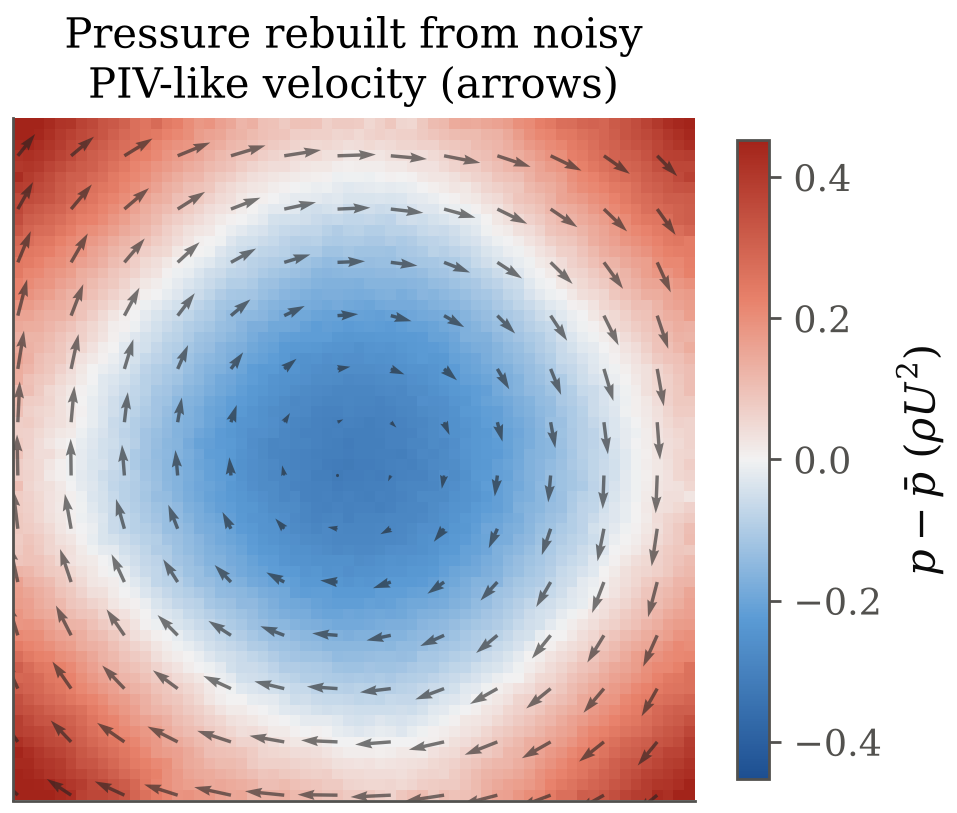
\includegraphics[width=0.48\linewidth]{img/f_hero.png}
\vfill
{\large Anany Bajpai (24B2135) \quad\textperiodcentered\quad Arnav Oza (24B2217)\par}
\vspace{0.2cm}
{\normalsize Instructor: Prof.\ Anjishnu Choudhury\par}
\vspace{0.2cm}
{\small\color{gray} Term project 6 \textperiodcentered{} Autumn 2026 \textperiodcentered{} Document version of 31 October 2026\par}
\end{titlepage}

\pagenumbering{roman}
\chapter*{How to read this document}
\addcontentsline{toc}{chapter}{How to read this document}
This document explains the whole project from the ground up. It assumes you know undergraduate fluid mechanics and basic numerical methods, and nothing about PIV or pressure reconstruction. It goes all the way down to individual stencils, matrix rows and the reasons behind every design decision, so you can defend any line of the code in a viva.

\begin{itemize}
  \item \textbf{Part I (Chapters 1--3)} builds the physics: what PIV measures, why pressure is not measured, and how the Navier--Stokes equations let us recover it.
  \item \textbf{Part II (Chapters 4--7)} builds the numerics: finite differences and how they amplify noise, the discrete Poisson problem and its singularity, the three integration algorithms, and the iterative solvers.
  \item \textbf{Part III (Chapters 8--9)} sets up the virtual experiment: exact flows, the synthetic PIV error model, metrics, and the code that runs it all.
  \item \textbf{Part IV (Chapters 10--11)} presents every result with the reason it comes out the way it does.
  \item \textbf{Part V (Chapters 12--14)} covers the OpenFOAM cylinder-wake simulation, the comparison with published studies, and the conclusions.
  \item \textbf{Appendices} collect viva questions with short answers, a file map, the run commands and the notation.
\end{itemize}

Three kinds of boxes recur:
\begin{keyidea}A result or principle worth remembering.\end{keyidea}
\begin{pitfall}Something that goes wrong if done naively, and what the project does instead.\end{pitfall}
\begin{viva}Questions an examiner is likely to ask, with short answers.\end{viva}

\textbf{Sources of the numbers.} Every analytic result comes from the project's own CSV files (\code{results/*.csv}, 10 noise seeds, deterministic). The cylinder-wake results in Chapter~12 come from the OpenFOAM runs (three meshes) and their post-processing scripts.

\tableofcontents

\clearpage
\pagenumbering{arabic}

% ================================================================== PART I
\part{Physics: what we want and why it is hard}

\chapter{The project in one picture}

\section{The question}
Pressure is one of the most useful quantities in fluid mechanics. It sets the lift and drag on a body, drives cavitation, and is the source of flow noise. Yet it is surprisingly hard to measure over a whole field:
\begin{itemize}
  \item \textbf{Pressure taps} and transducers give pressure only at a few points, and only on walls.
  \item \textbf{Probes} placed in the flow disturb the very flow they measure.
  \item \textbf{Pressure-sensitive paint} works only on surfaces.
\end{itemize}
\textbf{Particle Image Velocimetry (PIV)}, by contrast, measures the \emph{velocity} over a whole plane without touching the flow. The question of this project is:

\begin{keyidea}[The question]
Given only PIV-type velocity fields $\uu(x,y,t)$ (noisy, smoothed, on a finite grid), how accurately can we reconstruct the pressure field $p(x,y,t)$, which algorithm should we use, and what controls the error?
\end{keyidea}

\section{The answer in three steps}
The momentum equation links pressure to velocity. Rearranged, it gives the pressure \emph{gradient} as a function of velocity only:
\begin{equation}
\nabla p = \G \equiv -\rho\frac{D\uu}{Dt} + \mu\nabla^2\uu .
\end{equation}
So the recipe is:
\begin{enumerate}
  \item \textbf{Differentiate} the measured velocity (in space and time) to get $\G$.
  \item \textbf{Integrate} $\G$ to get $p$ (up to an additive constant).
  \item \textbf{Compare} with a known true pressure to measure the error.
\end{enumerate}
Step 1 is where the difficulty lives: differentiation amplifies measurement noise. Step 2 decides whether that noise is averaged out or accumulated. Step 3 needs data where the true pressure is known, which is why the project uses exact Navier--Stokes solutions and a CFD simulation as ``virtual experiments''.

\begin{figure}[H]
\centering
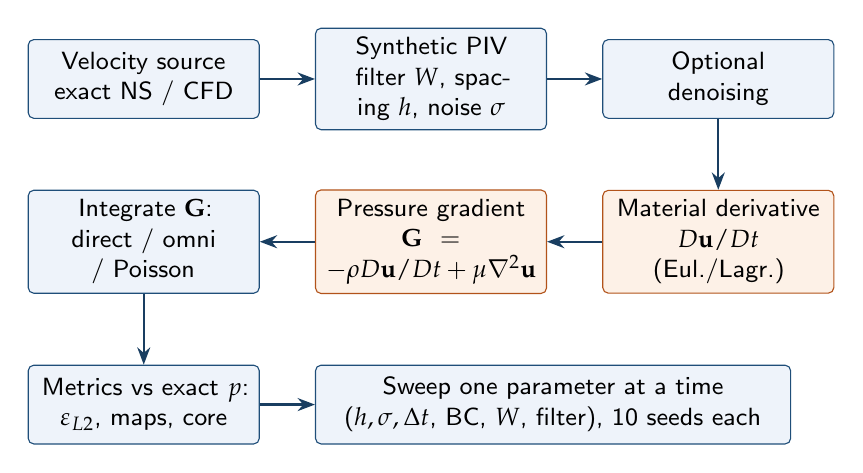
\begin{tikzpicture}[node distance=5mm and 7mm, every node/.style={font=\small\sffamily},
  box/.style={draw=accent,fill=boxbg,rounded corners=2pt,align=center,minimum height=10mm,text width=27mm},
  hot/.style={draw=warn,fill=warnbg,rounded corners=2pt,align=center,minimum height=10mm,text width=27mm},
  ar/.style={-{Stealth[length=2.2mm]},thick,color=accent!80!black}]
\node[box] (src) {Velocity source\\ exact NS / CFD};
\node[box,right=of src] (piv) {Synthetic PIV\\ filter $W$, spacing $h$, noise $\sigma$};
\node[box,right=of piv] (den) {Optional\\ denoising};
\node[hot,below=9mm of den] (dudt) {Material derivative\\ $D\uu/Dt$ (Eul./Lagr.)};
\node[hot,left=of dudt] (G) {Pressure gradient\\ $\G=-\rho D\uu/Dt+\mu\nabla^2\uu$};
\node[box,left=of G] (int) {Integrate $\G$:\\ direct / omni / Poisson};
\node[box,below=9mm of int] (met) {Metrics vs exact $p$:\\ $\eps_{L2}$, maps, core};
\node[box,right=of met,text width=58mm] (sw) {Sweep one parameter at a time\\ ($h,\sigma,\Delta t$, BC, $W$, filter), 10 seeds each};
\draw[ar] (src)--(piv); \draw[ar] (piv)--(den); \draw[ar] (den)--(dudt); \draw[ar] (dudt)--(G); \draw[ar] (G)--(int); \draw[ar] (int)--(met); \draw[ar] (met)--(sw);
\end{tikzpicture}
\caption{The whole project as one pipeline. Orange boxes are where noise is amplified (differentiation); the integration step decides whether it is averaged out.}
\end{figure}

\section{What was built}
\begin{itemize}
  \item A Python package (about 7\,500 lines, NumPy/SciPy/Matplotlib) with three reconstruction algorithms: \textbf{direct integration}, \textbf{omni-directional integration} and a \textbf{pressure-Poisson solver}, plus five Poisson solvers (sparse direct, Jacobi, Gauss--Seidel, SOR, conjugate gradient).
  \item A \textbf{synthetic PIV model} that degrades exact velocity fields like a real PIV system: window averaging, finite spacing, random noise.
  \item \textbf{Validation flows}: the Taylor--Green vortex (stationary and convected) and Kovasznay flow (Re 20 and 40), all exact solutions of Navier--Stokes.
  \item A \textbf{CFD case}: a 2-D laminar cylinder wake at Re = 100 in OpenFOAM, on three meshes, sampled in a PIV-like window.
  \item \textbf{Studies} of grid spacing, noise, time step, boundary conditions, integration method, window size and denoising; a convergence and error-analysis study (norms, residuals, solver stability, scheme order).
  \item \textbf{87 unit tests}, all passing, which check every stencil, solver and parser against exact answers.
\end{itemize}

% ------------------------------------------------------------------
\chapter{Particle Image Velocimetry}

\section{How PIV works}
\begin{figure}[H]\centering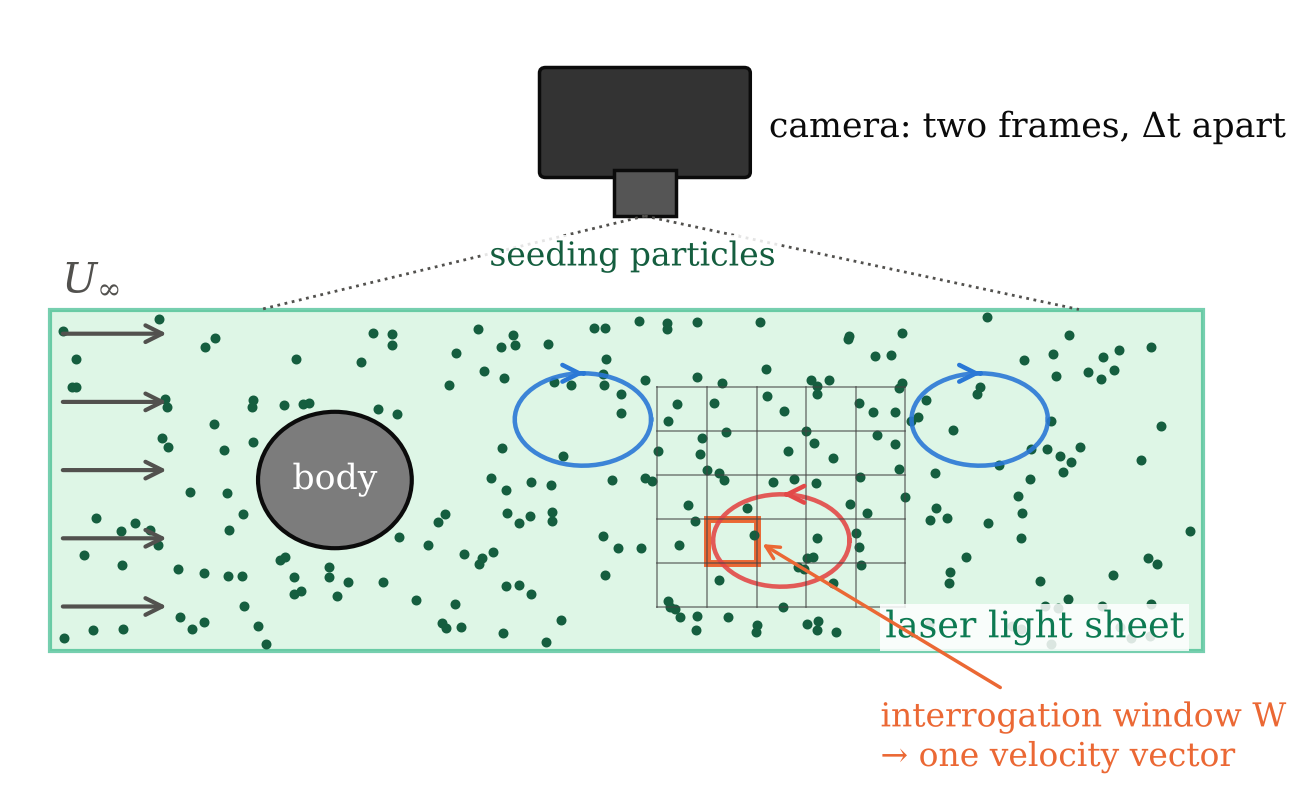
\includegraphics[width=0.62\linewidth]{img/f_piv_schematic.png}
\caption{Planar PIV. A laser sheet lights seeding particles; a camera records two frames $\Delta t$ apart; each interrogation window yields one velocity vector.}\end{figure}
\begin{enumerate}
  \item The flow is seeded with small tracer particles that follow it faithfully.
  \item A thin laser sheet illuminates a plane of the flow.
  \item A camera takes two images a short time $\Delta t$ apart.
  \item Each image is cut into small \textbf{interrogation windows} of size $W$. Cross-correlating a window in frame 1 with the same window in frame 2 gives the most likely particle displacement $\Delta\mathbf{x}$ in that window.
  \item The velocity of the window is $\uu = \Delta\mathbf{x}/\Delta t$. Repeating over all windows gives a vector field on a grid of spacing $h$ (often $h=W/2$ with 50\,\% overlap).
  \item \textbf{Time-resolved PIV} repeats this at high frame rate, giving a sequence of fields $\uu^{n-1},\uu^n,\uu^{n+1},\dots$ This is what the time derivative in $D\uu/Dt$ needs.
\end{enumerate}

\section{What PIV gets wrong}
Every pressure error in this project traces back to three properties of PIV data. The synthetic model in Chapter~8 reproduces exactly these three.
\begin{description}[style=nextline]
  \item[1. Spatial averaging (window $W$)] A vector is an average over the window, so it acts like a low-pass filter. Peaks are flattened and sharp gradients are smeared. For a box average of width $W$ the transfer function is $\sin(kW/2)/(kW/2)\approx 1-(kW)^2/24$, i.e.\ the measured velocity is biased by about $-(W^2/24)\nabla^2\uu$.
  \item[2. Finite spacing ($h$)] Derivatives must be estimated by finite differences on a grid of spacing $h$; their truncation error falls as $h^2$ but noise amplification grows as $1/h$ or $1/h^2$.
  \item[3. Random error ($\sigma$)] Correlation peaks are located with an uncertainty of order 0.1 pixel, giving a random velocity error typically 0.5--2\,\% of the flow speed. We model it as independent Gaussian noise of standard deviation $\sigma U$.
\end{description}
Real PIV adds further errors: out-of-plane motion (planar PIV misses $w$ and $\partial/\partial z$), particle lag, peak locking, and outliers. These are discussed as limitations in Chapter~14.

% ------------------------------------------------------------------
\chapter{From velocity to pressure: the governing equations}

\section{Pressure gradient from Navier--Stokes}
For an incompressible Newtonian fluid with constant density $\rho$ and viscosity $\mu$:
\begin{equation}
\nabla\cdot\uu = 0, \qquad
\rho\left(\frac{\partial\uu}{\partial t}+(\uu\cdot\nabla)\uu\right) = -\nabla p + \mu\nabla^2\uu .
\label{eq:ns}
\end{equation}
Solve the momentum equation for $\nabla p$:
\begin{equation}
\boxed{\;\nabla p = \G \equiv -\rho\frac{D\uu}{Dt}+\mu\nabla^2\uu, \qquad \frac{D\uu}{Dt}=\frac{\partial\uu}{\partial t}+(\uu\cdot\nabla)\uu\;}
\label{eq:G}
\end{equation}
In two dimensions, component by component (this is literally what \code{core/material\_derivative.py} computes):
\begin{align}
G_x &= -\rho\,(u_t + u\,u_x + v\,u_y) + \mu\,(u_{xx}+u_{yy}),\\
G_y &= -\rho\,(v_t + u\,v_x + v\,v_y) + \mu\,(v_{xx}+v_{yy}).
\end{align}
\begin{itemize}
  \item $D\uu/Dt$ is the \textbf{material (particle) acceleration}. It dominates at moderate and high Reynolds number.
  \item $\mu\nabla^2\uu$ is the \textbf{viscous term}. It matters at low Reynolds number: for Kovasznay flow at Re = 20 or 40, dropping it leaves an $O(1)$ error that never converges (a unit test checks this).
  \item In the non-dimensional CFD setup $\rho=1$, so $p$ is the \emph{kinematic} pressure $p/\rho$, exactly what OpenFOAM's incompressible solvers use.
\end{itemize}

\begin{keyidea}[Why this is an inverse problem]
Every term of $\G$ is a \emph{derivative} of measured data. So pressure from PIV is the inverse of differentiation: the data are differentiated (which amplifies noise) and then integrated (which can smooth it again). Everything else in the project is about doing these two operations well.
\end{keyidea}

\section{The material derivative: two ways to estimate it}

\subsection{Eulerian (fixed point)}
At a fixed grid node, with three snapshots $n-1,n,n+1$:
\begin{equation}
\left(\frac{D\uu}{Dt}\right)_E \approx \frac{\uu^{n+1}-\uu^{n-1}}{2\Delta t} + (\uu^n\cdot\nabla)\uu^n .
\end{equation}
The time difference has truncation error $-(\Delta t^2/6)\,\partial^3\uu/\partial t^3$: second order.

\subsection{Lagrangian (follow the particle)}
Instead of sitting at a point, follow a fluid particle along a straight path through the node with the local velocity $\mathbf{a}=\uu(\mathbf{x},t^n)$:
\begin{equation}
\left(\frac{D\uu}{Dt}\right)_L \approx \frac{\uu(\mathbf{x}+\mathbf{a}\Delta t,\,t^{n+1})-\uu(\mathbf{x}-\mathbf{a}\Delta t,\,t^{n-1})}{2\Delta t}.
\end{equation}
The velocities at the off-grid points come from cubic interpolation.

\textbf{Accuracy.} Let $L=\partial/\partial t+\mathbf{a}\cdot\nabla$ with $\mathbf{a}$ frozen. A shift in space and time is the exponential of $L$: $\uu(\mathbf{x}\pm\mathbf{a}\Delta t,t\pm\Delta t)=e^{\pm\Delta t L}\uu$. Then
\begin{equation}
\left(\frac{D\uu}{Dt}\right)_L=\frac{\sinh(\Delta t L)}{\Delta t}\uu = L\uu+\frac{\Delta t^2}{6}L^3\uu+O(\Delta t^4),
\end{equation}
and $L\uu$ is exactly $D\uu/Dt$. So the Lagrangian scheme is also second order in $\Delta t$; what differs is the \emph{size} of the error constant.

\begin{keyidea}[When Lagrangian wins]
Take a flow pattern $\mathbf{w}$ carried along at speed $\mathbf{c}$: $\uu(\mathbf{x},t)=\mathbf{c}+\mathbf{w}(\mathbf{x}-\mathbf{c}t)$.
\begin{itemize}
\item Eulerian error $\propto \partial^3\uu/\partial t^3 = -(\mathbf{c}\cdot\nabla)^3\mathbf{w}$, which scales like $c^3$.
\item Lagrangian error $\propto L^3\uu=(\mathbf{w}\cdot\nabla)^3\mathbf{w}$, which scales like $w^3$.
\end{itemize}
In a wake the vortices are \emph{carried} faster ($c\approx U$) than they \emph{spin} ($w<c$), so the Lagrangian estimate is more accurate at large $\Delta t$. For a stationary vortex ($c=0$) the Eulerian time error is almost zero and the Lagrangian one is larger. The project verifies both cases (Section~10.5).
\end{keyidea}

\begin{pitfall}[SciPy cubic interpolation]
Since SciPy 1.13, \code{RegularGridInterpolator(method="cubic")} computes spline coefficients with an iterative solver (atol $10^{-6}$). The interpolation error then stalls near $10^{-5}$ whatever the grid, and the Lagrangian error \emph{grows} under refinement. The code requests the direct solver (\code{solver=spsolve}), which restores fourth-order interpolation. Where the tracked point leaves the window, the code falls back to the Eulerian value and reports the fraction of such nodes.
\end{pitfall}

\section{The pressure-Poisson equation}
Taking the divergence of $\nabla p=\G$ gives an elliptic problem with Neumann boundary conditions:
\begin{equation}
\boxed{\;\nabla^2 p = \nabla\cdot\G \;\text{ in }\Omega, \qquad \frac{\partial p}{\partial n}=\n\cdot\G \;\text{ on }\partial\Omega\;}
\label{eq:poisson}
\end{equation}

\subsection{Compatibility}
Integrate the Poisson equation over the domain and use Gauss's theorem: $\iint_\Omega\nabla^2p\,dA=\oint_{\partial\Omega}\partial p/\partial n\,ds$. A solution exists only if
\begin{equation}
R \equiv \iint_\Omega\nabla\cdot\G\,dA-\oint_{\partial\Omega}\n\cdot\G\,ds = 0 .
\end{equation}
For an exact gradient field $R=0$ automatically. For discretised or noisy $\G$ it is not, and the code reports $R$ (\code{compatibility\_residual}). Even when it holds, the solution is unique only up to a constant: adding any constant to $p$ changes nothing.

\subsection{Poisson as a least-squares projection}
Measured $\G$ is not exactly a gradient: it has a non-zero curl, which can only be error (the curl of a true gradient is zero). What is the ``best'' pressure? Minimise the mismatch
\begin{equation}
J[p]=\iint_\Omega|\nabla p-\G|^2\,dA .
\end{equation}
The calculus of variations gives the Euler--Lagrange equation $\nabla^2p=\nabla\cdot\G$ in $\Omega$ and the natural boundary condition $\partial p/\partial n=\n\cdot\G$ on $\partial\Omega$: exactly Eq.~\eqref{eq:poisson}.

\begin{keyidea}[Why Poisson is robust]
The Poisson problem \emph{projects} the measured $\G$ onto the space of gradient fields. It keeps the curl-free part and discards the curl, which is pure error. That is why Poisson reconstruction is path-independent and filters noise, and why the source term and the boundary data must come from the \emph{same} $\G$ (Section~10.3 shows what happens otherwise).
\end{keyidea}

\subsection{An alternative source term (2-D incompressible identity)}
Take the divergence of $\G$ term by term. $\nabla\cdot(\partial\uu/\partial t)=\partial(\nabla\cdot\uu)/\partial t=0$ and $\nabla\cdot\nabla^2\uu=\nabla^2(\nabla\cdot\uu)=0$. Only the convective term survives:
\begin{equation}
\nabla\cdot((\uu\cdot\nabla)\uu)=(\partial_iu_j)(\partial_ju_i)+u_j\partial_j(\partial_iu_i)=u_x^2+2u_yv_x+v_y^2,
\end{equation}
so
\begin{equation}
\nabla^2p=-\rho\left(u_x^2+2u_yv_x+v_y^2\right).
\end{equation}
This form needs no time derivative and no viscous term, which looks attractive. But it assumes $\nabla\cdot\uu=0$ exactly (noisy PIV data are not solenoidal), it multiplies noisy derivatives together (a bias of order $\sigma^2/h^2$), and its boundary data still come from $\G$. Section~10.3 shows that it is 5--8$\times$ worse on noisy data.

\textit{Check on Taylor--Green:} $u_x=-\sin x\sin y\,F$, $v_y=\sin x\sin y\,F$, $u_y=\cos x\cos y\,F$, $v_x=-\cos x\cos y\,F$, so $-\rho(2\sin^2x\sin^2y-2\cos^2x\cos^2y)F^2=\rho(\cos2x+\cos2y)F^2=\nabla^2p$. \checkmark

\section{Bernoulli boundary values}
For \textbf{steady, irrotational} flow, $p+\tfrac12\rho|\uu|^2$ is constant along the whole field, so a free-stream edge could be given the Dirichlet value
\begin{equation}
p=p_\infty+\tfrac12\rho\,(U_\infty^2-|\uu|^2).
\end{equation}
For unsteady irrotational flow the correct form is $p+\rho\,\partial\phi/\partial t+\tfrac12\rho|\uu|^2=\text{const}$, and in rotational flow there is no such relation at all. Both validation flows carry vorticity everywhere, so Bernoulli edges \emph{must} fail there; the project tests this deliberately (Section~10.4).

\begin{viva}
\begin{enumerate}[leftmargin=*]
\item \emph{Why can't PIV measure pressure directly?} It measures particle displacement, i.e.\ velocity. Pressure enters only through the momentum equation.
\item \emph{Why is the result only defined up to a constant?} Only $\nabla p$ is known; a constant has zero gradient. We compare $p-\bar p$ with $p_{ref}-\bar p_{ref}$.
\item \emph{When can you neglect the viscous term?} At high Reynolds number away from walls; never in Kovasznay flow at Re 20--40.
\item \emph{What does the compatibility condition mean physically?} The total ``source'' inside must equal the net flux through the boundary; a non-gradient $\G$ violates it.
\item \emph{Why does Poisson filter noise?} It is the least-squares fit of a gradient field to $\G$; the curl part (pure error) is discarded.
\end{enumerate}
\end{viva}

% ================================================================== PART II
\part{Numerics: turning the equations into code}

\chapter{Finite differences and noise amplification}

\section{Stencils used everywhere}
All spatial derivatives use second-order finite differences on the uniform PIV grid (spacing $h$), including at the edges.

\begin{table}[H]\centering\small
\begin{tabular}{@{}llll@{}}\toprule
Quantity & Where & Stencil & Truncation error\\\midrule
$f'$ & interior & $(f_{i+1}-f_{i-1})/2h$ & $-\tfrac{h^2}{6}f'''$\\
$f'$ & left edge & $(-3f_0+4f_1-f_2)/2h$ & $+\tfrac{h^2}{3}f'''$\\
$f''$ & interior & $(f_{i+1}-2f_i+f_{i-1})/h^2$ & $-\tfrac{h^2}{12}f''''$\\
$f''$ & left edge & $(2f_0-5f_1+4f_2-f_3)/h^2$ & $+\tfrac{11h^2}{12}f''''$\\
$\partial_t f$ & middle snapshot & $(f^{n+1}-f^{n-1})/2\Delta t$ & $-\tfrac{\Delta t^2}{6}f_{ttt}$\\\bottomrule
\end{tabular}
\caption{The finite-difference stencils (\code{core/derivatives.py}). The right edge mirrors the left.}
\end{table}

\textbf{Deriving the one-sided first derivative.} Expand about $x_0$:
$f_1=f_0+hf'+\tfrac{h^2}{2}f''+\tfrac{h^3}{6}f'''$ and $f_2=f_0+2hf'+2h^2f''+\tfrac{4h^3}{3}f'''$.
Look for $(af_0+bf_1+cf_2)/h$ whose $f_0$ and $f''$ coefficients vanish and whose $f'$ coefficient is 1:
\[
a+b+c=0,\qquad b+2c=1,\qquad \tfrac b2+2c=0 \;\Rightarrow\; a=-\tfrac32,\; b=2,\; c=-\tfrac12 .
\]
The same procedure with four points (cancel $f_0,f',f'''$, keep $f''$) gives $(2,-5,4,-1)/h^2$.

\begin{pitfall}[Boundary stencils must be second order too]
The Neumann data $\n\cdot\G$ and the source term on the boundary rows are computed with these edge stencils. A first-order stencil there would pull the \emph{global} order of the whole reconstruction down to 1. (Chapter~11 shows this deliberately with \code{order=1}.)
\end{pitfall}

\section{How differentiation amplifies noise}
Suppose every velocity sample carries independent noise of standard deviation $s=\sigma U$. Linear combinations of independent errors add in variance:
\begin{align}
\text{time difference: }&\operatorname{std}\!\left[\frac{\epsilon^{n+1}-\epsilon^{n-1}}{2\Delta t}\right]=\frac{\sqrt2\,s}{2\Delta t}=\frac{s}{\sqrt2\,\Delta t},\\
\text{first derivative: }&\frac{s}{\sqrt2\,h},\\
\text{5-point Laplacian: }&\frac{\sqrt{1^2+1^2+1^2+1^2+4^2}\;s}{h^2}=\frac{\sqrt{20}\,s}{h^2}.
\end{align}
Putting these into $\G$:
\begin{equation}
\operatorname{noise}(\G)\sim \underbrace{\rho\frac{s}{\sqrt2\Delta t}}_{\partial\uu/\partial t}+\underbrace{\rho U\frac{s}{\sqrt2 h}}_{\text{convective}}+\underbrace{\mu\frac{\sqrt{20}\,s}{h^2}}_{\text{viscous}} .
\label{eq:noiseG}
\end{equation}

\begin{keyidea}[The central tension of the whole project]
Truncation error falls as $h^2$ and $\Delta t^2$, but noise amplification grows as $1/h$, $1/h^2$ and $1/\Delta t$. Refining the measurement therefore helps only up to a point. Below an optimum spacing the error \emph{rises} again. Minimising $E(h)\approx Ch^2+K\sigma/h^q$ gives $h_{opt}\propto\sigma^{1/(2+q)}$: noisier data need a coarser grid.
\end{keyidea}

\begin{figure}[H]\centering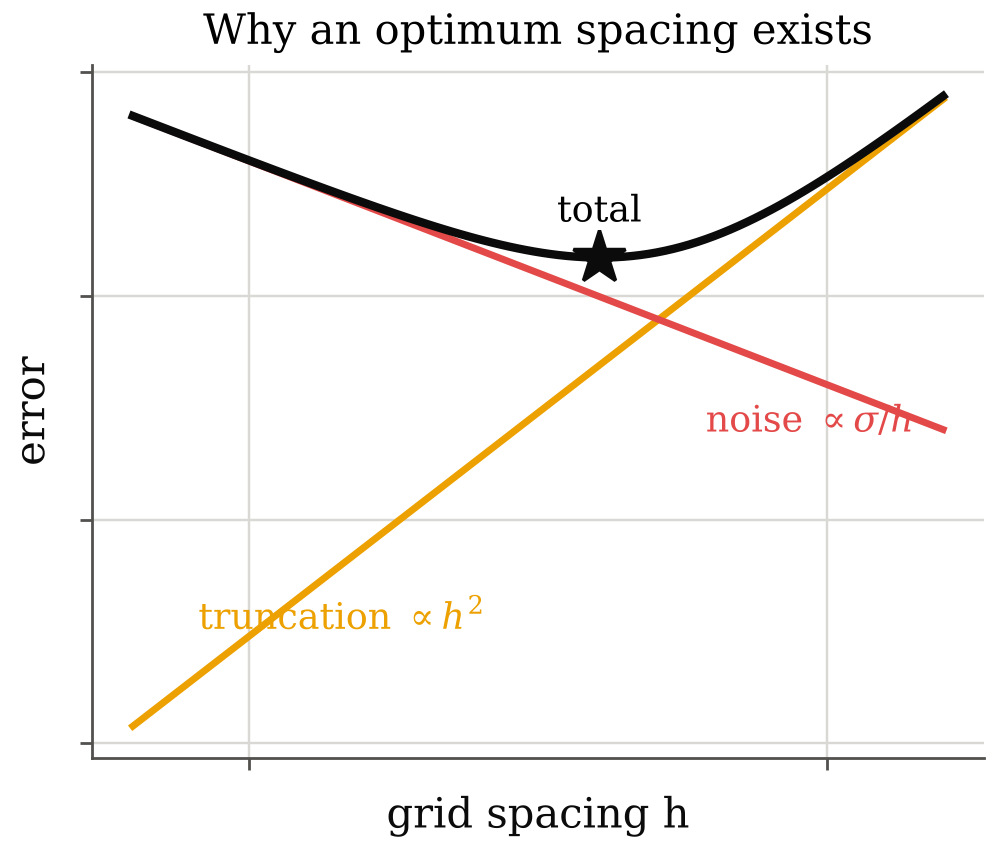
\includegraphics[width=0.45\linewidth]{img/f_tradeoff.png}
\caption{Error budget (schematic): truncation error falls with $h$, noise amplification rises, and the total has a minimum.}\end{figure}

% ------------------------------------------------------------------
\chapter{The discrete pressure-Poisson problem}

\section{The 5-point Laplacian}
Unknowns $p_{i,j}$ sit at the PIV nodes, numbered $k=j\,n_x+i$. In the interior,
\begin{equation}
\frac{p_{i+1,j}-2p_{i,j}+p_{i-1,j}}{\Delta x^2}+\frac{p_{i,j+1}-2p_{i,j}+p_{i,j-1}}{\Delta y^2}=f_{i,j}=(\nabla\cdot\G)_{i,j},
\end{equation}
with truncation error $-\tfrac{\Delta x^2}{12}p_{xxxx}-\tfrac{\Delta y^2}{12}p_{yyyy}$. The matrix is assembled with Kronecker products, $A=I_y\otimes D_{xx}+D_{yy}\otimes I_x$, and stored as a sparse CSR matrix.

\section{Neumann boundaries by ghost-point elimination}
At the left edge ($i=0$) invent a ghost node $i=-1$ outside the domain. Discretise the Neumann condition $\partial p/\partial x=G_x$ centrally:
\begin{equation}
\frac{p_1-p_{-1}}{2\Delta x}=G_{x,0}\quad\Rightarrow\quad p_{-1}=p_1-2\Delta x\,G_{x,0}.
\end{equation}
Substitute into the Laplacian row at $i=0$ and move the known part to the right-hand side:
\begin{equation}
\frac{2p_1-2p_0}{\Delta x^2}+[\,y\text{-part}\,]=f_0+\frac{2G_{x,0}}{\Delta x}.
\end{equation}
The other edges follow the same pattern: right edge $b\mathrel{-}=2G_x/\Delta x$, bottom $b\mathrel{+}=2G_y/\Delta y$, top $b\mathrel{-}=2G_y/\Delta y$. In 1-D the operator becomes the matrix with rows $[-2,\,2]$, $[1,-2,1],\dots,[2,-2]$, all divided by $h^2$.

\textbf{Corners} have two ghost neighbours, one in $x$ and one in $y$. Each is eliminated with \emph{its own} condition ($\partial p/\partial x=G_x$ and $\partial p/\partial y=G_y$), so both are used exactly. Averaging the two conditions (as the original project specification suggested) would throw information away.

\textbf{Order of accuracy.} The boundary rows have local truncation error $O(h)$, since $(2p_1-2p_0)/h^2-2g/h=p''+\tfrac h3p'''+\dots$ But the global error is still $O(h^2)$:
\begin{itemize}
\item the $O(h)$ error lives on a strip of width $O(h)$ only;
\item multiplying edge rows by $\tfrac12$ and corner rows by $\tfrac14$ turns the scheme into a vertex-centred finite-volume scheme on half and quarter cells, whose flux errors are $O(h^2)$.
\end{itemize}
The tests confirm global slopes of 1.8--2.2.

\textbf{Symmetric form.} With trapezoidal weights $w$ (1 inside, $\tfrac12$ on edges, $\tfrac14$ at corners) and $W=\operatorname{diag}(w)$, the matrix $WA$ is symmetric and $S=-WA$ is symmetric positive semi-definite. Conjugate gradients needs exactly this.

\section{The all-Neumann system is singular}
$A\mathbf{1}=0$: adding a constant to $p$ changes nothing, so $A$ has a one-dimensional null space and the pressure is fixed only up to a constant. The left null vector is $w$ ($w^TA=0$), so $Ap=b$ is solvable only if $w^Tb=0$, and
\begin{equation}
\Delta x\,\Delta y\,w^Tb=\text{trapezoidal}\iint f\,dA-\text{trapezoidal}\oint\n\cdot\G\,ds ,
\end{equation}
the \emph{discrete compatibility residual}. Two fixes are implemented:

\begin{description}[style=nextline]
\item[\code{pin="node"}: replace one row by $p_k=0$]
The system becomes solvable, but the discarded row was the only place the incompatibility $R$ could go. $R$ then acts as a point source at the pinned node, producing a logarithmic disturbance $\sim(R/2\pi)\ln r$ around it. Errors are larger: on clean Taylor--Green $5.8\times10^{-3}$ vs $7.2\times10^{-4}$.
\item[\code{pin="mean"} (default): zero-mean augmented system]
\begin{equation}
\begin{bmatrix}A&\mathbf 1\\\mathbf 1^T&0\end{bmatrix}\begin{bmatrix}p\\\lambda\end{bmatrix}=\begin{bmatrix}b\\0\end{bmatrix}
\quad\Longleftrightarrow\quad Ap+\lambda\mathbf 1=b,\;\;\textstyle\sum p=0.
\end{equation}
Multiplying the first row by $w^T$ gives $\lambda=w^Tb/w^T\mathbf 1$: a \emph{uniform} source correction spreads the incompatibility evenly instead of dumping it at one node. The bordered matrix is non-singular because $\mathbf1$ is not in the range of $A$ ($w^T\mathbf 1\neq0$).
\end{description}

\textbf{Dirichlet edges} (known pressure, from taps or Bernoulli) replace those rows by $p_k=$ value. Such an edge fixes the constant, so no pin is needed.

\begin{viva}
\begin{enumerate}[leftmargin=*]
\item \emph{Why is the all-Neumann matrix singular?} $A\mathbf 1=0$; fix it by pinning a node or adding a zero-mean constraint.
\item \emph{Why is pin-mean better than pin-node?} Pin-node dumps the incompatibility $R$ at one point (a point source); pin-mean spreads it uniformly.
\item \emph{What does $\lambda$ represent?} The uniform source correction that makes the data compatible.
\item \emph{Why is the global error second order if boundary rows are first order?} The $O(h)$ error acts only on an $O(h)$ strip; equivalently the scaled scheme is a second-order finite-volume scheme.
\end{enumerate}
\end{viva}

% ------------------------------------------------------------------
\chapter{Direct and omni-directional integration}

\begin{figure}[H]\centering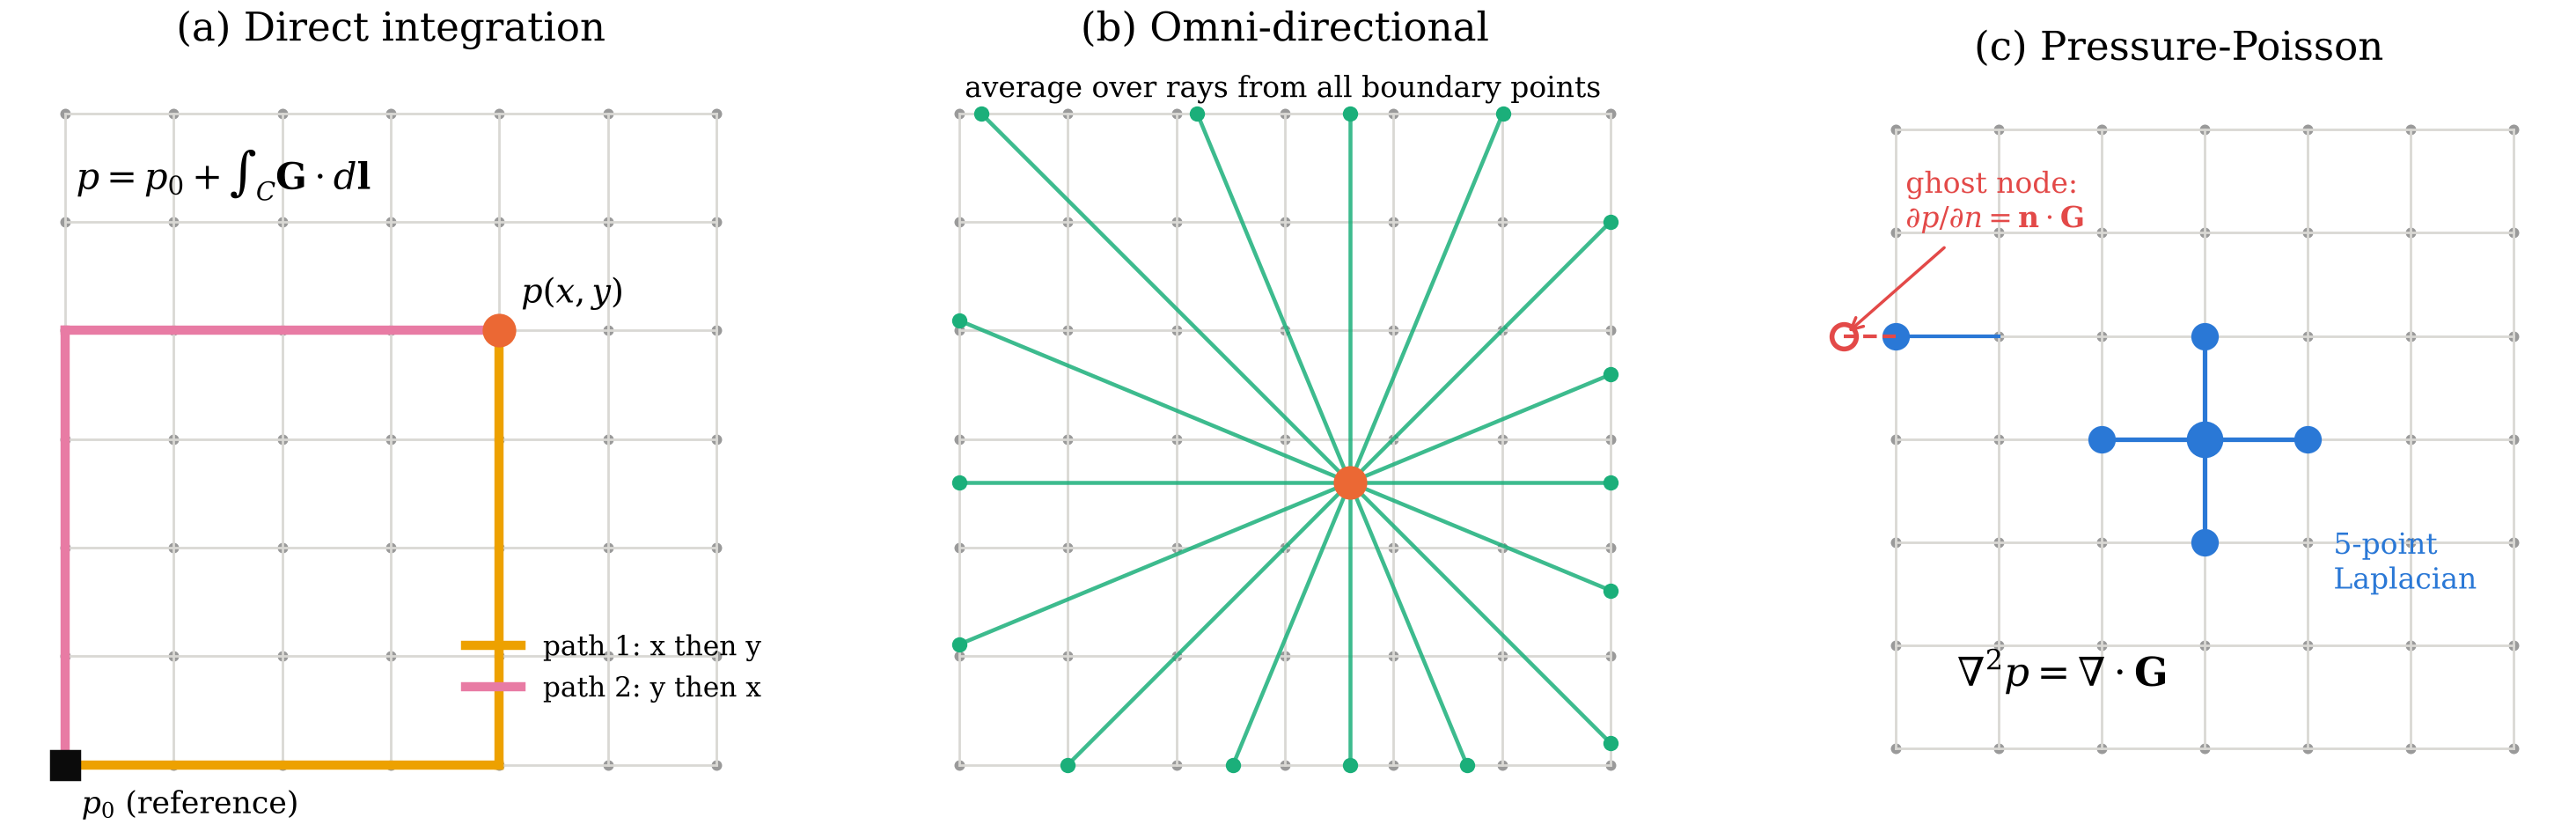
\includegraphics[width=\linewidth]{img/f_methods.png}
\caption{The three algorithms on the PIV grid: (a) direct integration along two paths, (b) omni-directional rays from all directions, (c) the Poisson stencil with a ghost node.}\end{figure}

\section{Direct spatial integration}
The simplest idea: integrate the gradient along a path from a reference point,
\begin{equation}
p(B)-p(A)=\int_A^B\G\cdot d\mathbf l,
\end{equation}
using the cumulative trapezoidal rule (second order).
\begin{itemize}
\item \textbf{Path 1:} along the first row in $x$, then up each column in $y$.
\item \textbf{Path 2:} along the first column in $y$, then along each row in $x$.
\item The code reports both and their average.
\end{itemize}
For an exact gradient both paths agree (Stokes: $\oint\G\cdot d\mathbf l=\iint\operatorname{curl}\G\,dA=0$). Measured $\G$ has a curl, so they differ; the difference measures path dependence.

\begin{keyidea}[Why direct integration is so noise-sensitive]
Along a path of $N=L/h$ steps the trapezoidal sum adds $N$ independent errors of size $h\,\sigma_G$. They add like a random walk: error $\propto h\,\sigma_G\sqrt{N}=\sigma_G\sqrt{hL}$. With $\sigma_G\sim s/h$ from the derivatives this is $\propto s\sqrt{L/h}$, which \emph{grows} as the grid is refined, and faster still where the viscous noise $\sim s/h^2$ matters. Every error made early on the path is carried to every later point.
\end{keyidea}

\section{Omni-directional integration}
Liu \& Katz (2006) proposed averaging line integrals over many paths from all directions, so that path errors cancel. The project implements a \emph{rotating-ray} variant (\code{core/omni\_integration.py}):
\begin{enumerate}
\item Directions $\theta_k=2\pi k/N$, $k=0,\dots,N-1$, with $N=32$.
\item From every node $P$, trace a straight ray backwards to the boundary point $E_k(P)$ and integrate $\G\cdot\mathbf e_k$ from $E_k$ to $P$ (trapezoidal rule, step $h$, bilinear interpolation of $\G$).
\item \textbf{Boundary stage.} Boundary values depend on each other through the rays: $p_i=\operatorname{mean}_k\big[\sum_mA_{im}p_m+I_i\big]$, i.e.\ a linear system $(I-A)p_b=c$. Its null space is the constants and it is not exactly compatible (curl $\G\neq0$), so it is solved with the same zero-mean augmented system as above.
\item \textbf{Interior stage.} $p(P)=\operatorname{mean}_k\big[p_b(E_k)+\int\G\cdot\mathbf e_k\,ds\big]$.
\end{enumerate}
The original paper uses a virtual boundary with parallel rays and iterates the boundary values. This version keeps the principle (many directions, boundary values consistent with the rays) but starts the rays at each node.

\textbf{Cost.} $O(N\times\text{nodes}\times\text{ray length})$: about 0.4\,s at $64^2$ against 15\,ms for Poisson. That is why the noisy grid study runs omni only up to $64^2$.

% ------------------------------------------------------------------
\chapter{Iterative solvers, norms and convergence}
The default Poisson solver is a sparse direct factorisation (\code{scipy.sparse.linalg.spsolve}). The course (Lecture 11) asks how iterative solvers behave, how to judge convergence, and how to measure residuals. The project implements all of this on the same matrix.

\section{Norms of a residual}
For a residual vector $r$ with $n$ entries:
\begin{table}[H]\centering\small
\begin{tabular}{@{}lll@{}}\toprule
Norm & Formula & Meaning\\\midrule
$L_1$ & $\sum|r_i|$ & total absolute imbalance\\
$L_2$ & $\sqrt{\sum r_i^2}$ & Euclidean length; large entries dominate\\
$L_\infty$ & $\max|r_i|$ & worst cell only\\
$L_{1n}$ & $\tfrac1n\sum|r_i|$ & mean imbalance per cell\\
$L_{2n}$ & $\sqrt{\tfrac1n\sum r_i^2}$ & RMS imbalance per cell\\
scaled & $L_{2n}(r)/S$ & relative imbalance ($S=L_{2n}(b)$)\\\bottomrule
\end{tabular}\end{table}
For a residual of constant size $c$ on $n$ cells, $L_1=nc$ and $L_2=\sqrt n\,c$ grow with the grid while $L_{1n}=L_{2n}=c$ do not. A fixed tolerance on an unnormalised norm is therefore harder to meet the finer the grid; the project measures exponents 0.99 ($L_1$) and 0.50 ($L_2$) vs about 0 for the normalised norms. Always $L_{1n}\le L_{2n}\le L_\infty$.

\emph{Lecture example} (a unit test): $r=(0.0001,0.0004,0.0006,0.002)$ gives $L_1=0.0031$, $L_2=0.00213$, $L_{2n}=0.00106$.

With $p^0=0$ the first residual is $b$, so the scaled residual starts at exactly 1, and ``tol $=10^{-8}$'' means ``reduce the imbalance by $10^8$''.

\section{Jacobi is pseudo-time marching}
Jacobi updates $p^{k+1}=p^k+\omega D^{-1}(b-Ap^k)$ with $D=\operatorname{diag}A$. For $\Delta x=\Delta y=h$ every diagonal entry is $-4/h^2$, so
\begin{equation}
p^{k+1}=p^k+\underbrace{\omega\frac{h^2}{4}}_{\Delta\tau}\left(\nabla_h^2p^k-f\right),
\end{equation}
which is explicit Euler time-stepping of the pseudo-transient equation $\partial p/\partial\tau=\nabla^2p-f$ toward its steady state $\nabla^2p=f$.

\textbf{Stability.} Each eigenmode is multiplied by $1+\Delta\tau\lambda$, with $\lambda\in[-8/h^2,0]$ for the 5-point Laplacian. Stability needs $|1-8\Delta\tau/h^2|\le1$, i.e.\ $\Delta\tau\le h^2/4$, which is exactly classic Jacobi ($\omega=1$).

\begin{pitfall}[Classic Jacobi stalls on the all-Neumann problem]
At $\Delta\tau=h^2/4$ the checkerboard mode $(-1)^{i+j}$ (eigenvalue $-8/h^2$) is multiplied by $-1$ every step: it flips sign and never decays. With all-Neumann walls the checkerboard is an \emph{exact} eigenvector, so the residual levels off at a floor ($4.2\times10^{-8}$ at $64^2$, above tol $10^{-8}$). The project uses $\omega=0.95$ by default (amplification $-0.9$), which converges at a 5\,\% cost.
\end{pitfall}

\textbf{Convergence rate.} The smoothest mode decays by $1-\omega\mu_{min}$ per step with $\mu_{min}\approx(\pi h/L)^2/4$. Reducing the residual by a factor $F$ takes about $\ln F/\mu_{min}\propto(L/h)^2\propto N$ iterations: Jacobi's count grows linearly with the number of unknowns.

\section{Gauss--Seidel and SOR}
Gauss--Seidel uses the newest values as soon as they are available; SOR over-relaxes the update by $\omega$. The code uses \textbf{red-black ordering} (all nodes with $i+j$ even, then all odd), which vectorises each half-sweep and is ``consistently ordered'', so Young's theory applies:
\begin{itemize}
\item $\rho_{GS}=\rho_J^2$: Gauss--Seidel needs half the Jacobi iterations (measured 12\,328 vs 25\,366 at $64^2$).
\item SOR is optimal at $\omega_{opt}=2/\big(1+\sqrt{1-\rho_J^2}\big)$ with $\rho_{SOR}=\omega_{opt}-1$; the iteration count then scales like $\sqrt N$ instead of $N$.
\end{itemize}
\textbf{Neumann vs Dirichlet.} The textbook formula $\omega_{opt}=2/(1+\sin(\pi h/L))$ assumes Dirichlet walls ($\rho_J=\cos\pi h/L$). With all-Neumann walls the slowest non-constant mode varies in one direction only, $\rho_J=\cos^2(\pi h/2L)$, so the optimum is larger: 1.932 instead of 1.905 at $64^2$. The measured best $\omega$ is 1.9319 (314 iterations); the Dirichlet formula needs 628.

\textbf{Kahan's theorem:} $\rho_{SOR}\ge|\omega-1|$, so SOR cannot converge for $\omega\ge2$. The project shows $\omega=2$ (no decay) and $\omega=2.1$ (divergence to $10^{10}$ in 145 iterations).

\section{Conjugate gradient}
CG minimises the error in the energy norm over a growing Krylov space. It needs a symmetric positive (semi-)definite matrix, so it runs on $S=-WA$ (same equations, rows scaled by their trapezoidal weights) with a Jacobi preconditioner. Its iteration count scales like $\sqrt{\kappa(S)}\sim L/h\propto\sqrt N$. For the singular zero-mean problem it converges from $p^0=0$ because the right-hand side is made compatible.

\section{Residual vs change: when is a solution converged?}
For Jacobi, $p^{k+1}-p^k=\omega D^{-1}r^k$, so $\|p^{k+1}-p^k\|=\Delta\tau\|r^k\|$ with $\Delta\tau\approx3\times10^{-4}$ at $64^2$: the change is $10^3$--$10^4$ times smaller than the residual. Worse, the true error is $\|p^k-p^*\|\approx\|p^{k+1}-p^k\|/(1-\rho)$, and $1/(1-\rho)$ is huge when convergence is slow.

\begin{keyidea}[Do not stop on a small change alone]
A small change per iteration does \emph{not} mean convergence when convergence is slow. In the project, the change first drops below $10^{-6}$ at iteration 6\,697 while the scaled residual is still $6.1\times10^{-4}$ and the true error $1.7\times10^{-3}$. The solvers therefore stop on the scaled residual. The same logic applies to declaring a CFD run ``steady''.
\end{keyidea}

\begin{viva}
\begin{enumerate}[leftmargin=*]
\item \emph{Show that Jacobi is explicit pseudo-time marching.} $D^{-1}=-h^2/4$, so $p^{k+1}=p^k+\Delta\tau(\nabla^2_hp^k-f)$ with $\Delta\tau=\omega h^2/4$.
\item \emph{Why does classic Jacobi stall here but not with Dirichlet walls?} The Neumann checkerboard mode has amplification exactly $-1$; Dirichlet walls shift the extreme eigenvalue inside the stable range.
\item \emph{Why is SOR so much faster?} Over-relaxation moves the spectral radius from $1-O(h^2)$ to $1-O(h)$: iterations $\propto\sqrt N$ instead of $N$.
\item \emph{Why not use CG on $A$ directly?} $A$ (ghost-point form) is not symmetric; $-WA$ is.
\item \emph{Why normalise residual norms?} So that the same physical imbalance gives the same number on any grid.
\end{enumerate}
\end{viva}

% ================================================================== PART III
\part{The virtual experiment}

\chapter{Test flows, synthetic PIV and error metrics}
To measure the error of a reconstruction we need flows whose pressure is known exactly. The project uses two exact Navier--Stokes solutions (plus a convected variant) and a CFD simulation, then degrades their velocity like a real PIV system.

\begin{figure}[H]\centering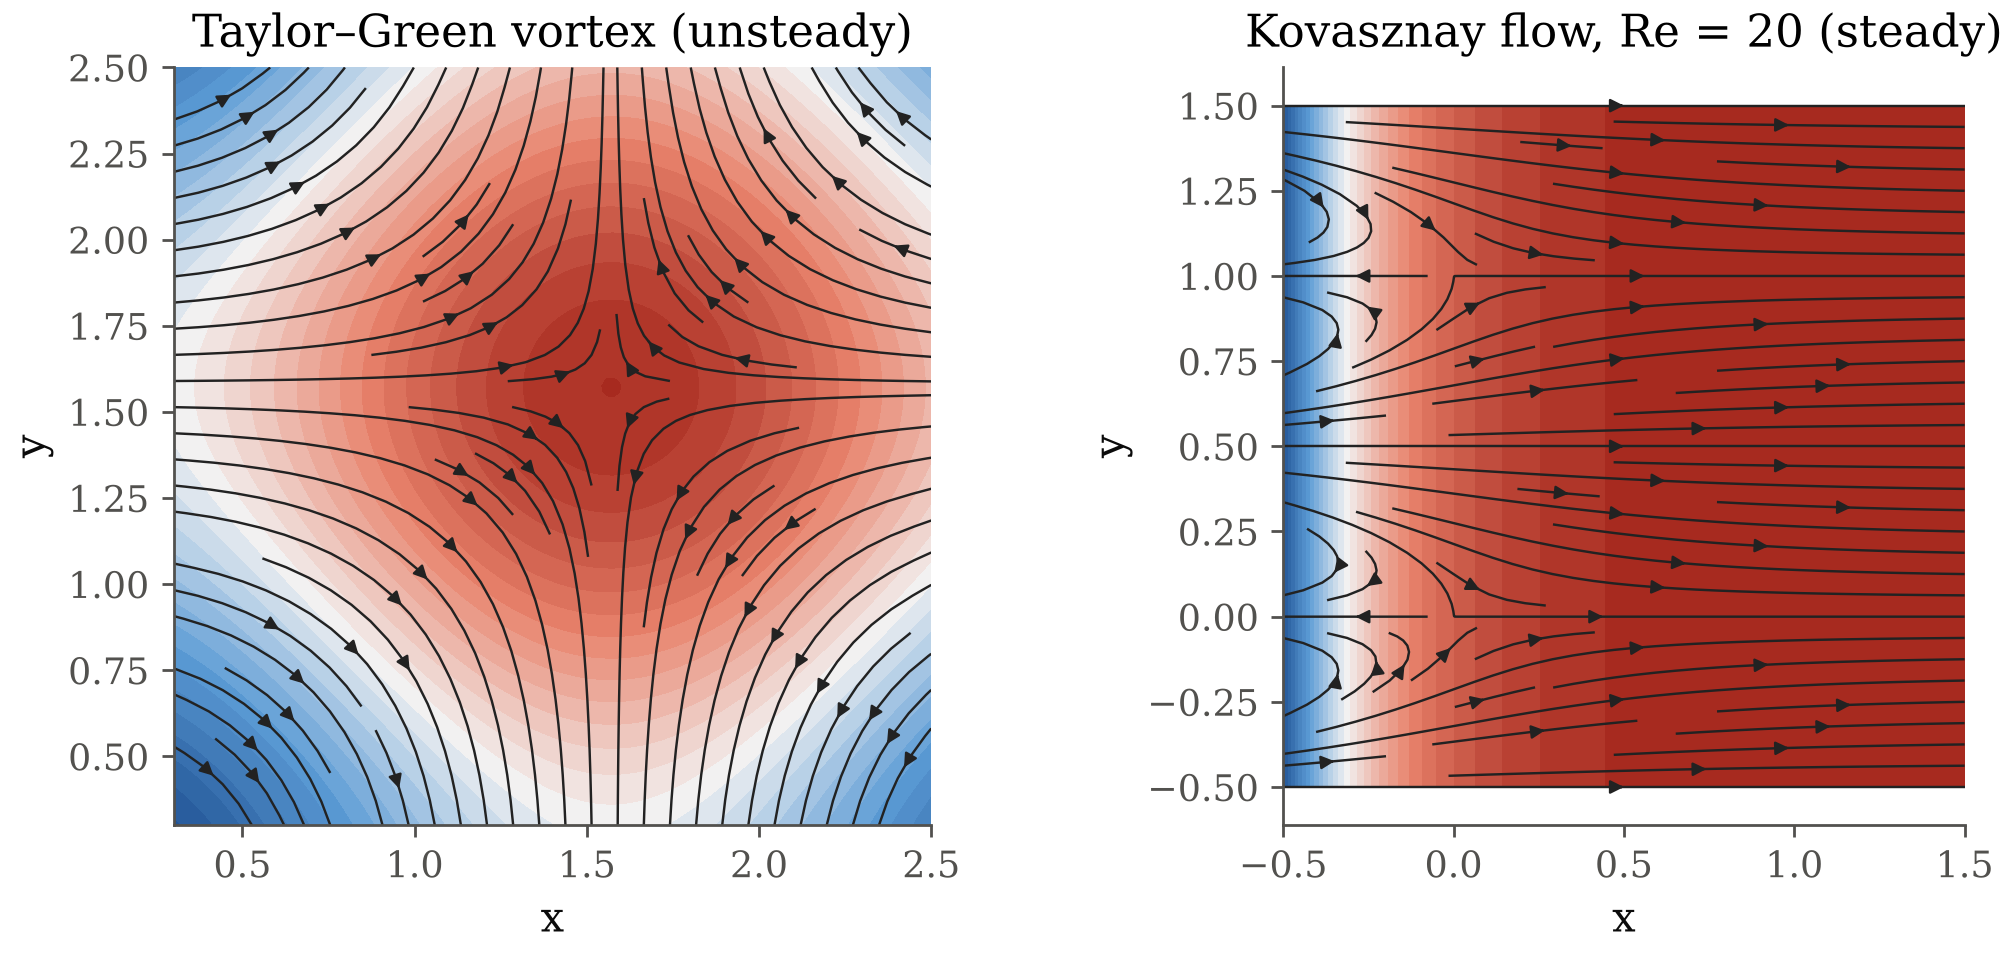
\includegraphics[width=0.85\linewidth]{img/f_testcases.png}
\caption{The two exact test flows: pressure (colour) and streamlines. Left: Taylor--Green on the window $[0.3,2.5]^2$. Right: Kovasznay flow at Re = 20 on $[-0.5,1.5]^2$.}\end{figure}

\section{Taylor--Green vortex}
\begin{equation}
u=\cos x\sin y\,F(t),\quad v=-\sin x\cos y\,F(t),\quad p=-\tfrac{\rho}{4}(\cos2x+\cos2y)F(t)^2,\quad F=e^{-2\nu t}.
\end{equation}
\textbf{Why it is exact.} Each velocity component is an eigenfunction of the Laplacian, $\nabla^2u=-2u$, so $\partial\uu/\partial t=-2\nu\uu=\nu\nabla^2\uu$: the unsteady and viscous terms cancel exactly. The convective term is then a pure gradient, balanced by $-\nabla p/\rho$:
\[
(\uu\cdot\nabla)\uu=\tfrac12\big(\sin2x,\;\sin2y\big)F^2=-\nabla p/\rho .
\]
So $\G=\nabla p$ comes entirely from convection: a good test of the convective term.

\textbf{Settings.} $\nu=0.01$, snapshots at $t=1\pm\Delta t$ with $\Delta t=0.05$.
\begin{itemize}
\item \textbf{Main window} $[0.3,2.5]^2$: deliberately non-periodic, so the Neumann boundary treatment is actually tested (on a full period the boundary terms would cancel).
\item \textbf{Core window} $[\pi-1.1,\pi+1.1]^2$: the main window contains no vortex core (its centre is a saddle, a pressure maximum), so vortex-core metrics use this second window centred on the core at $(\pi,\pi)$.
\end{itemize}

\textbf{Convected Taylor--Green.} Navier--Stokes is Galilean invariant: if $(\uu,p)$ is a solution, so is $\uu'(\mathbf x,t)=\mathbf c+\uu(\mathbf x-\mathbf ct,t)$, $p'=p(\mathbf x-\mathbf ct,t)$. With amplitude $A=0.4$ and $\mathbf c=(1,0)$ the vortex pattern is swept through the window, so $\partial\uu/\partial t=O(1)$ as in a real wake. This is the case where the Eulerian/Lagrangian comparison is meaningful (vortex speed $w=0.4$ < convection speed $c=1$).

\section{Kovasznay flow}
Kovasznay (1948) found an exact steady solution resembling the flow behind a grid:
\begin{equation}
u=1-e^{\lambda x}\cos2\pi y,\quad v=\frac{\lambda}{2\pi}e^{\lambda x}\sin2\pi y,\quad p=\frac{\rho}{2}\left(1-e^{2\lambda x}\right),\quad \lambda=\frac{Re}{2}-\sqrt{\frac{Re^2}{4}+4\pi^2}.
\end{equation}
\begin{itemize}
\item Continuity: $u_x=-\lambda e^{\lambda x}\cos2\pi y$ and $v_y=\lambda e^{\lambda x}\cos2\pi y$ cancel. \checkmark
\item Substituting into the steady equations gives $\lambda^2-Re\,\lambda-4\pi^2=0$; the negative root gives a wake that decays downstream: $\lambda\approx-1.81$ at Re = 20 and $-0.96$ at Re = 40.
\item The flow is steady, so $D\uu/Dt=(\uu\cdot\nabla)\uu$, and $\mu=\rho/Re$ is large: the viscous term matters. Kovasznay therefore tests the viscous term, which Taylor--Green does not.
\item Its pressure depends on $x$ only, with a steep gradient near the inflow edge $x=-0.5$.
\end{itemize}

\section{The synthetic PIV model}
\code{piv/degrade.py} turns an exact field into PIV-like data in three steps, applied in this order:
\begin{enumerate}
\item \textbf{Interrogation-window averaging.} The truth is sampled 4$\times$ finer than the PIV grid (with a margin), and a box filter of width $W$ is applied to $u$ and $v$ of every snapshot. For even widths the plain moving average would be off-centre by half a cell; the code averages the two half-shifted windows, which gives a centred trapezoidal box of width exactly $W$.
\item \textbf{Subsampling} to the PIV spacing $h$ (every 4th fine node), then cropping the margin, so the PIV nodes are exactly \code{linspace(x0, x1, n)}.
\item \textbf{Noise.} Independent Gaussian noise $N(0,(\sigma U)^2)$ on $u$ and $v$ at every node and snapshot, with a fixed seed.
\end{enumerate}
The \emph{reference pressure is never filtered}: it is only subsampled, so the measured error includes the bias that window averaging causes.

\textbf{Baseline.} $64\times64$ vectors, $W=h$, $\sigma=1\,\%$ of $U$, $\Delta t=0.05$. Each study varies one parameter around this baseline.

\begin{pitfall}[Fixed noise level across window sizes]
In real PIV a larger window contains more particles, so its random error is \emph{smaller}. The model keeps $\sigma$ fixed (as the project specification asked), so here $W$ only adds bias. Making $\sigma$ decrease with $W$ would reproduce the real resolution--noise trade-off; this is listed as future work.
\end{pitfall}

\section{Denoising}
Two optional filters act on $u$ and $v$ before differentiation:
\begin{itemize}
\item \textbf{Gaussian filter} (standard deviation 1 grid point): transfer function $e^{-(k s h)^2/2}$. It smooths everything, including real curvature.
\item \textbf{2-D Savitzky--Golay} ($5\times5$ window, quadratic): at each node, a least-squares fit of a polynomial in $x,y$, evaluated at the node (via the pseudo-inverse of the Vandermonde matrix). It reproduces quadratics exactly, also at the edges where the window is shifted inwards, so it biases smooth peaks less than the Gaussian.
\end{itemize}

\section{Error metrics}
Pressure is known only up to a constant, so both fields are demeaned first ($p'=p-\bar p$):
\begin{equation}
\eps_{L2}=\frac{\|p'-p'_{ref}\|_2}{\|p'_{ref}\|_2},\qquad
\eps_{max}=\frac{\max|p'-p'_{ref}|}{\tfrac12\rho U^2}.
\end{equation}
Also reported: the error map $|p'-p'_{ref}|$; a line profile through the vortex core; and the \textbf{core ratio}, reconstructed core pressure (minimum within $3h$ of the true core) divided by the true one. A ratio below 1 means the suction is under-predicted.

\section{Experiment design}
\begin{itemize}
\item \textbf{One factor at a time} around the baseline, so each effect is attributed cleanly (a local sensitivity study).
\item \textbf{Ten noise seeds} per point; results are mean $\pm$ standard deviation. The standard error of the mean falls as $1/\sqrt N$.
\item \textbf{Common random numbers:} the same seeds are reused across parameter values, so differences between parameter values are less noisy than the scatter itself.
\item Runs are deterministic: re-running reproduces every number.
\end{itemize}

% ------------------------------------------------------------------
\chapter{The code}

\section{Architecture}
\begin{figure}[H]
\centering
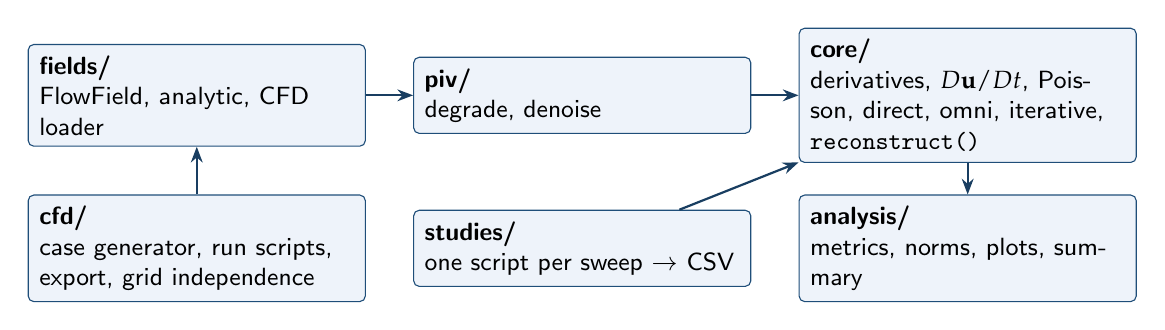
\begin{tikzpicture}[node distance=4mm and 6mm, every node/.style={font=\small\sffamily},
  mod/.style={draw=accent,fill=boxbg,rounded corners=2pt,align=left,text width=40mm,minimum height=9mm,inner sep=4pt},
  ar/.style={-{Stealth[length=2mm]},thick,color=accent!80!black}]
\node[mod] (fields) {\textbf{fields/}\\ FlowField, analytic, CFD loader};
\node[mod,right=of fields] (piv) {\textbf{piv/}\\ degrade, denoise};
\node[mod,right=of piv] (core) {\textbf{core/}\\ derivatives, $D\uu/Dt$, Poisson, direct, omni, iterative, \code{reconstruct()}};
\node[mod,below=of core] (an) {\textbf{analysis/}\\ metrics, norms, plots, summary};
\node[mod,left=of an] (st) {\textbf{studies/}\\ one script per sweep $\to$ CSV};
\node[mod,left=of st] (cfd) {\textbf{cfd/}\\ case generator, run scripts, export, grid independence};
\draw[ar] (fields)--(piv); \draw[ar] (piv)--(core); \draw[ar] (core)--(an); \draw[ar] (st)--(core); \draw[ar] (cfd)--(fields);
\end{tikzpicture}
\caption{Package structure. Every data source returns a \code{FlowField}; every algorithm consumes one.}
\end{figure}

\begin{itemize}
\item \textbf{\code{FlowField}} (\code{fields/field.py}) is the common interface: $x,y,t$ and arrays $u,v$ of shape $[n_t,n_y,n_x]$, plus $\rho$, $\mu$, the reference pressure and $U_{ref}$. It checks that the grids are uniform, because every stencil assumes constant spacing.
\item \textbf{\code{reconstruct()}} (\code{core/pipeline.py}) is the single entry point: it computes $\G$, then calls the chosen method, and returns the pressure plus diagnostics (compatibility residual, timings, solver history).
\item \textbf{\code{studies/}} contains one script per parameter sweep; each writes a CSV row per reconstruction and saves its figures.
\item \textbf{\code{analysis/summary.py}} writes \code{results/SUMMARY.md} from the CSVs, so no number in the report is typed by hand.
\end{itemize}

\section{Pseudo-code}
\begin{lstlisting}
for case in [TaylorGreen, ConvectedTG, Kovasznay20, Kovasznay40, CFD]:
    truth = exact_or_cfd(case)                 # u, v, p on a 4x finer grid
    for param in sweep(h | sigma | dt | BC | method | W | filter):
        for seed in range(10):
            F  = degrade(truth, W, h, sigma, seed)  # box filter, subsample, noise
            F  = denoise(F)                     # optional
            a  = DuDt(F, eulerian | lagrangian)
            G  = -rho*a + mu*lap(u)
            p  = poisson(G) | direct(G) | omni(G)
            eps  = L2(p' - p'_ref) / L2(p'_ref)   # p' = p - mean(p)
        save mean, std of eps -> CSV -> figures -> SUMMARY.md
\end{lstlisting}

\section{Inside the Poisson solve}
\begin{lstlisting}
f = div(G)                                  # or -rho(u_x^2 + 2 u_y v_x + v_y^2)
b = f + ghost-point terms +/-2G/h on the edges (both at corners)
R = trapz(f) - contour(n.G)                 # compatibility residual, reported
if Dirichlet edges:   rows -> p_k = value
elif pin == "node":   row k -> p_k = 0
else:                 solve [[A, 1], [1^T, 0]] [p, lam] = [b, 0]   # zero mean
p = spsolve(...)   or   Jacobi / GS / SOR / CG on the same system
\end{lstlisting}

\section{Tests: how we know the code is right}
87 unit tests (\code{python -m pytest -q}, about 15\,s) check every component against an exact answer:
\begin{itemize}
\item \textbf{Derivatives:} second-order slopes in the max norm, including boundary nodes; exact on quadratics and cubics.
\item \textbf{Poisson:} the manufactured solution $p=\sin x\cos y$ converges at order 2 for pin-mean, pin-node, direct and CG; the null space, $w^TA=0$, symmetry of $WA$, and the discrete compatibility identity.
\item \textbf{Taylor--Green and Kovasznay:} $\G=+\nabla p$ to second order; full reconstruction second order for all three methods; without $\mu\nabla^2\uu$ Kovasznay does not converge.
\item \textbf{Methods:} all exact for linear $p$; agree on clean data; noisy data show path dependence and omni/Poisson beat a single path.
\item \textbf{PIV model and I/O:} box filter centred and normalised; noise seeding; Savitzky--Golay preserves quadratics; OpenFOAM export parsers; Strouhal number from a synthetic force file; Richardson extrapolation recovers order 2.
\item \textbf{Convergence add-on:} norms (the lecture example), Jacobi = pseudo-time, classic-Jacobi stall, SOR divergence, all iterative solvers match \code{spsolve}, slope $\approx1$ for \code{order=1} and $\approx2$ for \code{order=2}.
\end{itemize}

\begin{viva}
\begin{enumerate}[leftmargin=*]
\item \emph{Why generate the truth finer than the PIV grid?} A PIV vector is an average over the window, so the underlying field must be resolved below $h$.
\item \emph{Why fixed seeds?} Reproducibility, and common random numbers make differences between parameter values less noisy.
\item \emph{How do you test second order?} Halve $h$ repeatedly and fit the slope of $\log\eps$ against $\log h$; the tests accept 1.8--2.3 because coarse grids are pre-asymptotic.
\item \emph{Why a common \code{FlowField}?} Degradation, integration and metrics need not know whether data are analytic, CFD or turbulence-database data.
\end{enumerate}
\end{viva}

% ================================================================== PART IV
\part{Results and what they mean}

\chapter{Reconstruction results}
All numbers are means over 10 noise seeds from \code{results/*.csv}. The baseline is $n=64$, $W=h$, $\sigma=1\,\%$, $\Delta t=0.05$, Poisson with all-Neumann edges and the zero-mean constraint, Eulerian $D\uu/Dt$.

\section{Verification: grid convergence on clean data}
First the code must be shown correct, with no noise and no window averaging (exact point samples).
\begin{figure}[H]\centering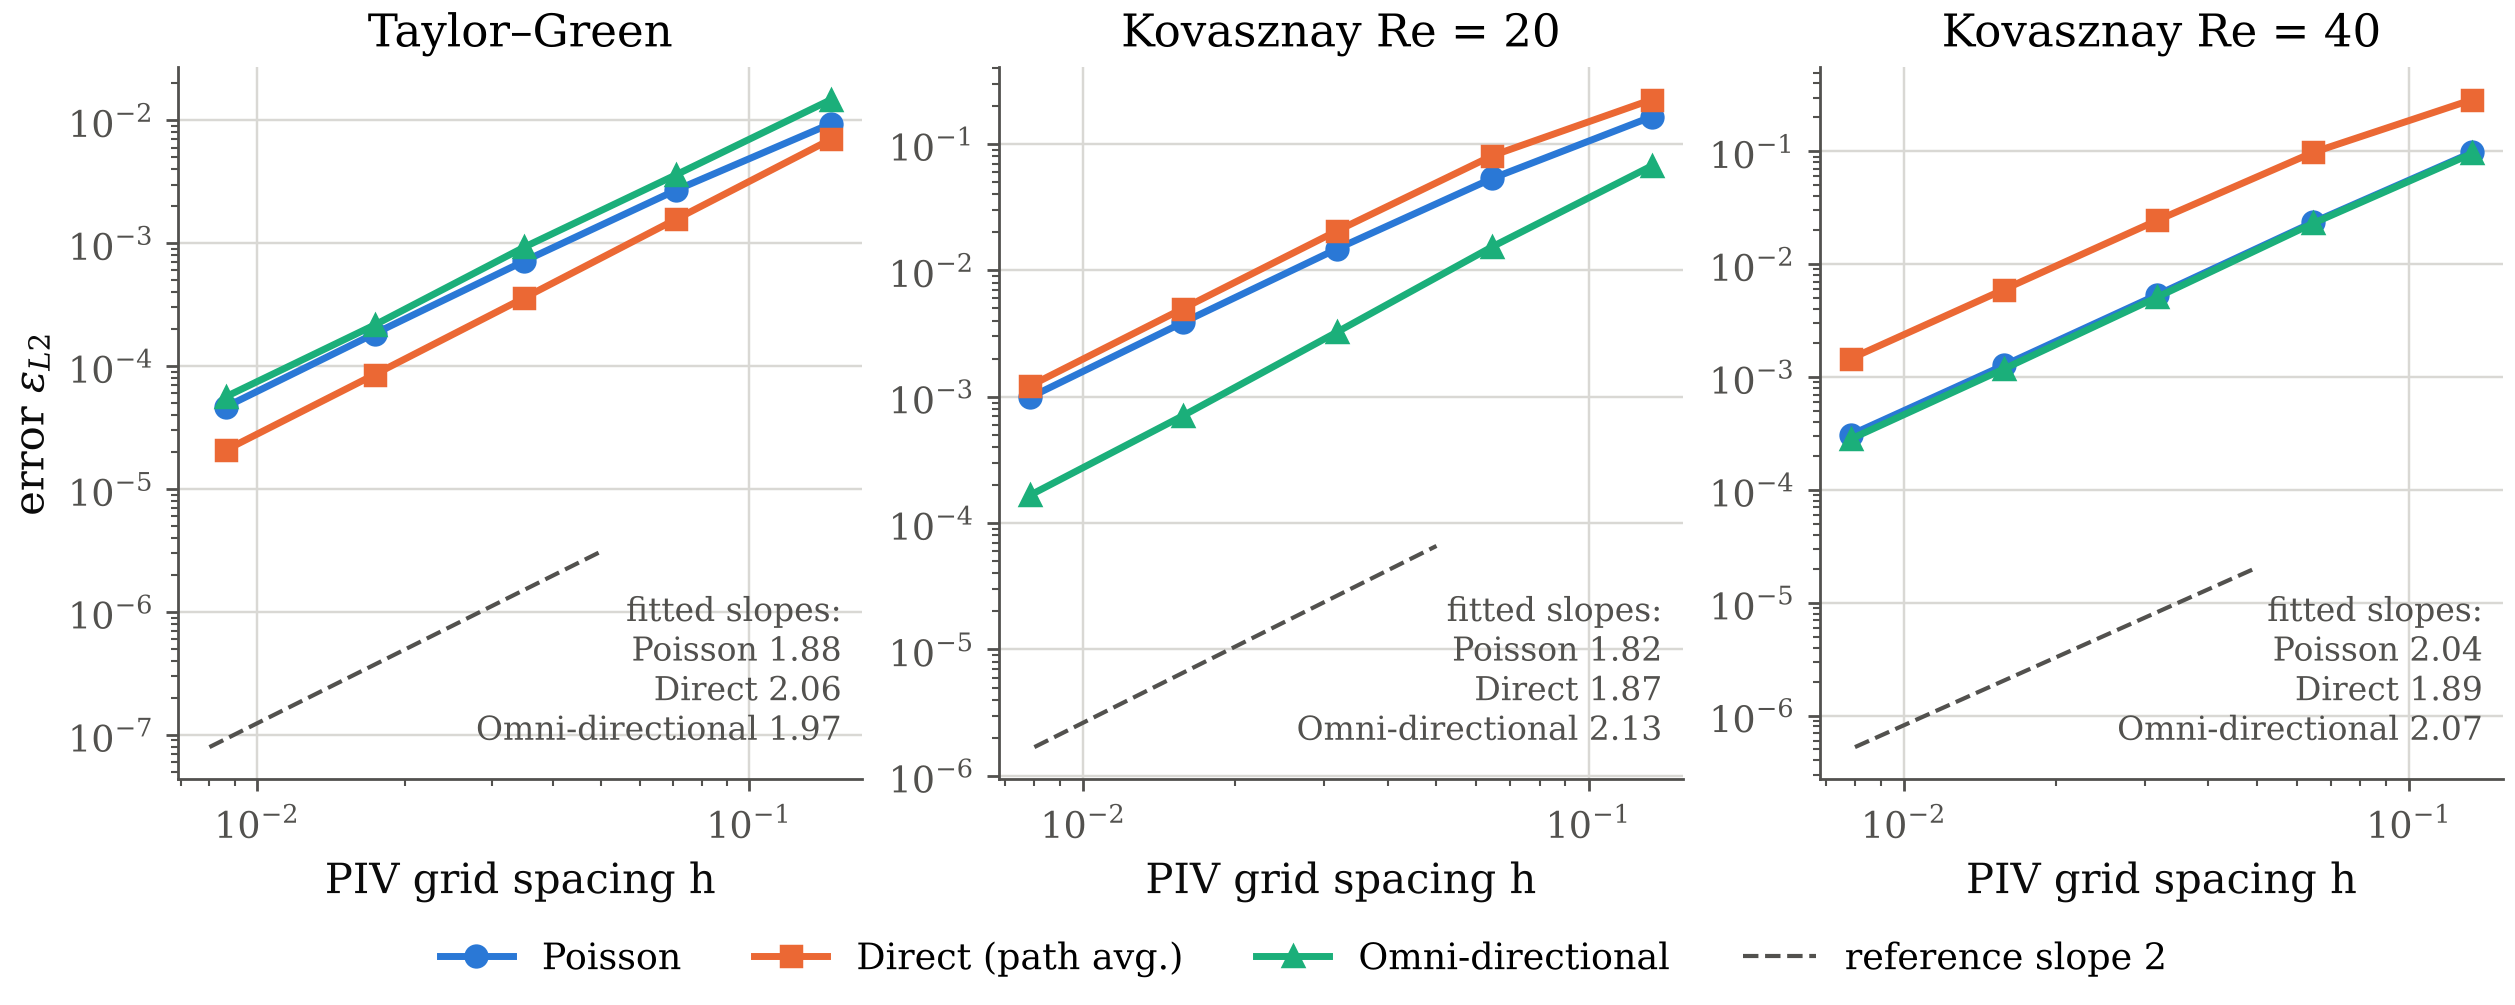
\includegraphics[width=\linewidth]{img/f_conv_clean.png}
\caption{Error vs PIV spacing on clean data for the three test flows and three methods; dashed line: slope 2.}\end{figure}

\begin{table}[H]\centering\small
\begin{tabular}{@{}lccc@{}}\toprule
Fitted slope of $\eps_{L2}$ vs $h$ ($16^2$--$256^2$) & Poisson & Direct & Omni\\\midrule
Taylor--Green & 1.88 & 2.06 & 1.97\\
Kovasznay Re = 20 & 1.82 & 1.87 & 2.13\\
Kovasznay Re = 40 & 2.04 & 1.89 & 2.07\\\bottomrule
\end{tabular}\end{table}

\textbf{What it shows.} All three methods are second-order accurate on all three flows, as the $O(h^2)$ stencils and trapezoidal rule predict. Between the two finest grids the local Poisson slopes are 1.96--2.03; fits over all grids are slightly lower because the coarsest grids are pre-asymptotic. The finest-grid errors are tiny ($4.7\times10^{-5}$ for Poisson on Taylor--Green at $256^2$). Kovasznay errors are larger at a given $h$ because its pressure varies steeply near the inflow edge ($e^{2\lambda x}$). The code is verified before any noise is added.

\section{Noise vs resolution: an optimum spacing}
\begin{figure}[H]\centering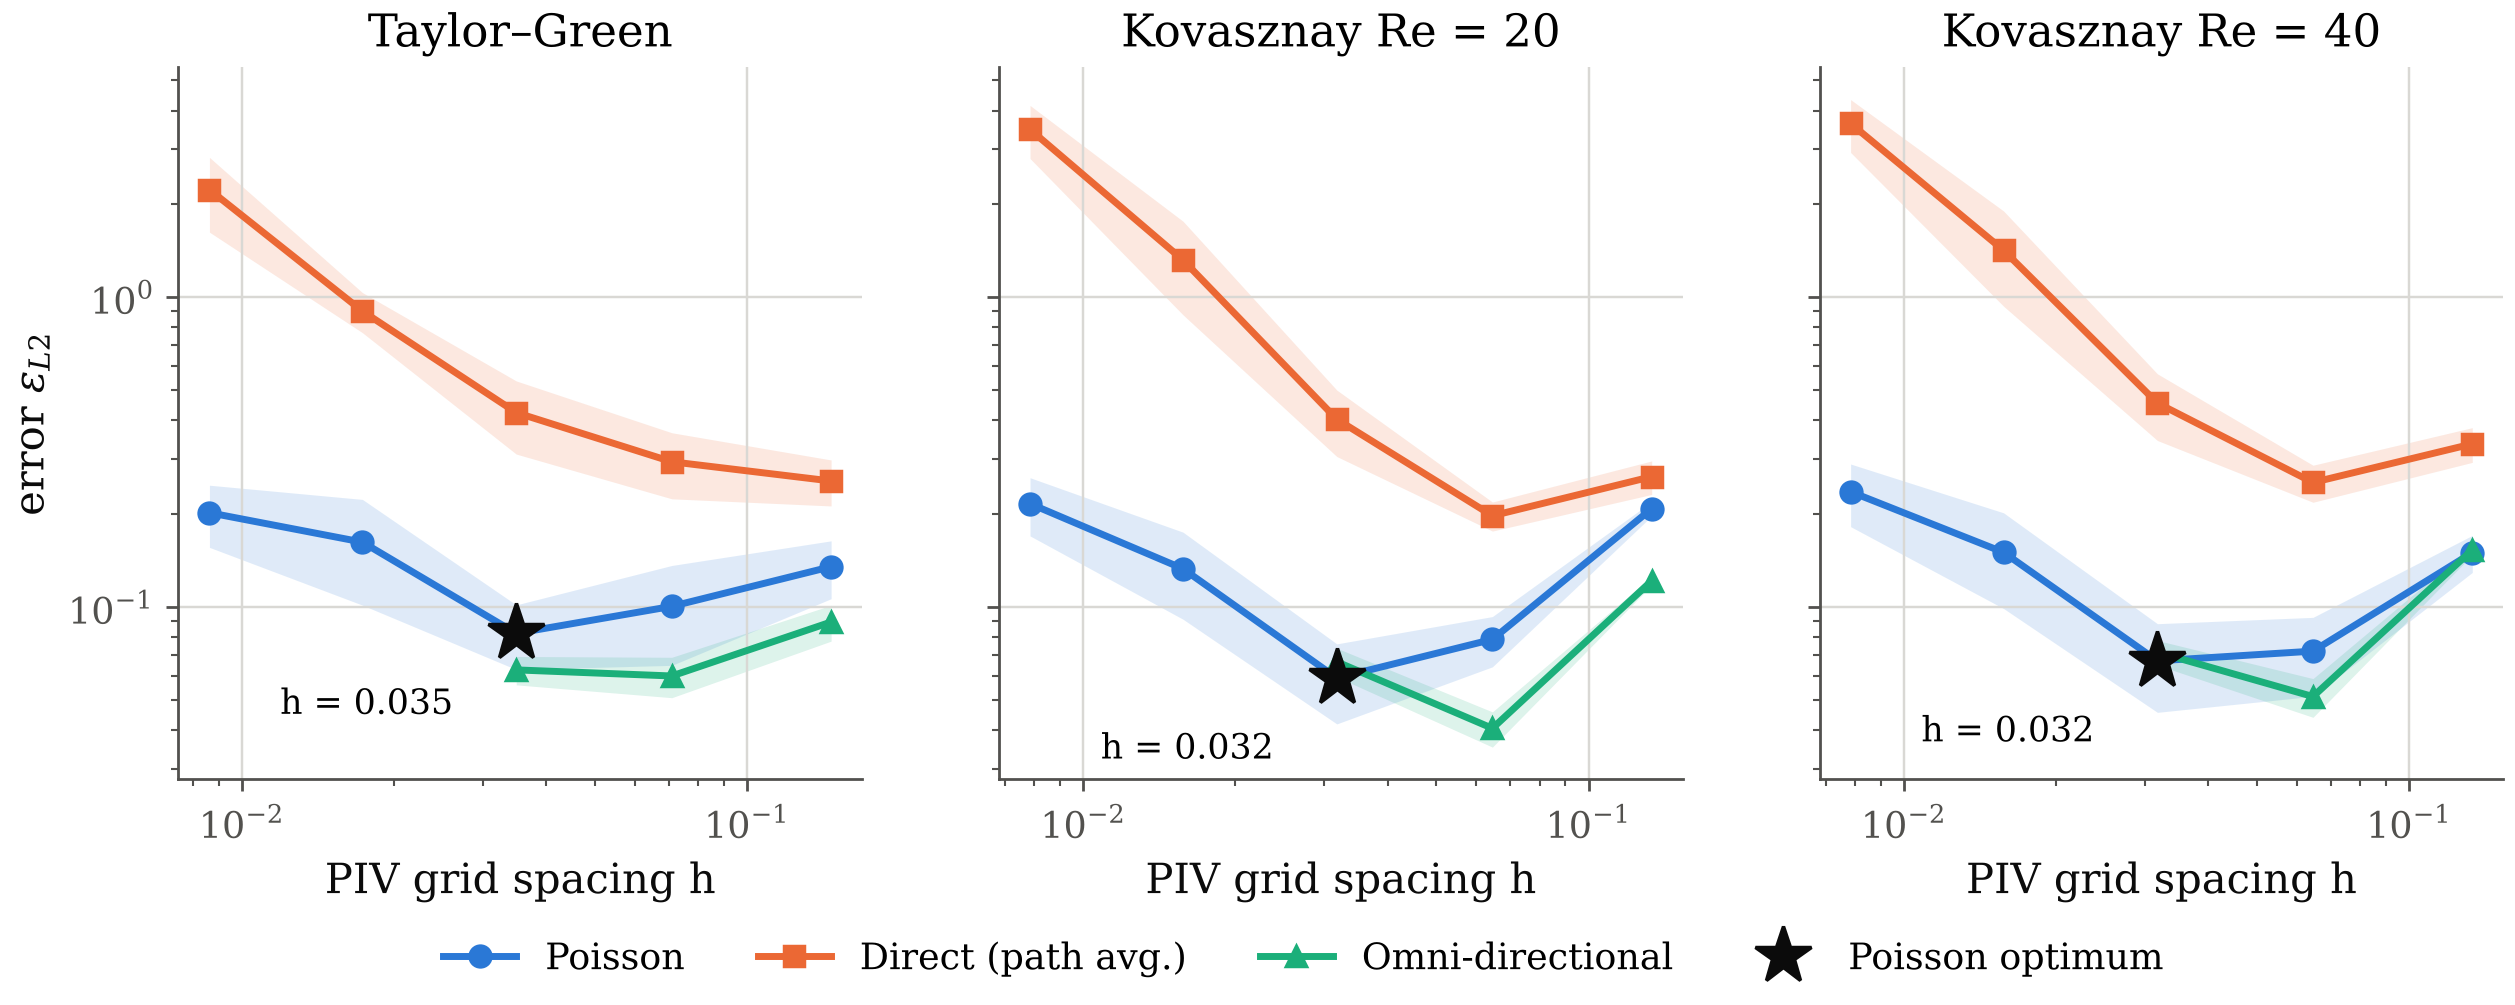
\includegraphics[width=\linewidth]{img/f_conv_noisy.png}
\caption{Error vs spacing with $\sigma=1\,\%$, $W=h$ (mean $\pm$ std of 10 seeds). Stars: the Poisson optimum.}\end{figure}

\begin{table}[H]\centering\small
\begin{tabular}{@{}rrccc@{}}\toprule
$n$ & $h$ (TG) & Taylor--Green & Kovasznay 20 & Kovasznay 40\\\midrule
16 & 0.147 & 0.135 & 0.208 & 0.150\\
32 & 0.071 & 0.101 & 0.079 & 0.072\\
\textbf{64} & \textbf{0.035} & \textbf{0.082} & \textbf{0.059} & \textbf{0.067}\\
128 & 0.017 & 0.162 & 0.133 & 0.150\\
256 & 0.009 & 0.202 & 0.216 & 0.236\\\bottomrule
\end{tabular}
\caption{Poisson $\eps_{L2}$ with 1\,\% noise. The minimum is at $n=64$ for all three flows.}\end{table}

\textbf{What it shows and why.} With noise, refining the grid stops helping: the Poisson error is lowest at $h\approx0.032$--$0.035$ ($n=64$) for all three flows and rises again on finer grids. This is the trade-off of Eq.~\eqref{eq:noiseG}. Truncation error falls as $h^2$, but noise is amplified as $\sigma/h$ by the convective term and as $\mu\sigma/h^2$ by the viscous term. At $h=0.035$ the viscous noise is already comparable to the convective noise, and it grows fastest.

\textbf{Direct integration only gets worse} as the grid is refined (Taylor--Green 0.26 $\to$ 2.2): a path crosses $\sim1/h$ noisy steps and its error grows like a random walk. On Kovasznay its optimum is at the coarser $h\approx0.065$.

\begin{keyidea}[Practical consequence]
For noisy PIV data there is a best vector spacing. Asking for the finest possible PIV grid can make the pressure \emph{worse}. The optimum moves to coarser grids as the noise level rises.
\end{keyidea}

\section{Noise sensitivity and choice of method}
\begin{figure}[H]\centering
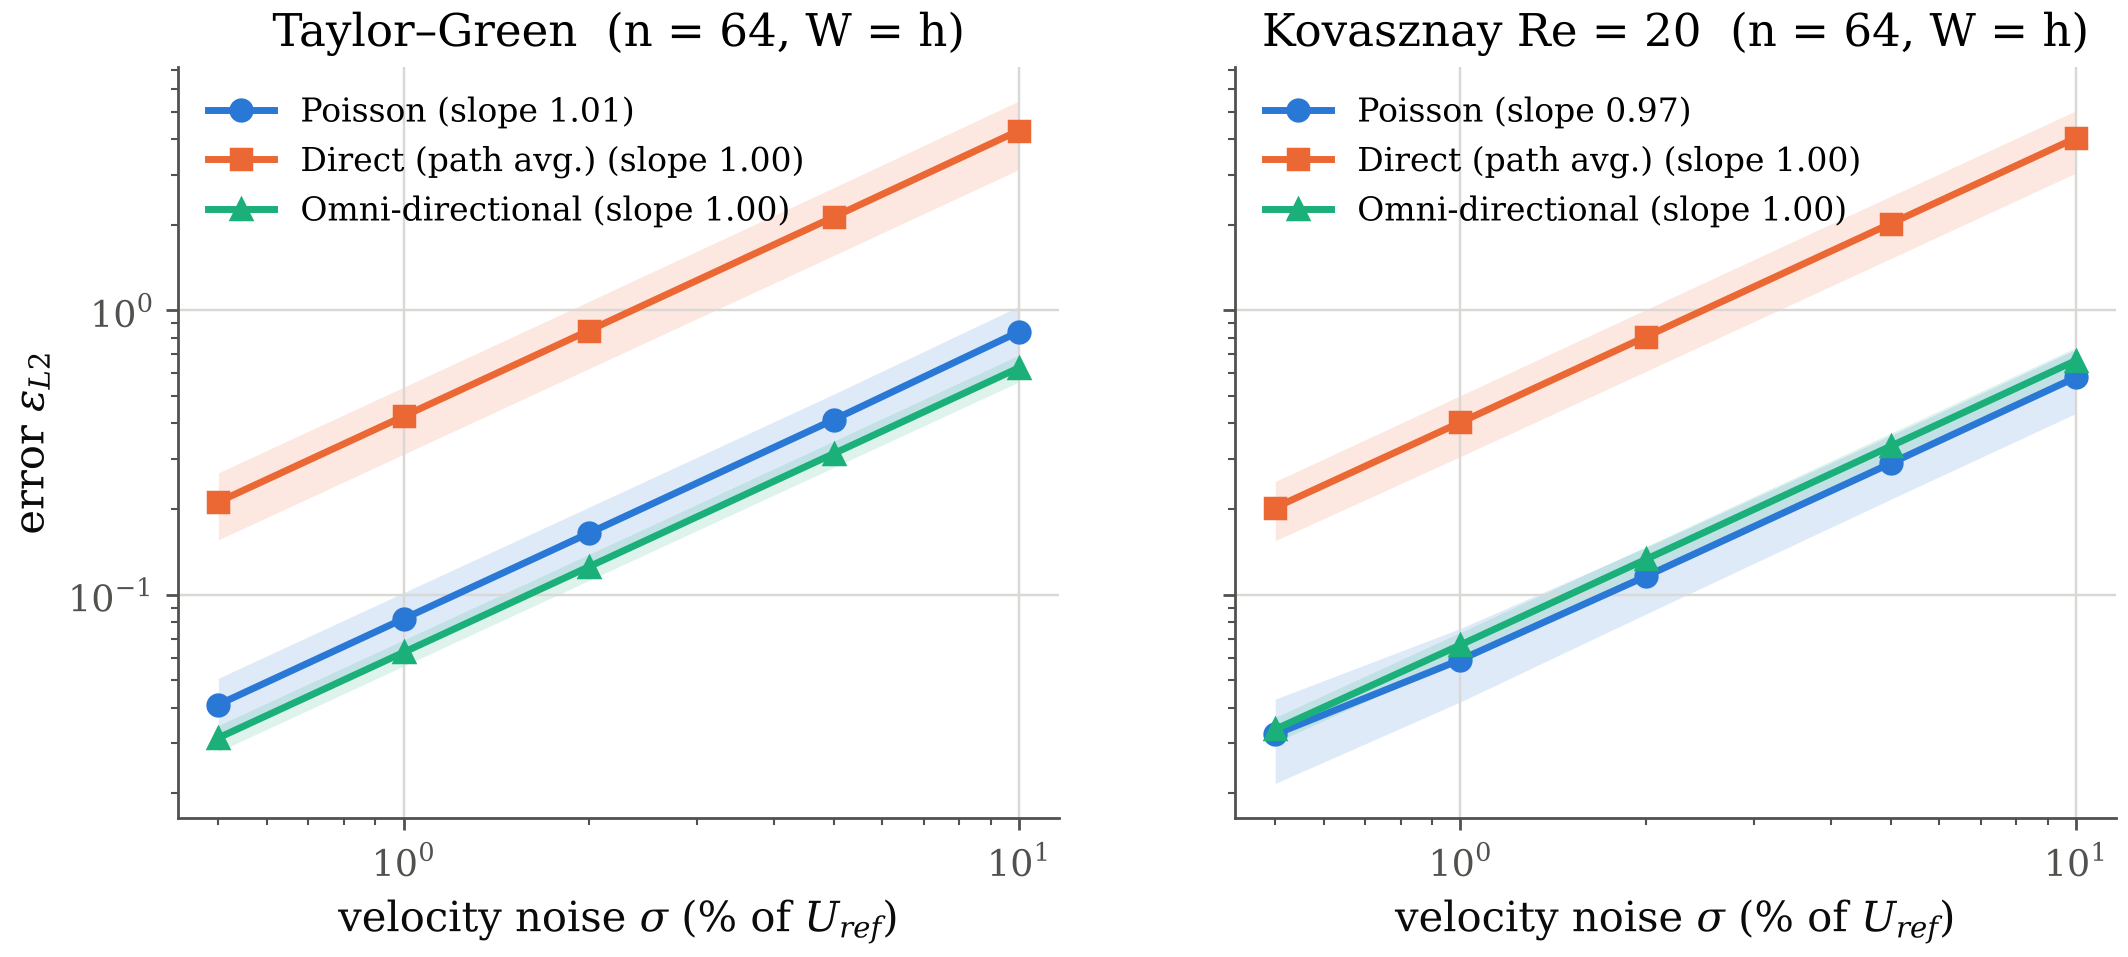
\includegraphics[width=0.85\linewidth]{img/f_noise.png}
\caption{Error vs noise level ($n=64$, $W=h$); the slopes in the legend are log--log fits.}\end{figure}
\begin{figure}[H]\centering
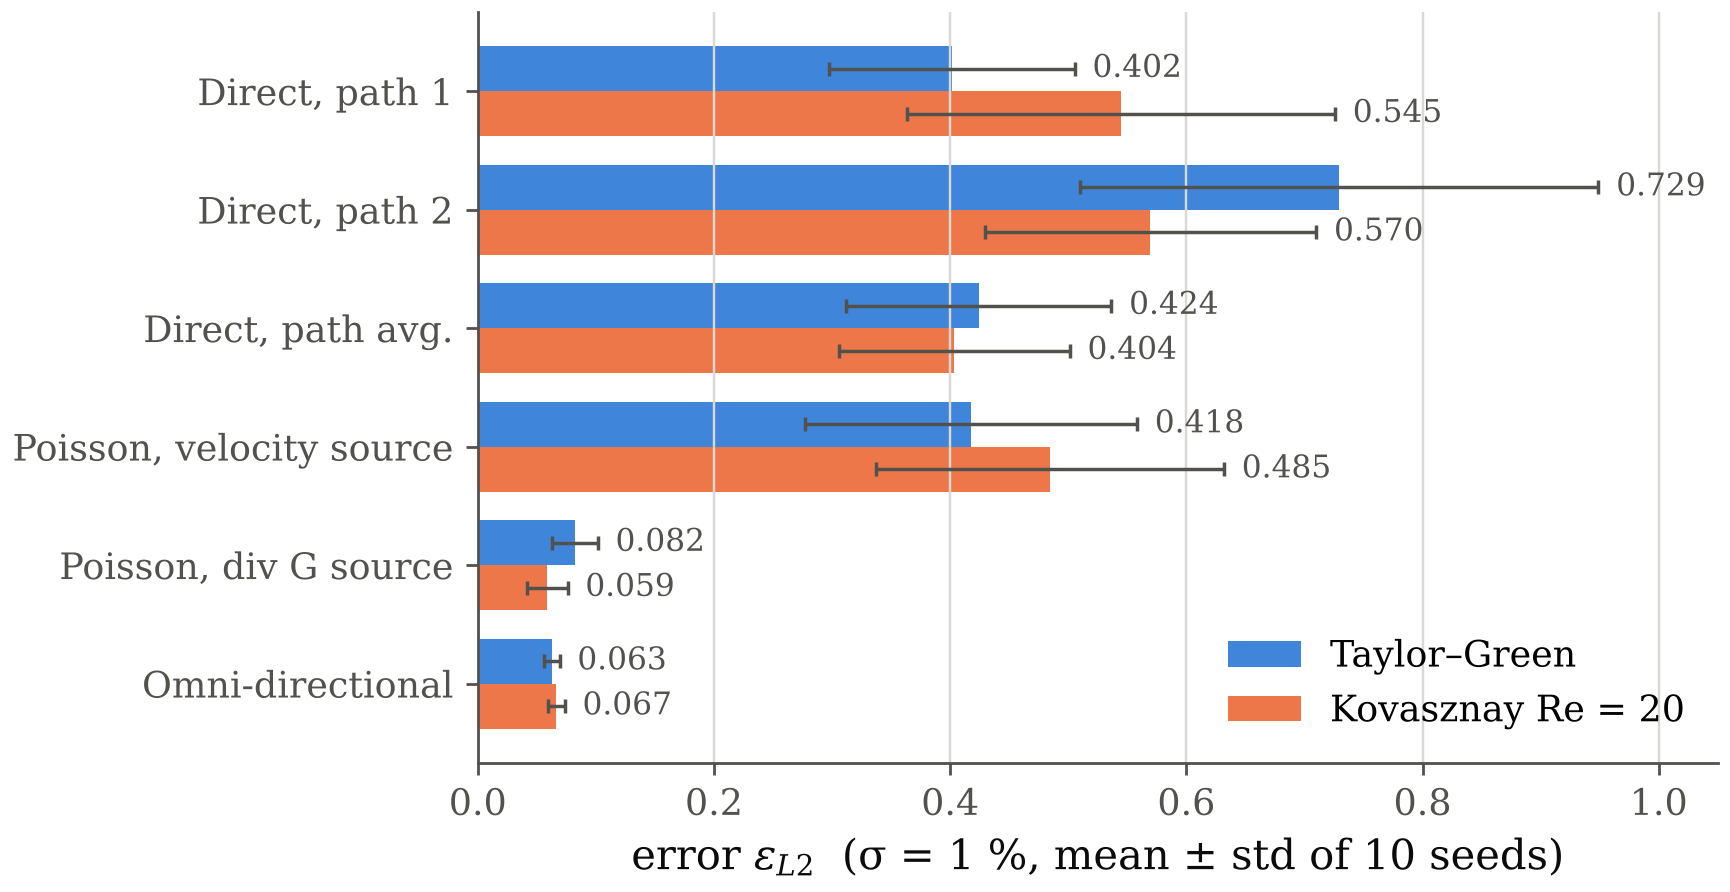
\includegraphics[width=0.62\linewidth]{img/f_method_bar.png}
\caption{All integration variants at $\sigma=1\,\%$ (mean $\pm$ std of 10 seeds).}\end{figure}

\begin{table}[H]\centering\small
\begin{tabular}{@{}lccccc@{}}\toprule
 & \multicolumn{2}{c}{$\eps_{L2}$ at $\sigma=1\,\%$} & \multicolumn{2}{c}{log--log slope vs $\sigma$} & Time per\\
Method & TG & Kov 20 & TG & Kov 20 & reconstruction\\\midrule
Direct (path avg.) & 0.424 & 0.404 & 1.00 & 1.00 & 0.3 ms\\
Poisson ($\nabla\cdot\G$ source) & 0.082 & 0.059 & 1.01 & 0.97 & 15 ms\\
Omni-directional & 0.063 & 0.067 & 1.00 & 1.00 & 0.41 s\\
Poisson (velocity source) & 0.418 & 0.485 & -- & -- & 15 ms\\\bottomrule
\end{tabular}\end{table}

\begin{enumerate}
\item \textbf{Error grows linearly with noise} (log--log slopes 0.97--1.01). The whole reconstruction is a linear operation on the velocity error (apart from the small quadratic convective term), so doubling the noise doubles the error.
\item \textbf{Direct integration is 5--7$\times$ worse.} A single path carries every error along it; Poisson (elliptic: every point sees the whole domain) and omni (average of 32 directions) average errors out.
\item \textbf{Omni and Poisson are equally accurate} (each wins one flow) but omni is about 27$\times$ slower. Poisson is the practical choice.
\item \textbf{Path 1 and path 2 differ} (Taylor--Green 0.40 vs 0.73). This is not a bug: mirroring the data ($x\leftrightarrow y$) swaps the two errors exactly. Noise in the convective and viscous terms comes from the same snapshot, so the terms are correlated; whether they add or cancel along a path depends on the flow direction relative to the path.
\item \textbf{The velocity-source Poisson form is 5--8$\times$ worse with noise.} Its interior source multiplies noisy derivatives, while its boundary data still come from $\G$, so source and boundary data no longer come from one vector field. The least-squares structure of Section~3.3.2 is lost. (With noise-free boundary data it was actually better: its weakness is the mismatch, not the identity.)
\end{enumerate}

\begin{figure}[H]\centering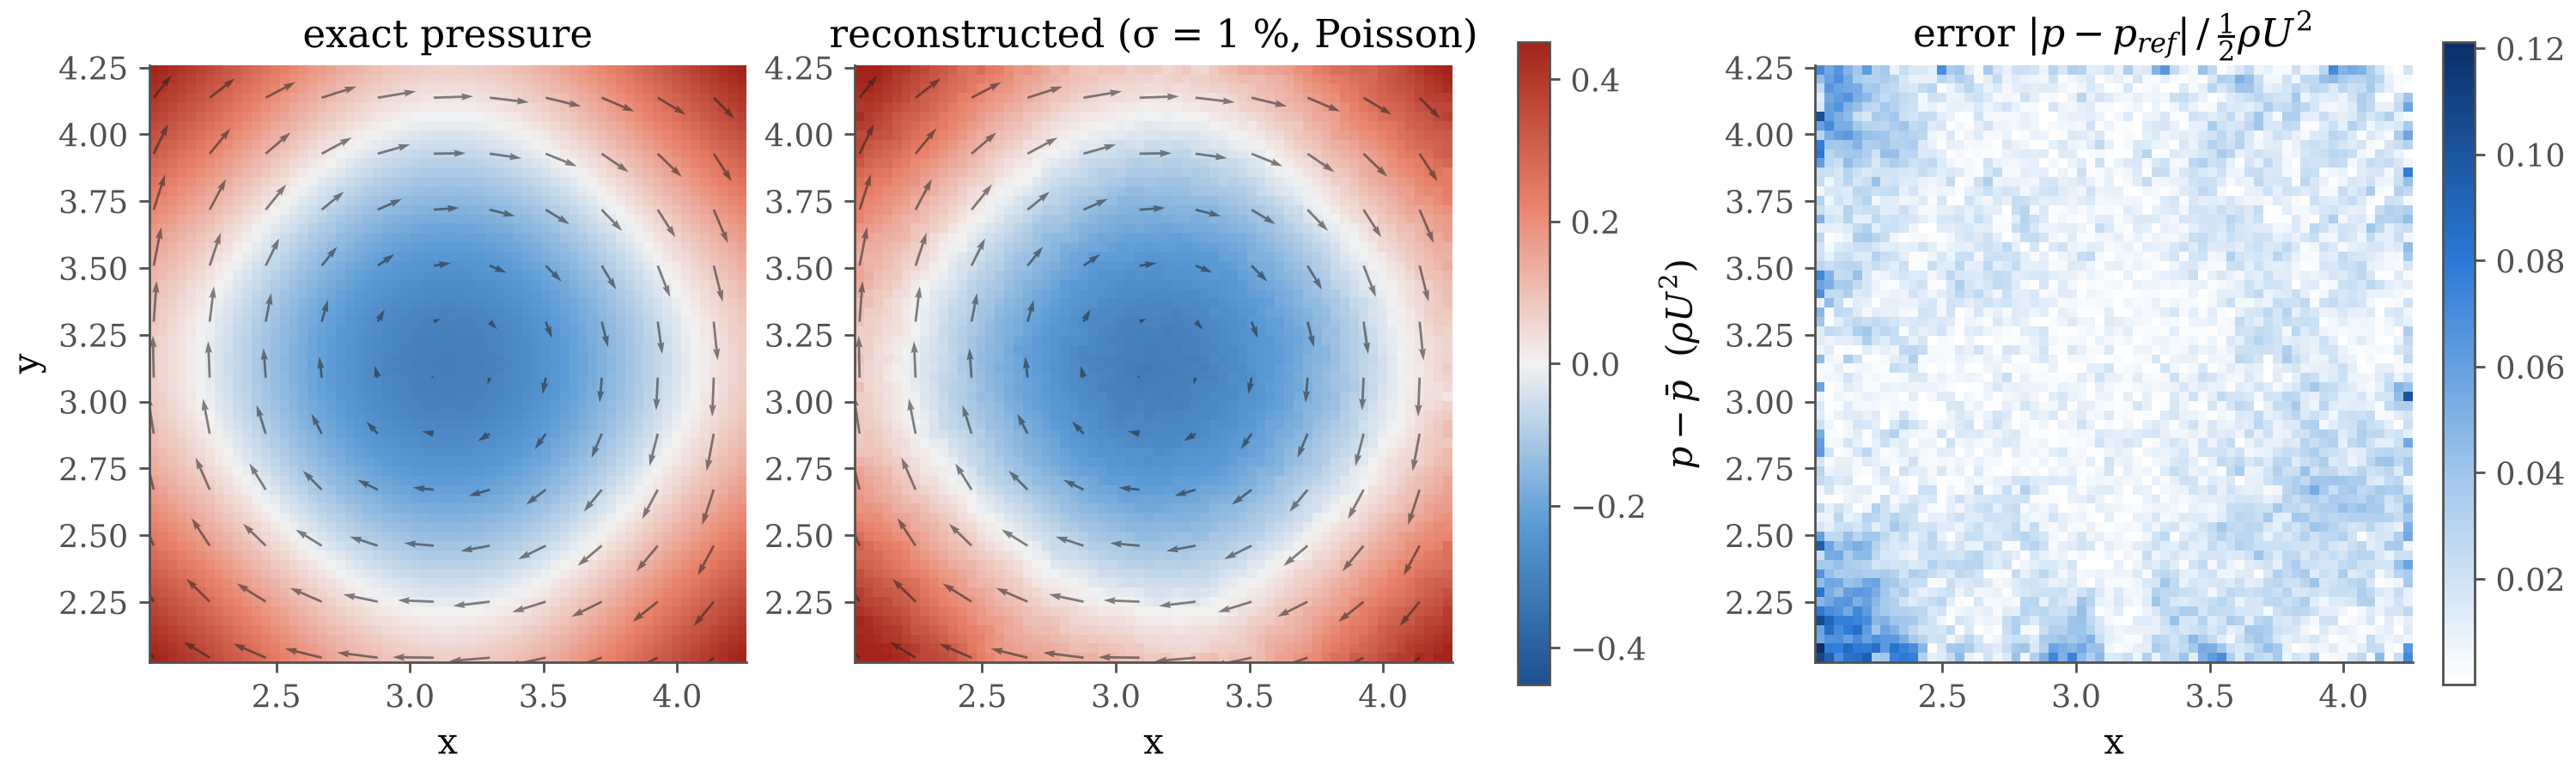
\includegraphics[width=\linewidth]{img/f_fields_tg.png}
\caption{Taylor--Green core window: exact pressure, reconstruction from noisy PIV-like data ($\sigma=1\,\%$, Poisson, $\eps_{L2}=0.061$ for this seed), and the error map. The vortex is recovered; the error is mostly random scatter, largest at the edges.}\end{figure}

\section{Boundary conditions for the Poisson solver}
\begin{figure}[H]\centering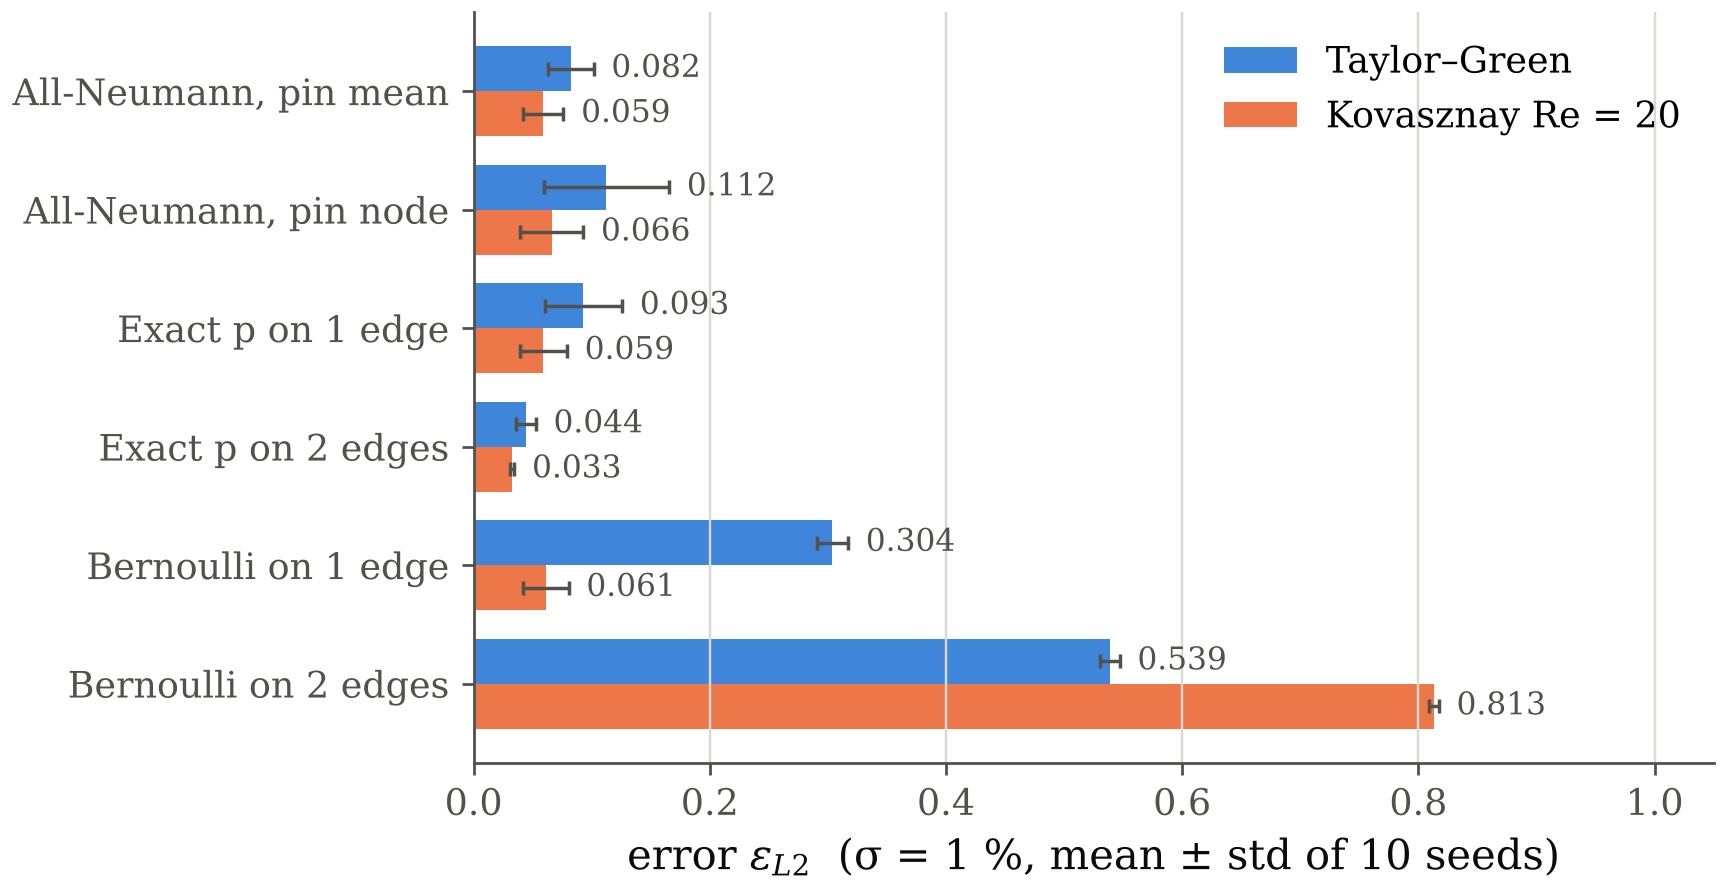
\includegraphics[width=0.62\linewidth]{img/f_bc_bar.png}
\caption{Poisson error for six boundary treatments at $\sigma=1\,\%$.}\end{figure}

\begin{table}[H]\centering\small
\begin{tabular}{@{}lcc@{}}\toprule
Boundary treatment & TG noisy $\eps_{L2}$ & Kov 20 noisy $\eps_{L2}$\\\midrule
All-Neumann, zero mean (baseline) & 0.082 & 0.059\\
All-Neumann, pin one node & 0.112 & 0.066\\
Exact $p$ on 1 edge & 0.093 & 0.059\\
\textbf{Exact $p$ on 2 opposite edges} & \textbf{0.044} & \textbf{0.033}\\
Bernoulli on 1 edge & 0.304 & 0.061\\
Bernoulli on 2 edges & 0.539 & 0.813\\\bottomrule
\end{tabular}\end{table}

\begin{enumerate}
\item \textbf{Known pressure on two opposite edges halves the error.} Neumann data $\n\cdot\G$ are themselves noisy derivatives, so their errors propagate inward; a Dirichlet edge anchors the solution. Two opposite edges bracket the domain. (The ``exact'' option is an oracle standing in for wall pressure taps.)
\item \textbf{One edge helps little or even hurts}: the Neumann-data error is anchored on one side only and accumulates across the domain.
\item \textbf{Pinning a node is worse than the zero-mean constraint}: it dumps the incompatibility at one point (Section~5.3).
\item \textbf{Bernoulli edges fail} (up to 0.81): $p+\tfrac12\rho|\uu|^2=$ const holds only in irrotational flow, and both flows are rotational everywhere. Use Bernoulli only at genuine free-stream edges.
\end{enumerate}

\section{Time step: Eulerian vs Lagrangian}
\begin{figure}[H]\centering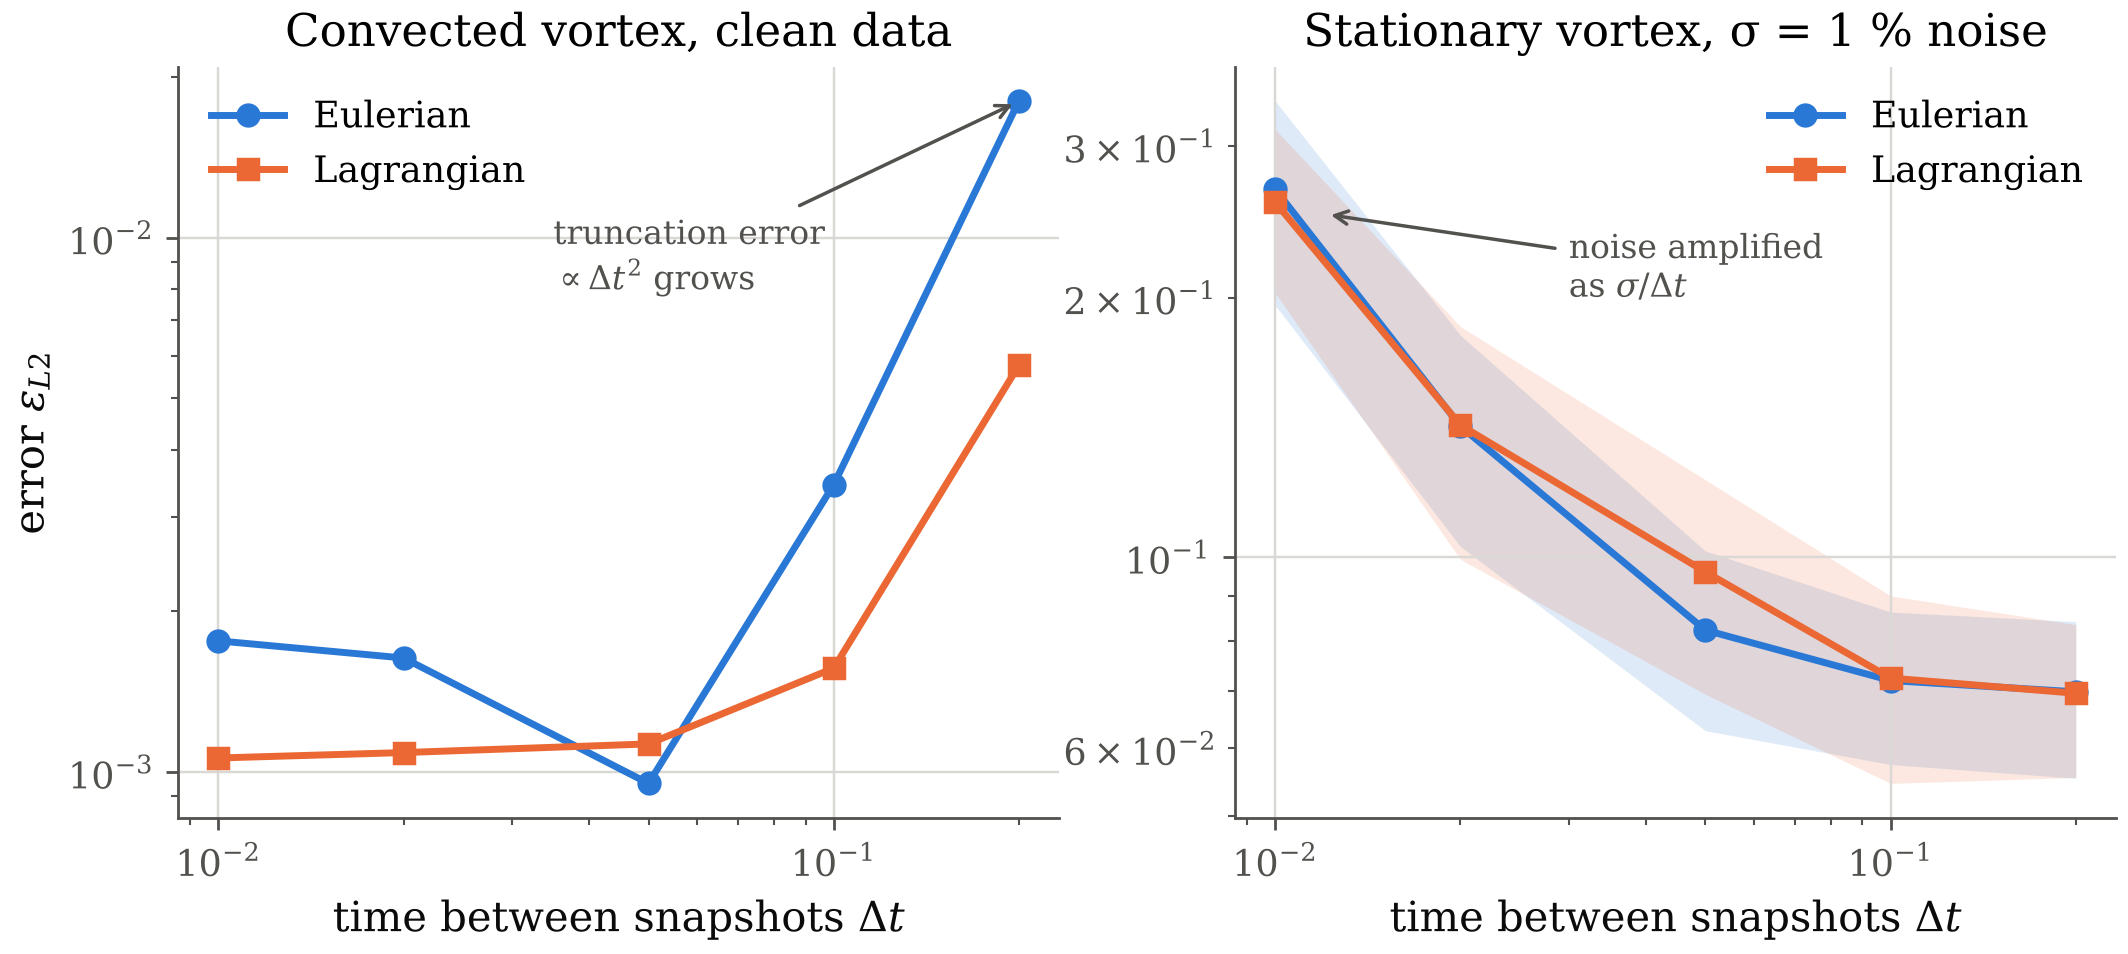
\includegraphics[width=0.85\linewidth]{img/f_dt.png}
\caption{Error vs time between snapshots. Left: convected vortex, clean data. Right: stationary vortex with 1\,\% noise.}\end{figure}

\begin{table}[H]\centering\small
\begin{tabular}{@{}rcccc@{}}\toprule
 & \multicolumn{2}{c}{Convected TG, clean} & \multicolumn{2}{c}{Stationary TG, $\sigma=1\,\%$}\\
$\Delta t$ & Eulerian & Lagrangian & Eulerian & Lagrangian\\\midrule
0.01 & $1.8\times10^{-3}$ & $1.1\times10^{-3}$ & 0.267 & 0.258\\
0.05 & $9.5\times10^{-4}$ & $1.1\times10^{-3}$ & 0.082 & 0.096\\
0.10 & $3.5\times10^{-3}$ & $1.6\times10^{-3}$ & 0.072 & 0.072\\
0.20 & $1.8\times10^{-2}$ & $5.8\times10^{-3}$ & 0.070 & 0.070\\\bottomrule
\end{tabular}\end{table}

\begin{enumerate}
\item \textbf{Convected vortex (clean):} the Eulerian error grows 10$\times$ from $\Delta t=0.01$ to 0.2, because at a fixed point the pattern sweeps past and $\partial\uu/\partial t$ changes quickly ($\propto c^3$). The Lagrangian scheme follows the particle; its error grows only with the vortex's own velocity ($\propto w^3$) and is 3$\times$ lower at $\Delta t=0.2$. This is exactly the $w/c$ argument of Section~3.2.
\item \textbf{Stationary vortex (clean):} the Eulerian error does not depend on $\Delta t$ (the flow barely changes at a point), while the Lagrangian error grows (to $4.2\times10^{-3}$ at $\Delta t=0.2$) because it traces curved particle paths with a straight step.
\item \textbf{Noisy data:} both schemes \emph{improve} with larger $\Delta t$ (0.27 $\to$ 0.07), because the noise in $\partial\uu/\partial t$ scales as $\sigma/\Delta t$ and dominates over this range. The best $\Delta t$ balances noise against truncation error, just like the best $h$.
\end{enumerate}

\section{Interrogation window and denoising}
\begin{figure}[H]\centering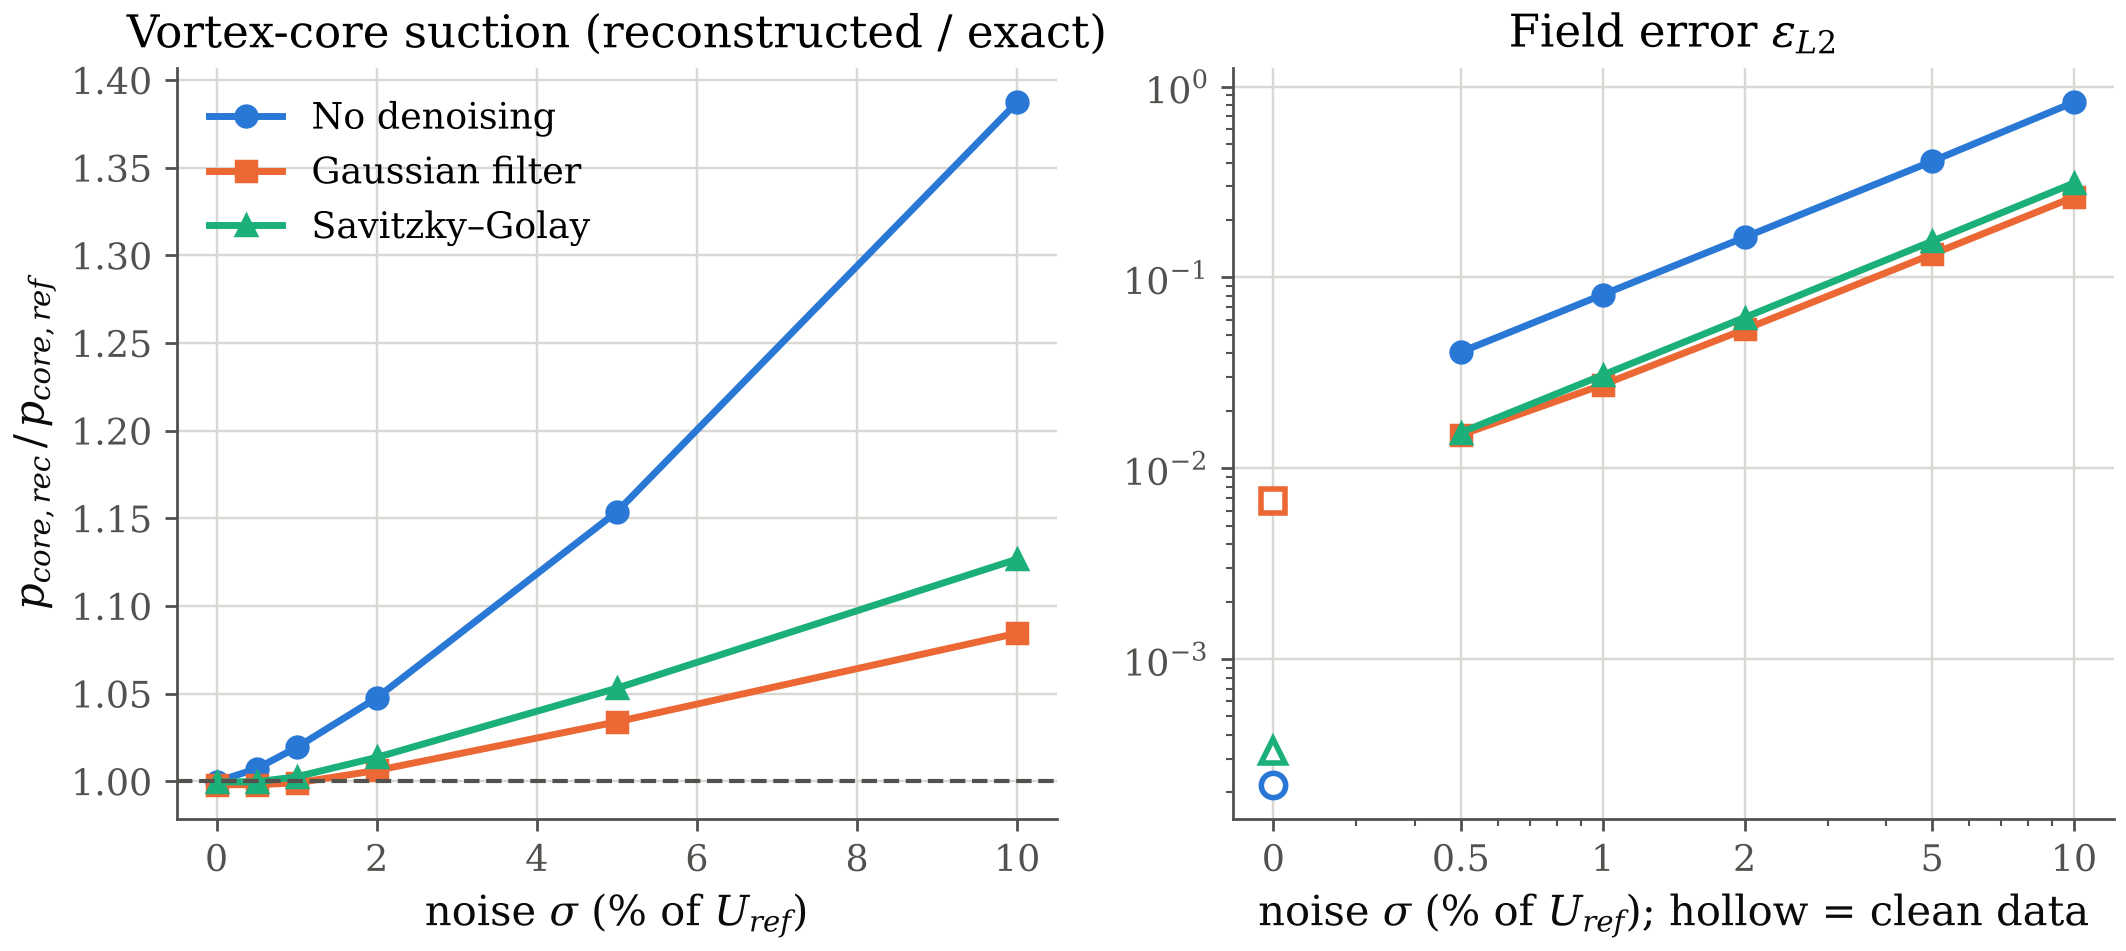
\includegraphics[width=0.85\linewidth]{img/f_denoise.png}
\caption{Taylor--Green core window. Left: reconstructed/exact vortex-core suction vs noise. Right: field error vs noise; hollow markers = clean data.}\end{figure}

\textbf{Window size $W$.} Averaging over the window smooths velocity. On the Taylor--Green core the suction drops only 0.3\,\% at $W=4h$, because the vortex (size $\sim\pi$) is much larger than the window ($4h\approx0.14$). On Kovasznay, with its sharp gradients near the inflow, $\eps_{L2}$ rises from 0.015 to 0.061 (clean). The effect grows with $W$ relative to the flow structure size, so it is expected to be much stronger for the cylinder-wake vortices.

\begin{table}[H]\centering\small
\begin{tabular}{@{}rccc@{}}\toprule
$\sigma$ (\%) & None & Gaussian & Savitzky--Golay\\\midrule
0 & 0.0002 & 0.0068 & 0.0003\\
0.5 & 0.041 & 0.015 & 0.015\\
1 & 0.081 & 0.027 & 0.031\\
2 & 0.162 & 0.053 & 0.062\\
5 & 0.406 & 0.132 & 0.155\\
10 & 0.828 & 0.264 & 0.312\\\bottomrule
\end{tabular}
\caption{Taylor--Green core window, $\eps_{L2}$ with and without denoising.}\end{table}

\begin{enumerate}
\item \textbf{Denoising cuts the noisy error about 3$\times$} at every noise level from 0.5\,\%.
\item \textbf{On clean data it hurts}: the Gaussian filter raises the error from 0.0002 to 0.007 because it also smooths the true signal. Savitzky--Golay barely changes clean data (it preserves quadratics), but on Kovasznay both filters help only above 0.5--1\,\%.
\item \textbf{Noise biases the core, not just scatters it.} Without denoising the core suction is \emph{over}-predicted, 1.39$\times$ at $\sigma=10\,\%$. The convective term multiplies noisy quantities, and products of zero-mean noise do not average to zero; also the minimum of a noisy field is biased low (a selection bias). Filtering reduces both.
\end{enumerate}

\begin{keyidea}[Smoothing trades noise for bias]
Window averaging, denoising and larger $\Delta t$ all reduce random error and add systematic error. The best setting depends on the noise level: none at $\sigma\approx0$, moderate above about 0.5\,\%.
\end{keyidea}

% ------------------------------------------------------------------
\chapter{Solver and convergence results}

\section{Residual histories}
\begin{figure}[H]\centering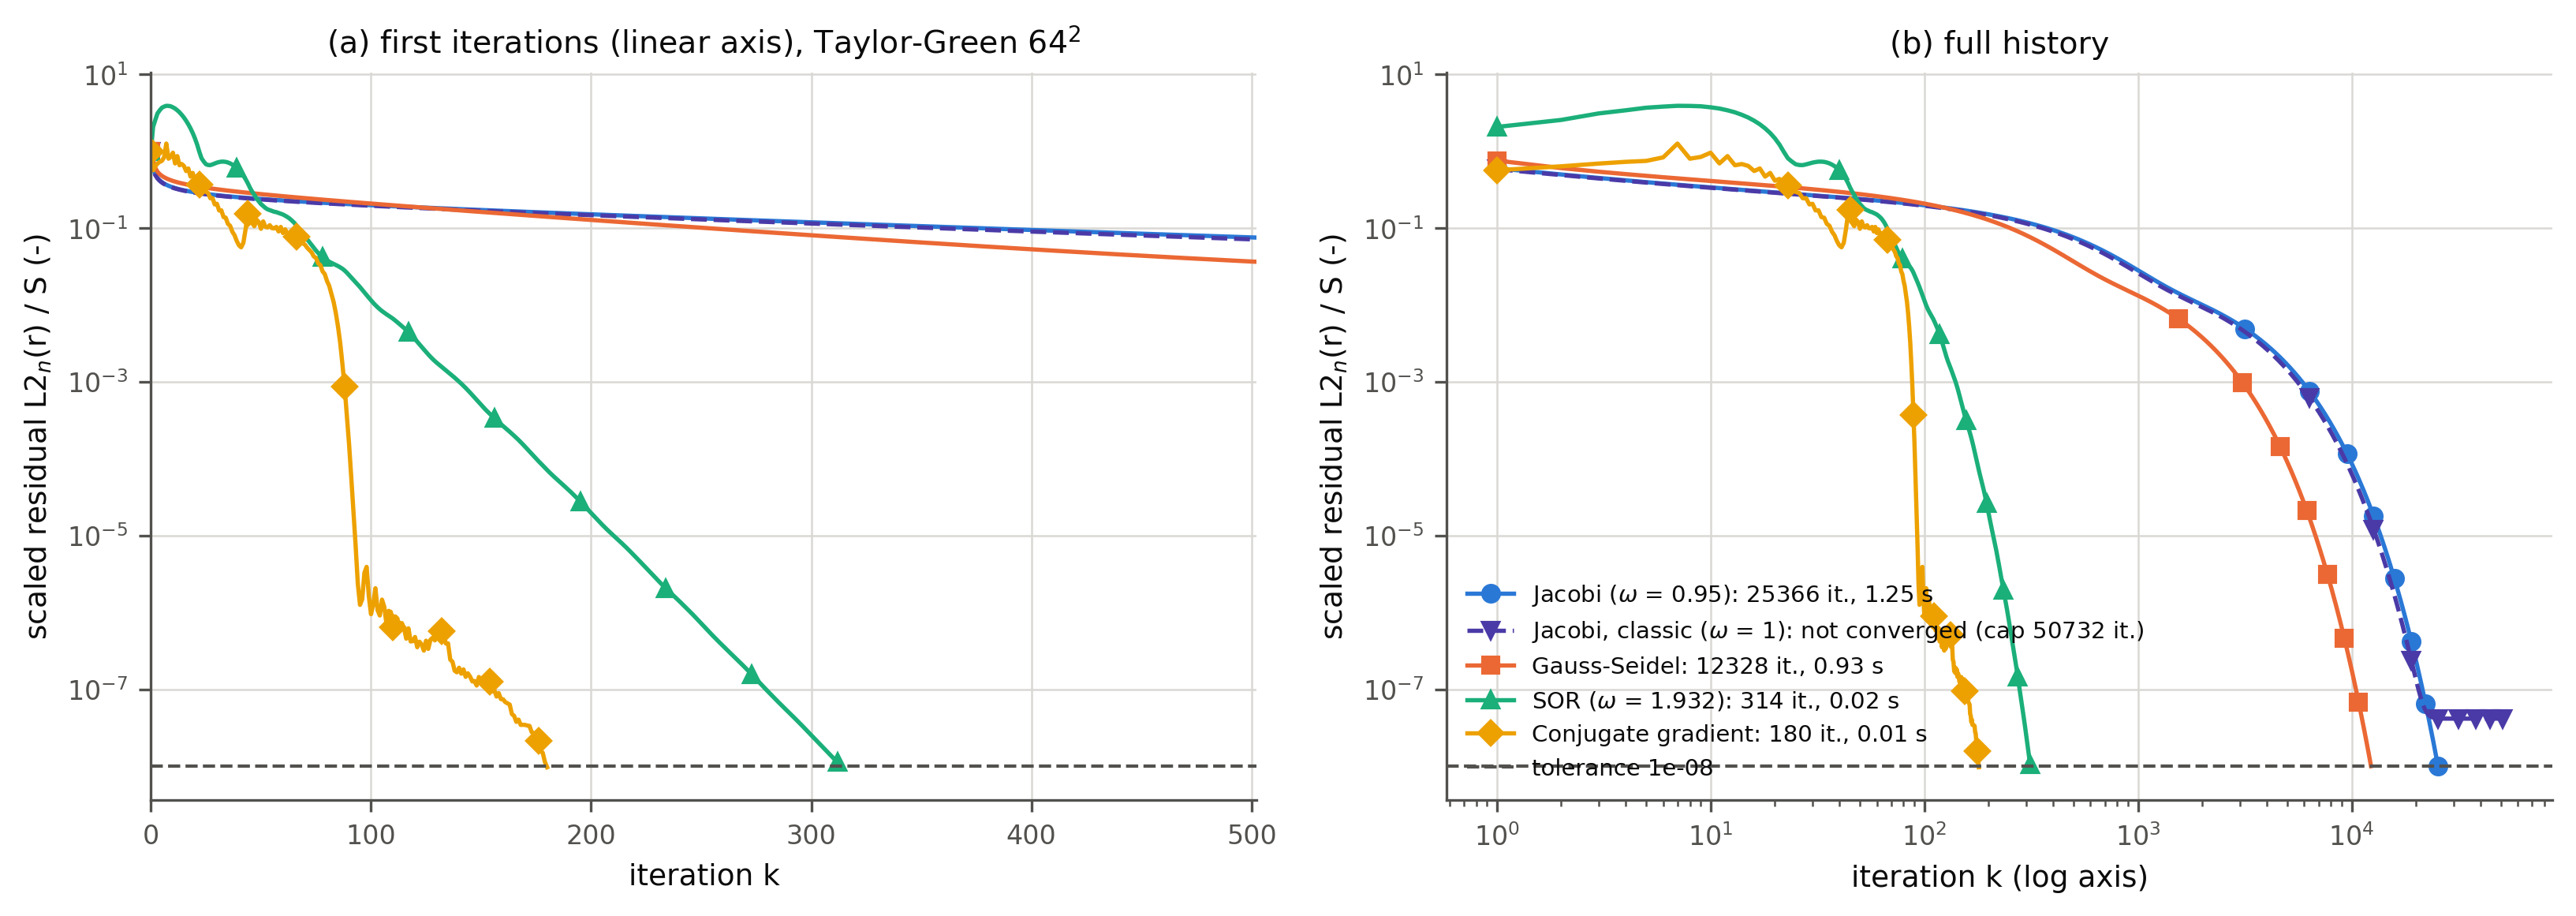
\includegraphics[width=\linewidth]{img/b_residuals.png}
\caption{Scaled residual history of five iterative solvers on the Taylor--Green $64^2$ Poisson system.}\end{figure}

\begin{table}[H]\centering\small
\begin{tabular}{@{}lrr@{}}\toprule
Solver ($64^2$, tol $10^{-8}$) & Iterations & Time\\\midrule
Jacobi ($\omega=0.95$) & 25\,366 & 1.3 s\\
Gauss--Seidel (red-black) & 12\,328 & 0.93 s\\
SOR ($\omega=1.932$) & 314 & 0.024 s\\
Conjugate gradient & 180 & 0.013 s\\
Jacobi, classic ($\omega=1$) & stalls at $4.2\times10^{-8}$ & --\\
Sparse direct (\code{spsolve}) & -- & $\approx$0.015 s\\\bottomrule
\end{tabular}\end{table}
Gauss--Seidel needs half the Jacobi iterations ($\rho_{GS}=\rho_J^2$); SOR and CG need 80--140$\times$ fewer. Classic Jacobi levels off above the tolerance: the checkerboard stall of Section~7.2. All solvers give the same pressure as the direct solve (agreement $<10^{-6}$).

\section{Iterations vs grid size and SOR stability}
\begin{figure}[H]\centering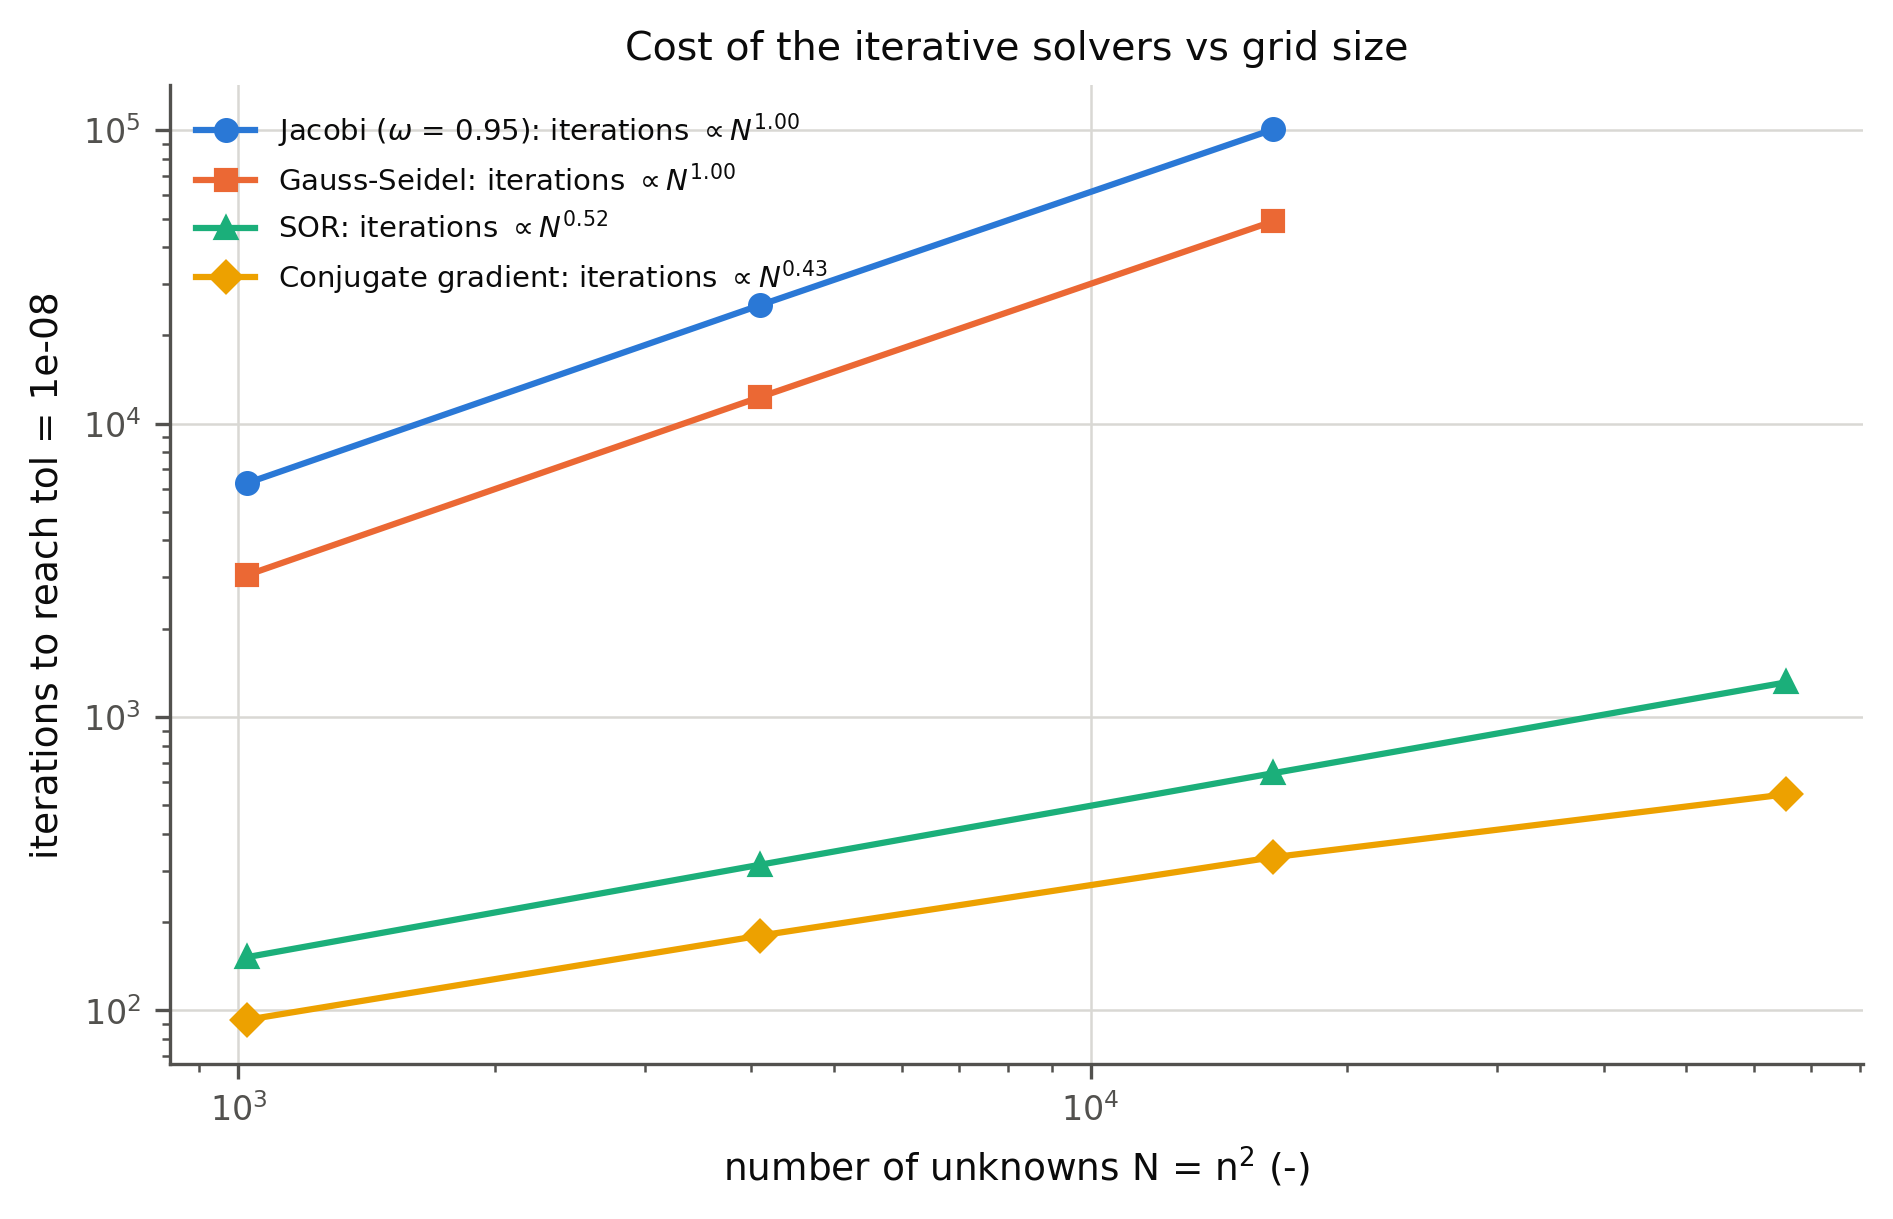
\includegraphics[width=0.7\linewidth]{img/fig14_iterations_vs_grid.png}
\caption{Iterations to converge vs number of unknowns $N$.}\end{figure}
Fitted exponents: Jacobi and Gauss--Seidel $N^{1.00}$, SOR $N^{0.52}$, CG $N^{0.43}$, as the theory predicts ($N$ for Jacobi/GS, $\sqrt N$ for optimal SOR and CG).

\begin{figure}[H]\centering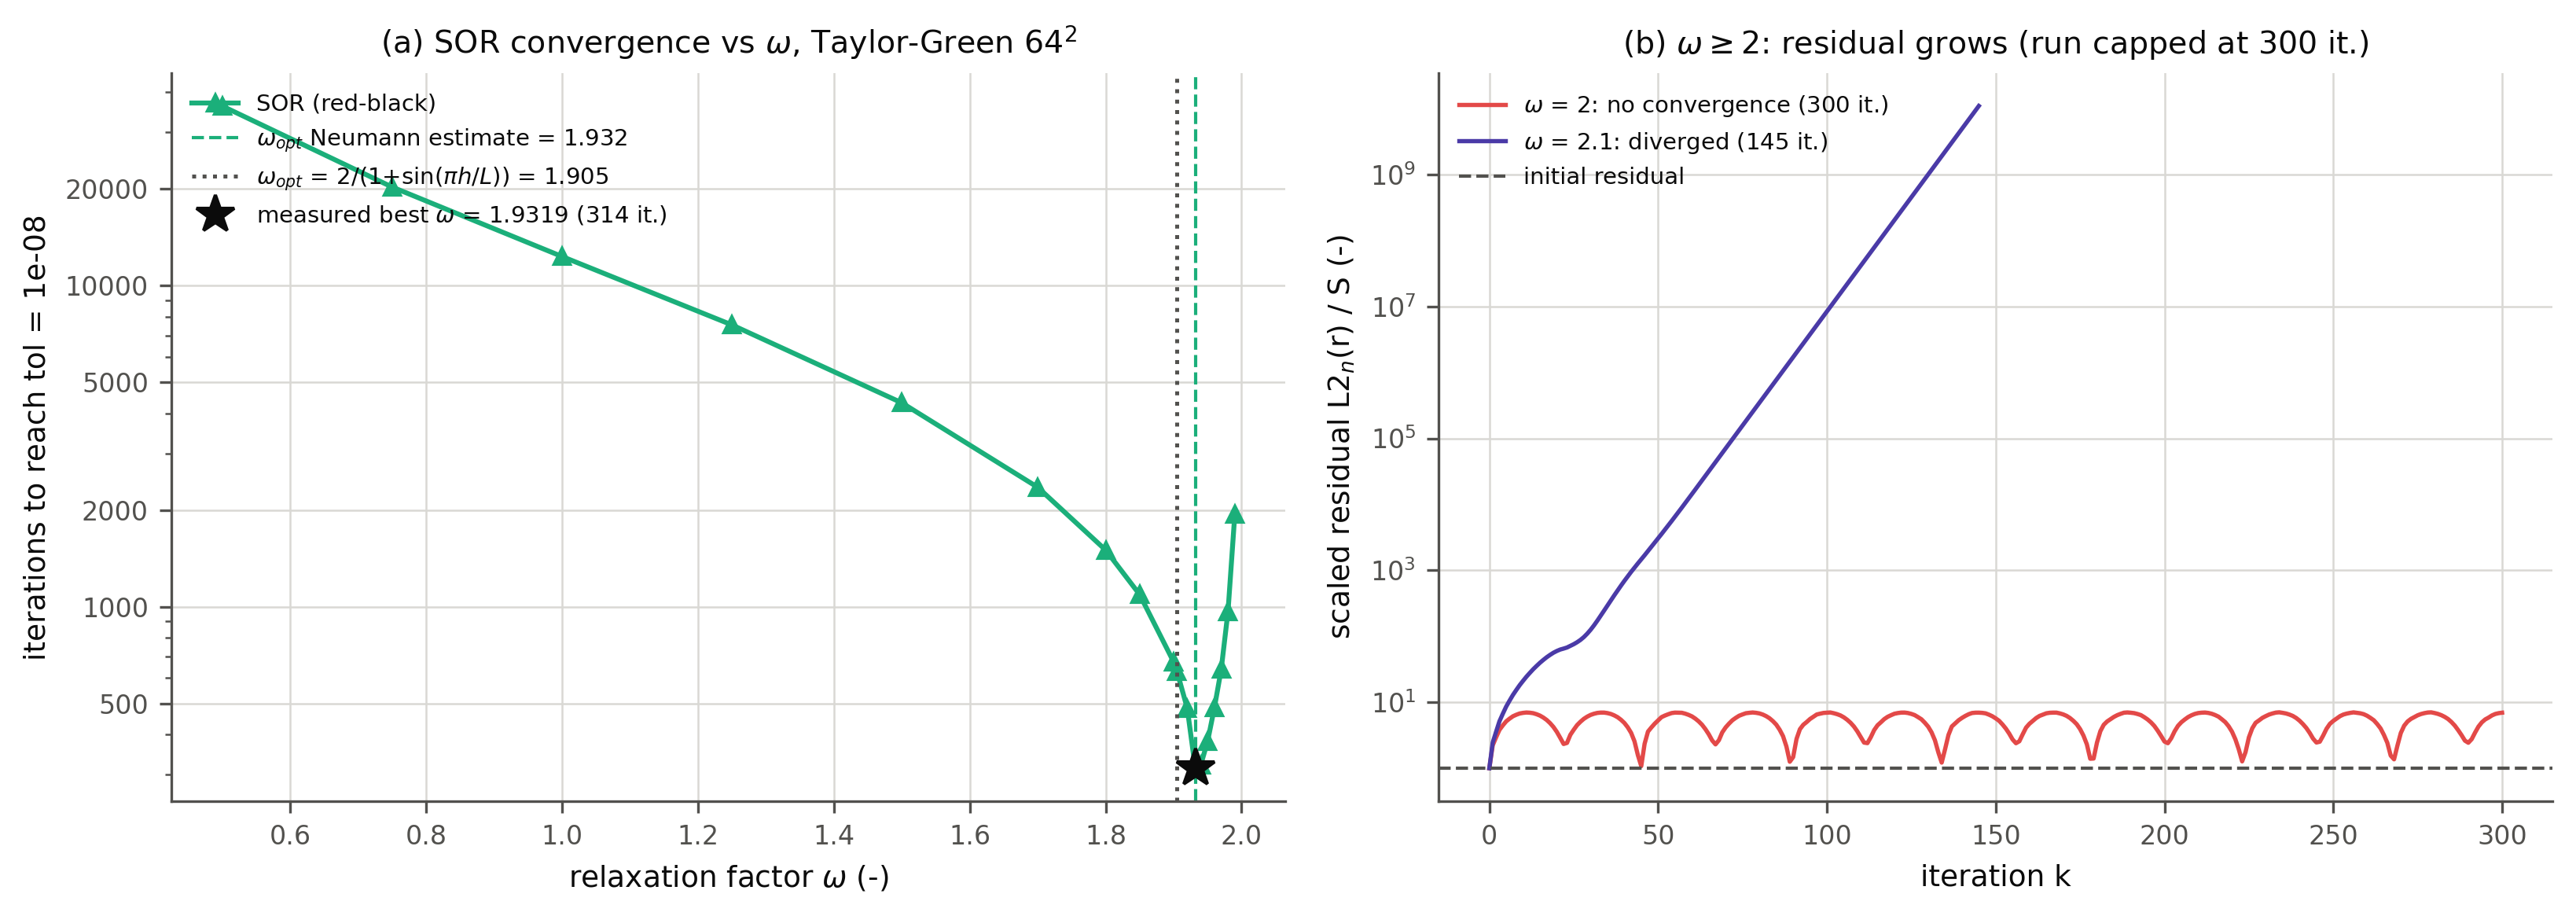
\includegraphics[width=\linewidth]{img/fig15_sor_stability.png}
\caption{(a) SOR iterations vs $\omega$; the measured optimum matches the Neumann estimate 1.932, not the Dirichlet formula 1.905. (b) $\omega=2$ does not converge and $\omega=2.1$ diverges (Kahan).}\end{figure}

\section{Residual vs change}
\begin{figure}[H]\centering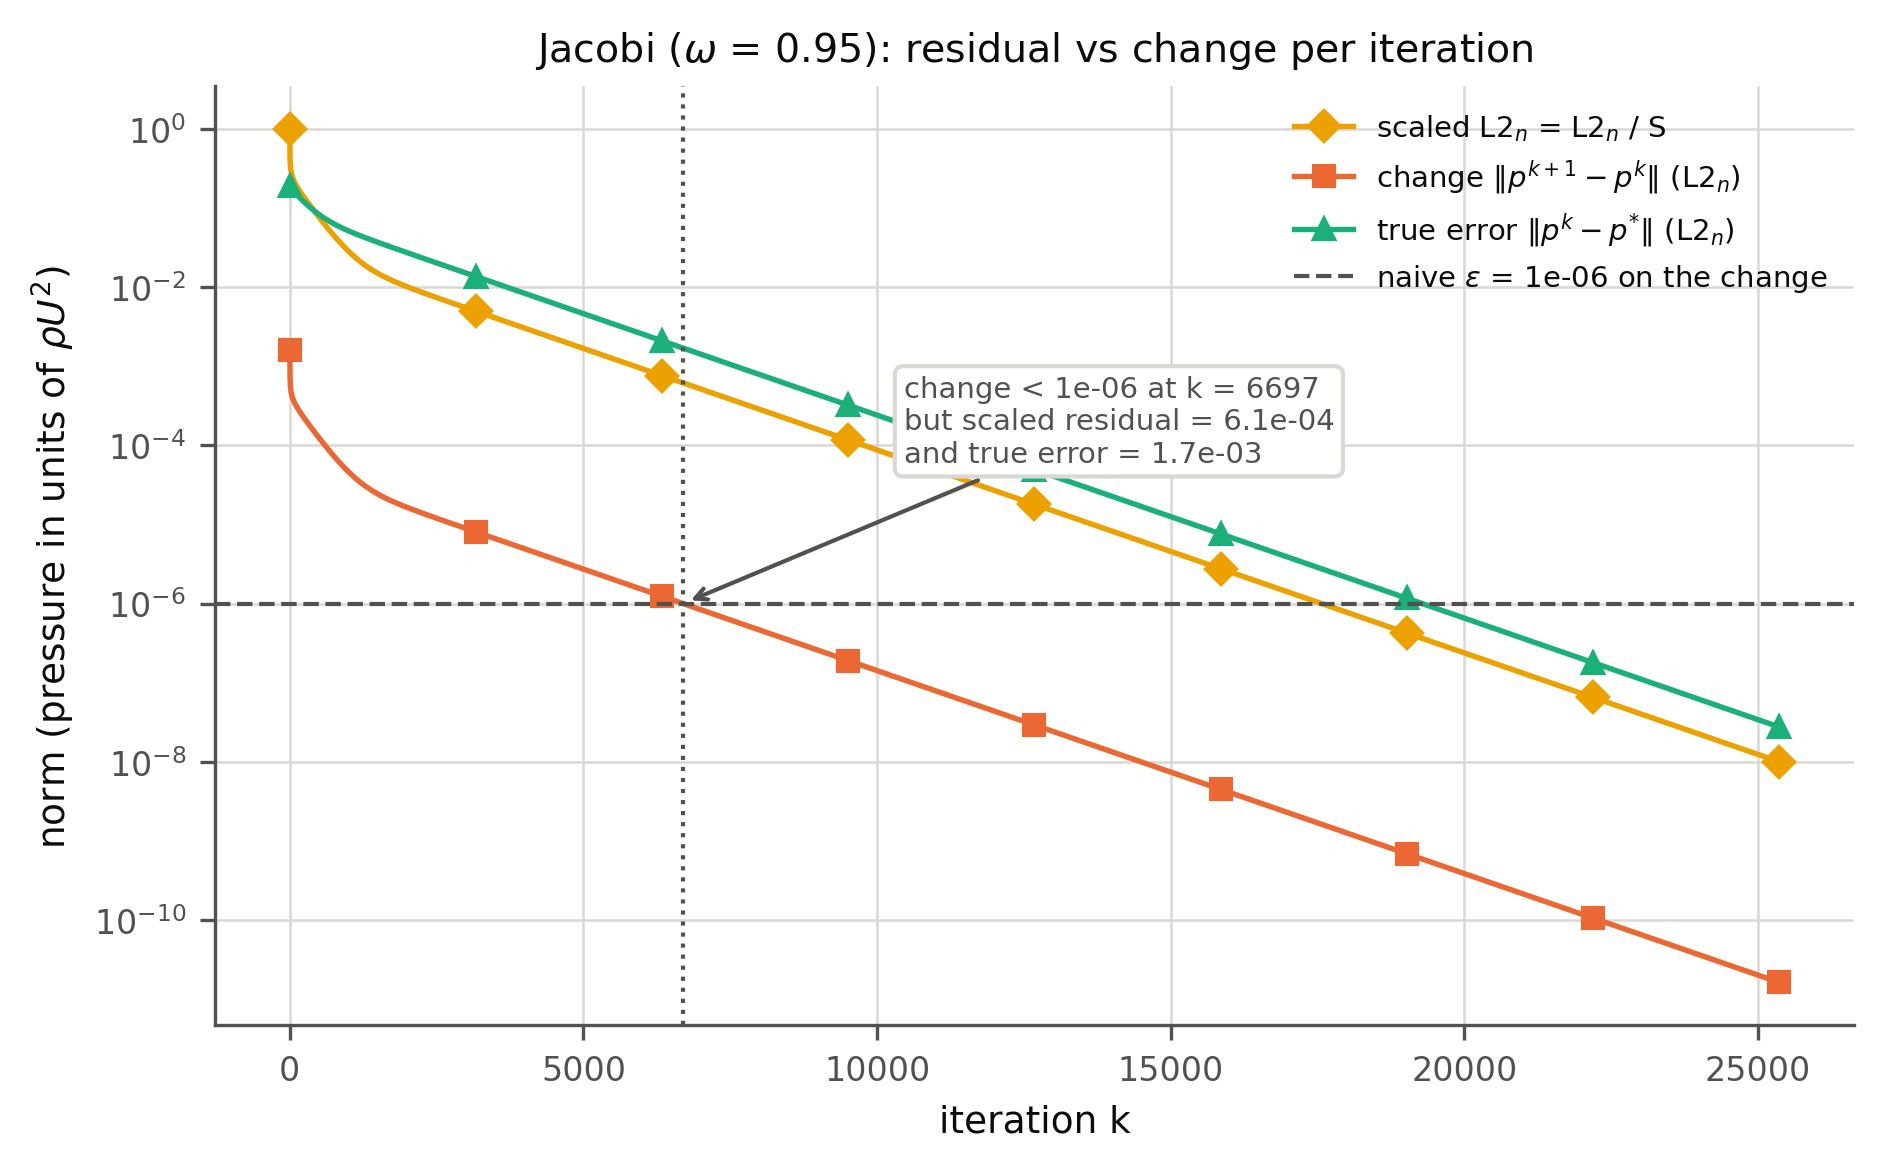
\includegraphics[width=0.72\linewidth]{img/fig13_residual_vs_change.png}
\caption{Jacobi: scaled residual, change per iteration and true error. When the change first drops below $10^{-6}$ the solution is still far from converged.}\end{figure}

\section{Norms across grids}
\begin{figure}[H]\centering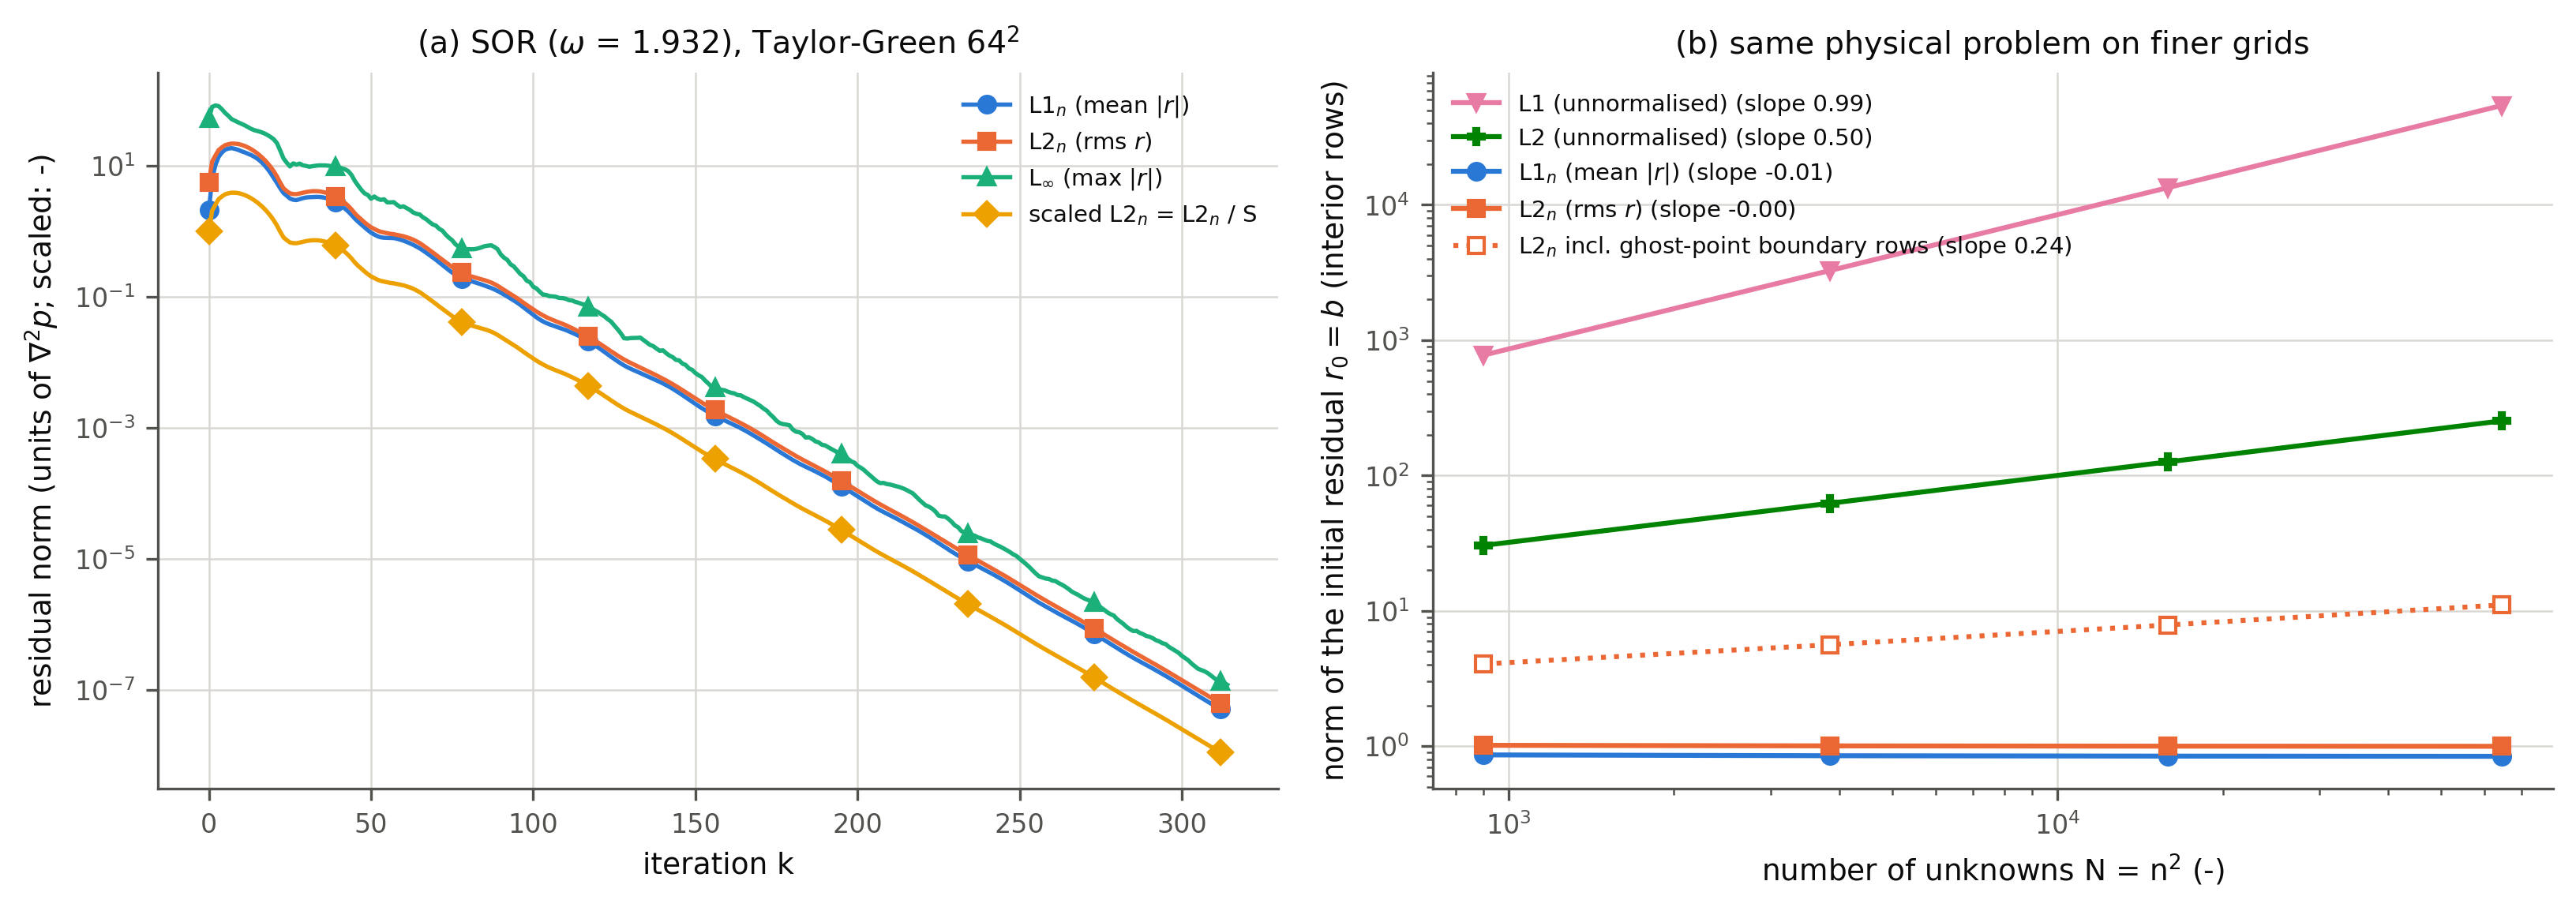
\includegraphics[width=\linewidth]{img/fig12_norm_comparison.png}
\caption{Different norms of the same residual. Unnormalised $L_1$, $L_2$ grow with grid size ($N^{0.99}$, $N^{0.50}$); normalised norms stay flat.}\end{figure}

\section{First- vs second-order schemes}
\begin{figure}[H]\centering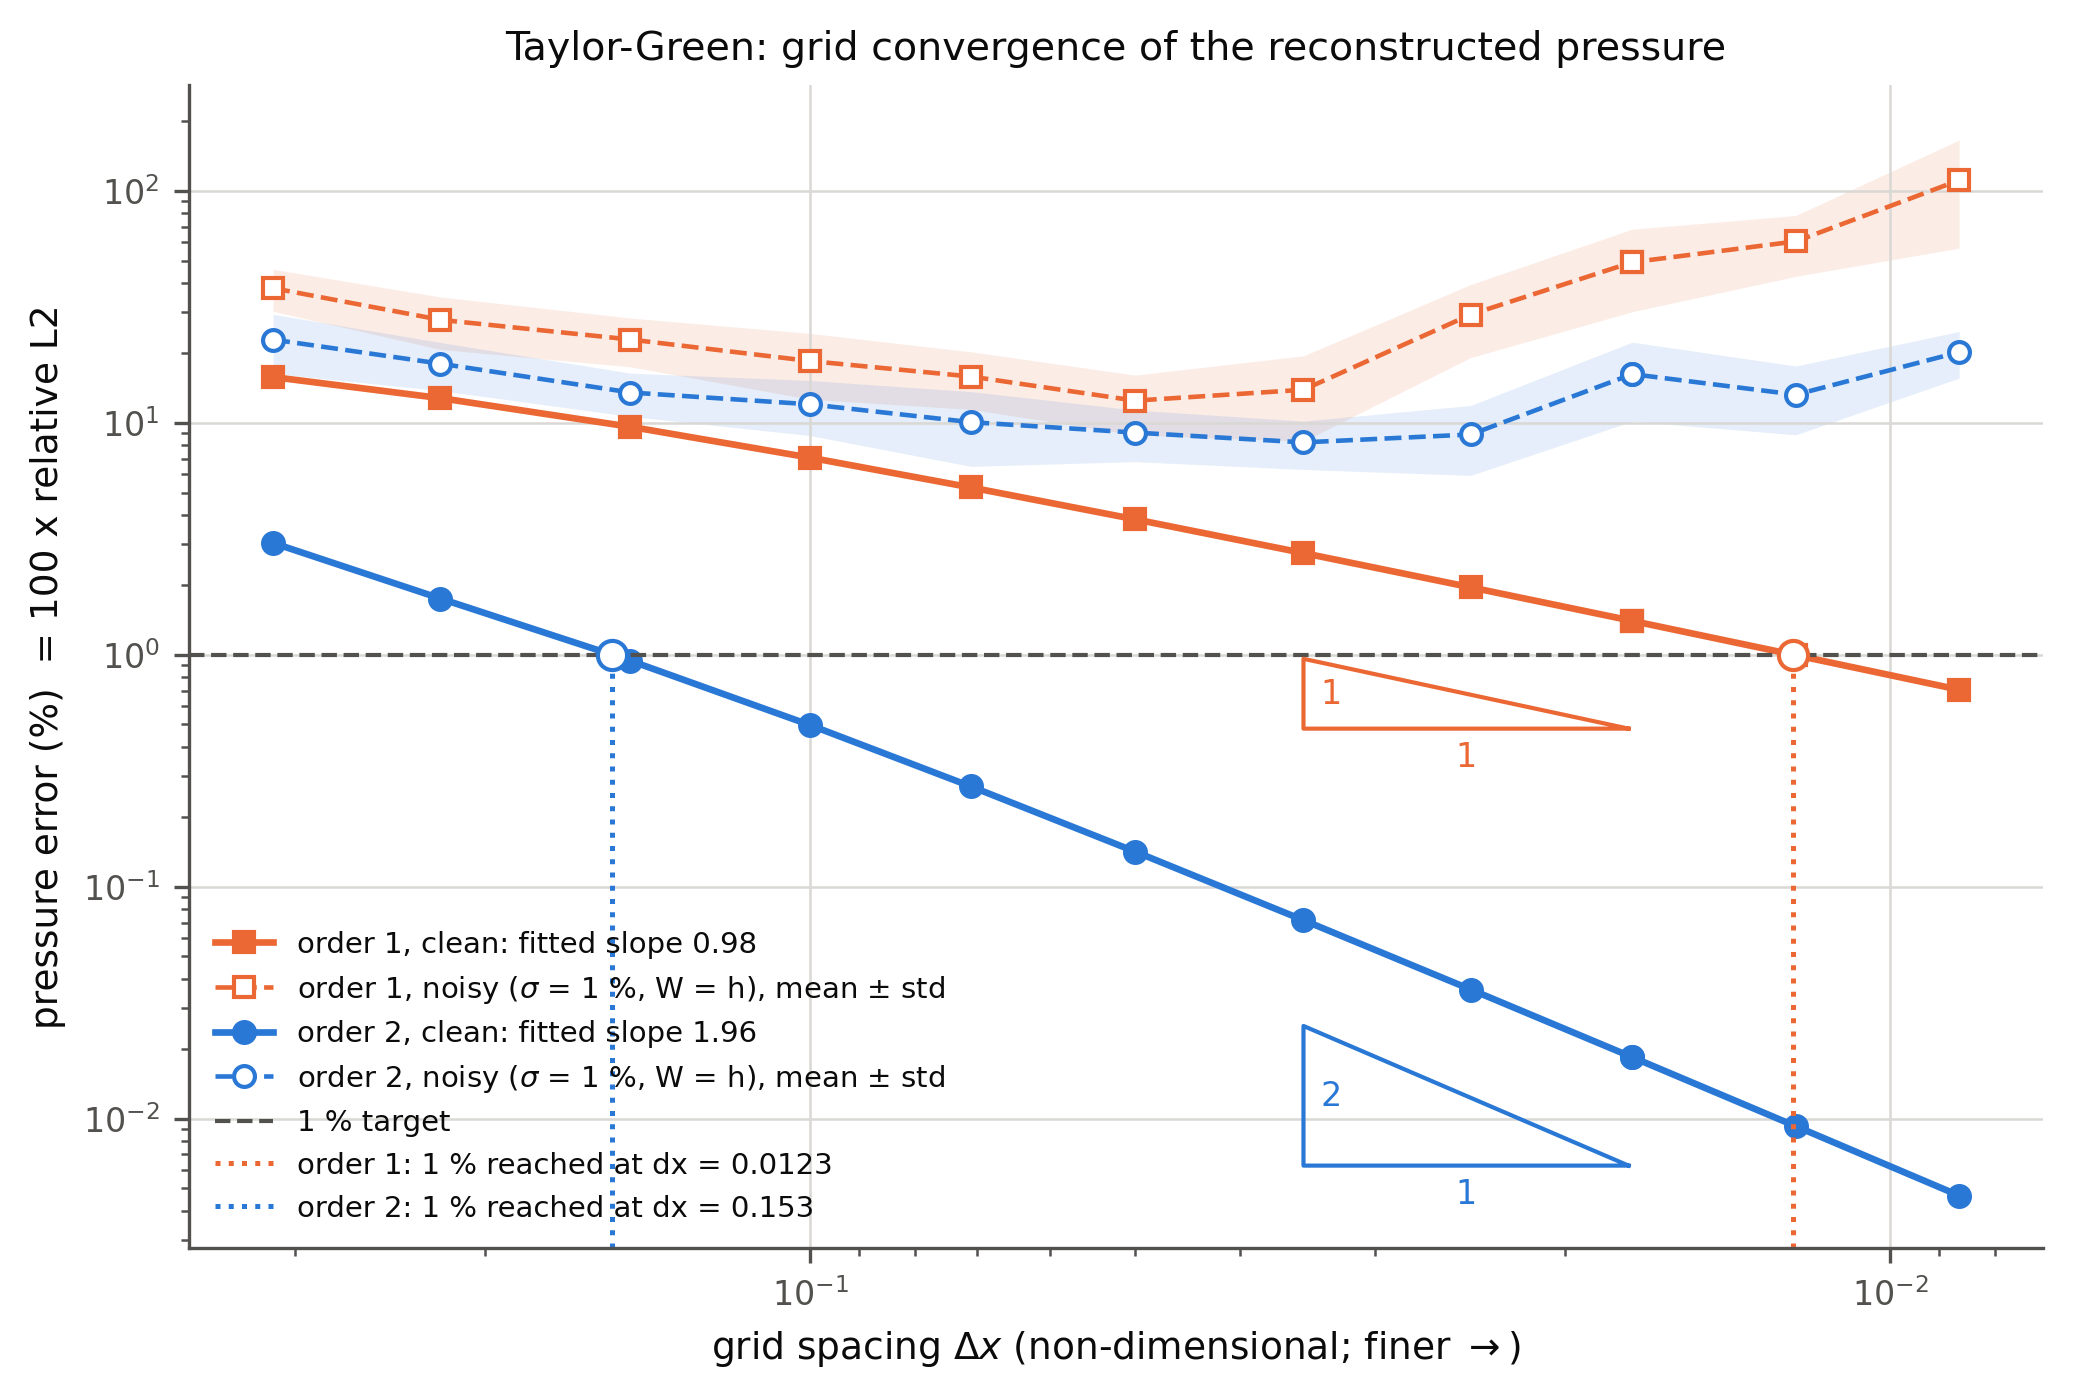
\includegraphics[width=0.72\linewidth]{img/b_order.png}
\caption{Grid convergence of the reconstructed pressure on Taylor--Green with first- and second-order stencils; dashed: 1\,\% noise.}\end{figure}

\begin{table}[H]\centering\small
\begin{tabular}{@{}lcccc@{}}\toprule
 & \multicolumn{2}{c}{Slope (finest 5 grids)} & \multicolumn{2}{c}{$\Delta x$ for 1\,\% error}\\
Case & order 1 & order 2 & order 1 & order 2\\\midrule
Taylor--Green & 0.98 & 1.96 & 0.0123 & 0.153\\
Kovasznay Re = 20 & 1.00 & 1.96 & 0.0033 (extrap.) & 0.026\\\bottomrule
\end{tabular}\end{table}
The second-order scheme reaches 1\,\% error on a grid about 12$\times$ coarser in each direction (Taylor--Green). To halve the error, order 1 must refine $\Delta x$ by 2, order 2 only by $\sqrt2$. With 1\,\% noise both curves level off and rise again; the second-order scheme stays lower.

\textbf{Why order 1 gives slope 1 even with an $O(1)$ boundary error.} The first-order Neumann row has an $O(1)$ local truncation error, but it acts only on a layer of width $O(h)$, so the global error is $O(h)$, the same argument that makes the second-order scheme's $O(h)$ boundary rows globally $O(h^2)$.

% ================================================================== PART V
\part{Simulation, literature and conclusions}

\chapter{The CFD case: a cylinder wake at Re = 100}
Exact solutions are smooth and simple. A real application is an unsteady wake with vortices shed from a body. The project therefore simulates the 2-D laminar flow past a circular cylinder at $Re=U_\infty D/\nu=100$ in OpenFOAM, samples it in a PIV-like window, and runs the same reconstruction on that data with the CFD pressure as the reference.

The three meshes were run with the OpenFOAM v2606 MinGW build on native Windows (4 cores, MS-MPI), and the solution was inspected in ParaView 6.2 (Figure~\ref{fig:paraview}).

\section{Why this flow}
\begin{itemize}
\item Above $Re\approx47$ the steady wake becomes unstable and vortices are shed alternately from the two sides: the \textbf{K\'arm\'an vortex street}. The flow is periodic with Strouhal number $St=fD/U\approx0.165$ at $Re=100$.
\item Below $Re\approx190$ the wake stays two-dimensional (Williamson 1996), so a 2-D simulation is physically valid and planar PIV would miss nothing.
\item The shed vortices are \emph{convected} at nearly the free-stream speed while they spin more slowly: exactly the $w<c$ situation where the Lagrangian material derivative should win.
\end{itemize}

\section{Domain, mesh and boundary conditions}
\begin{figure}[H]\centering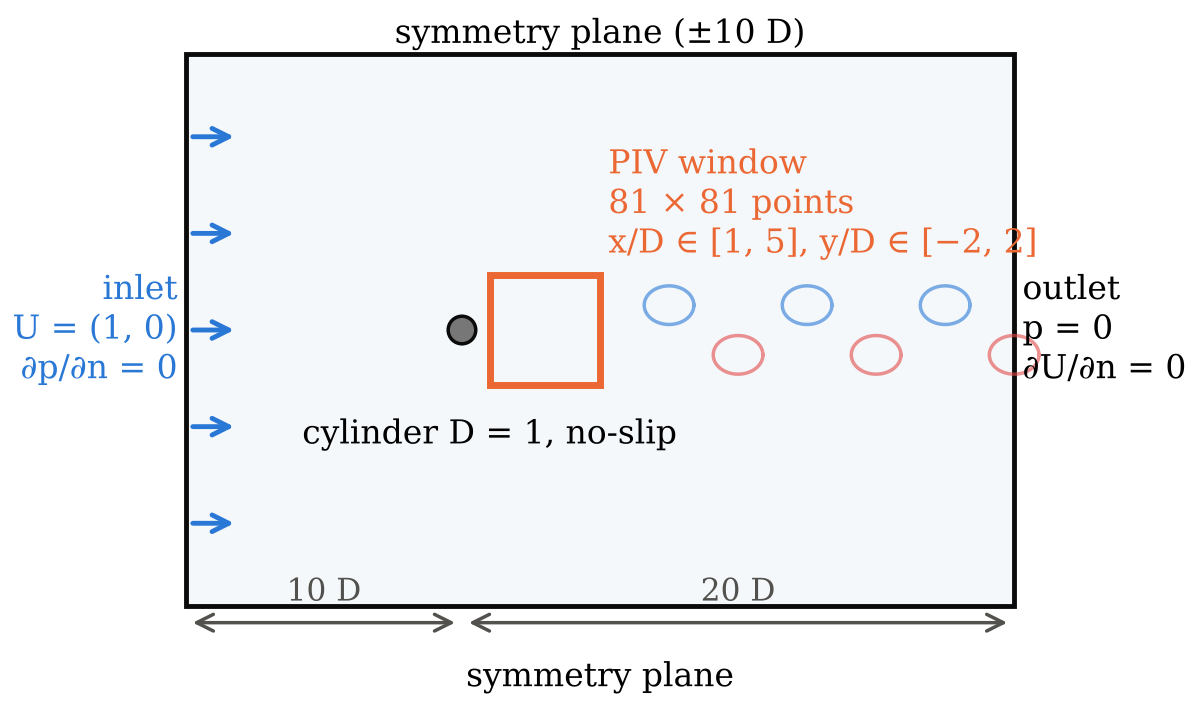
\includegraphics[width=0.62\linewidth]{img/f_cfd_domain.png}
\caption{Computational domain (not to scale), boundary conditions and the PIV sampling window.}\end{figure}

\begin{itemize}
\item \textbf{Non-dimensional set-up:} $D=1$, $U_\infty=1$, $\nu=0.01$, $\rho=1$.
\item \textbf{Domain:} 10\,$D$ upstream, 20\,$D$ downstream, $\pm10\,D$ laterally; one cell thick in $z$ with \code{empty} front and back patches (OpenFOAM's way of making a case 2-D).
\item \textbf{Boundary conditions:}
\begin{itemize}
\item inlet: $\uu=(1,0)$, $\partial p/\partial n=0$;
\item outlet: $\partial\uu/\partial n=0$, $p=0$;
\item sides: \code{symmetryPlane} (zero normal velocity and zero shear);
\item cylinder: no-slip.
\end{itemize}
\item \textbf{Blockage:} the side walls are 20\,$D$ apart, so the blockage is $D/H=5\,\%$. It slightly accelerates the flow past the cylinder and raises $C_D$ and $St$ above unbounded-domain values.
\item \textbf{Mesh:} an O-grid around the cylinder (body-fitted, near-orthogonal cells clustered radially at the wall for the boundary layer) out to the square $[-2,2]^2$, plus 8 rectangular blocks. Generated with \code{blockMesh} from a dictionary written by \code{cfd/generate\_cases.py}, which also checks the block topology.
\end{itemize}

\begin{table}[H]\centering\small
\begin{tabular}{@{}lrccc@{}}\toprule
Mesh & Cells & Cylinder tangential cell & First radial cell & Wake $\Delta y$\\\midrule
Coarse & 6\,690 & 0.033 & 0.022 & 0.167\\
Medium & 26\,760 & 0.016 & 0.011 & 0.083\\
Fine & 107\,040 & 0.008 & 0.0055 & 0.042\\\bottomrule
\end{tabular}
\caption{The three meshes: each level halves the cell size in both directions (4$\times$ the cells).}\end{table}

\section{Solver and numerics}
\begin{itemize}
\item \textbf{Solver:} \code{pimpleFoam}, laminar, run in PISO mode (\code{nOuterCorrectors 1}, \code{nCorrectors 2}, one non-orthogonal corrector).
\item \textbf{Time scheme:} \code{backward} (second-order implicit). \textbf{Convection:} \code{linearUpwind} (second-order upwind-biased).
\item \textbf{Time step:} adaptive, keeping the maximum Courant number $Co=|u|\Delta t/\Delta x\le0.5$ (with $\Delta t\le0.01$); the run goes to $t=200$, about 33 shedding periods.
\item \textbf{Start-up kick:} a perfectly symmetric mesh and inflow can delay shedding for a long time. The inlet carries $v=0.1$ for $t<5$, ramped to 0 at $t=6$; from $t=6$ on it is exactly $\uu=(1,0)$.
\end{itemize}

\textbf{How PISO works, and why it connects to this project.} In incompressible flow there is no equation \emph{for} pressure; pressure is whatever makes the velocity divergence-free. Each time step, PISO:
\begin{enumerate}
\item solves the momentum equation with the old pressure (a predicted velocity that is not divergence-free);
\item takes the divergence of the momentum equation to get a \textbf{pressure Poisson equation}, $\nabla\cdot(\tfrac1a\nabla p)=\nabla\cdot\mathbf H$, and solves it;
\item corrects the velocity and fluxes with the new pressure gradient, and repeats steps 2--3 (here two pressure correctors per step, \code{nCorrectors 2}; the pressure equation is solved with the GAMG multigrid solver).
\end{enumerate}
So the CFD solver itself recovers pressure from velocity through a Poisson equation every time step, the same mathematical step the reconstruction performs on measured data. The difference: the CFD solver has exact boundary conditions and noise-free velocity; PIV has neither.

\section{Outputs and how they are processed}
\begin{itemize}
\item \textbf{Forces:} the \code{forceCoeffs} function object writes $C_D(t)$ and $C_L(t)$ every step.
\item \textbf{PIV window:} on the fine mesh, a run-time \code{sets} function object samples $\uu$ and $p$ on an $81\times81$ grid, $x/D\in[1,5]$, $y/D\in[-2,2]$, every 0.05 time units for $t\in[175,200]$ (about 4 shedding periods). Sampling at run time avoids writing about 500 full-field dumps.
\item \code{cfd/export\_window.py} converts the samples into one array file, which the studies load as a \code{FlowField}.
\end{itemize}

\subsection{Strouhal number, drag and lift}
$C_L(t)$ is resampled on a uniform time grid (the time step is adaptive), multiplied by a Hann window (to limit spectral leakage from a non-integer number of periods), zero-padded and Fourier transformed. The peak frequency, refined by parabolic interpolation, gives $St=fD/U_\infty$. Mean $C_D$ and the $C_L$ amplitude $(\max-\min)/2$ are taken over the last 80 time units.

\subsection{Is the wake fully developed? Periodicity, not steady state}
A periodic flow never satisfies a steady-state criterion $\|\uu^{n+1}-\uu^n\|<\eps$, and its solver residuals level off instead of falling to zero (each step starts from a changed flow). The project instead cuts $C_L(t)$ into cycles at upward zero crossings and declares the flow periodic once the cycle-to-cycle changes of amplitude and period both stay below $10^{-3}$ for three consecutive cycles.

\subsection{Grid independence: Richardson extrapolation and GCI}
For a quantity $f$ (St, $\bar C_D$) on fine, medium and coarse meshes ($f_1,f_2,f_3$) with representative cell sizes $h=\sqrt{\text{area}/\text{cells}}$ and ratios $r_{21}=h_2/h_1$, $r_{32}=h_3/h_2$ (Celik et al.\ 2008):
\begin{align}
e_{21}&=f_2-f_1,\quad e_{32}=f_3-f_2,\\
p&=\frac{\big|\ln|e_{32}/e_{21}|+\ln\frac{r_{21}^p-s}{r_{32}^p-s}\big|}{\ln r_{21}},\quad s=\operatorname{sign}(e_{32}/e_{21})\quad\text{(solved by fixed-point iteration)},\\
f_{ext}&=\frac{r_{21}^pf_1-f_2}{r_{21}^p-1},\qquad
GCI_{fine}=\frac{1.25\,|e_{21}/f_1|}{r_{21}^p-1}.
\end{align}
$p$ is the observed order of accuracy (expected 1--2), $f_{ext}$ the extrapolated grid-converged value, and GCI a conservative error band on the fine-mesh value (safety factor 1.25 for three-grid studies). The asymptotic ratio $GCI_{medium}/(r_{21}^pGCI_{fine})\approx1$ confirms the meshes are in the asymptotic range.

\section{Results}

\subsection{The flow field}
\begin{figure}[H]\centering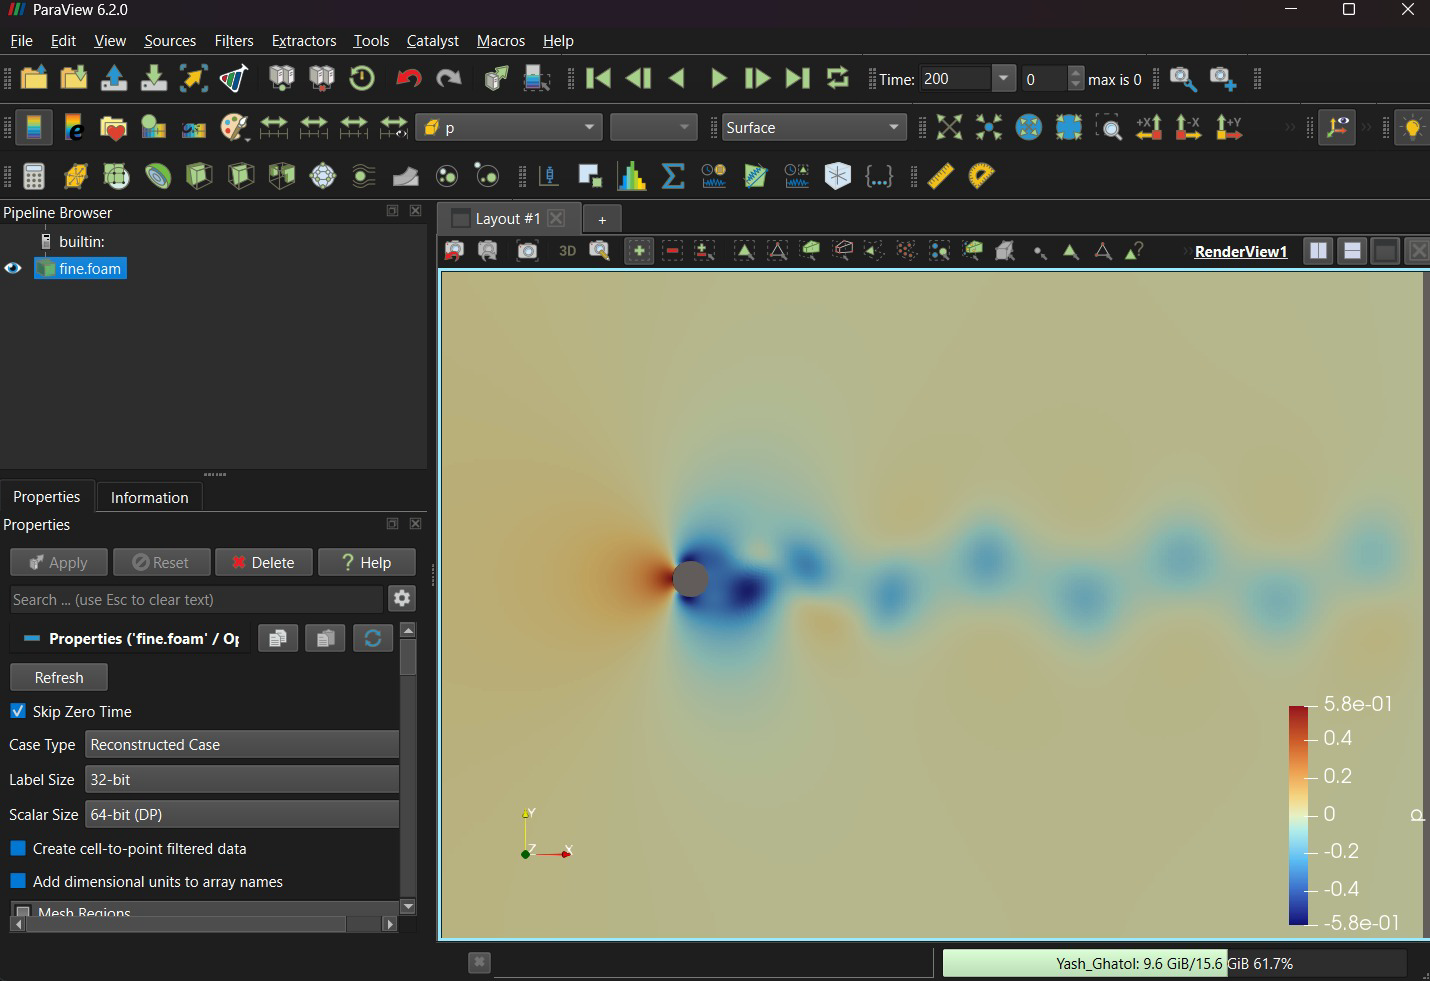
\includegraphics[width=0.9\linewidth]{img/c_paraview.png}
\caption{ParaView 6.2 screenshot (unedited) of the fine-mesh OpenFOAM solution at $t=200$, coloured by pressure. High pressure (red) at the front stagnation point, low pressure on the sides, and a K\'arm\'an street of low-pressure vortex cores alternating above and below the centreline.}\label{fig:paraview}\end{figure}

\subsection{Grid independence}
\begin{table}[H]\centering\small
\begin{tabular}{@{}lrccc@{}}\toprule
Mesh & Cells & $St$ & $\bar C_D$ & $C_L$ amplitude\\\midrule
Coarse & 6\,690 & 0.1644 & 1.3754 & 0.3216\\
Medium & 26\,760 & 0.1688 & 1.3880 & 0.3451\\
\textbf{Fine} & \textbf{107\,040} & \textbf{0.1695} & \textbf{1.3879} & \textbf{0.3451}\\
Richardson extrapolation & -- & 0.1697 & converged & converged\\\midrule
2-D simulations, Re = 100 (approx.) & -- & 0.164--0.165 & $\approx1.33$ & $\approx0.33$\\\bottomrule
\end{tabular}
\caption{Grid independence (analysis window: last 80 time units, 13--14 shedding periods per mesh; amplitude drift $\le0.04\,\%$).}\end{table}

\begin{table}[H]\centering\footnotesize\setlength{\tabcolsep}{4pt}
\begin{tabular}{@{}lccccccc@{}}\toprule
Quantity & coarse$\to$medium & medium$\to$fine & $p$ & $f_{ext}$ & GCI$_{medium}$ & GCI$_{fine}$ & asympt.\ ratio\\\midrule
$St$ & 2.67\,\% & 0.46\,\% & 2.48 & 0.1697 & 0.71\,\% & 0.13\,\% & 1.005\\
$\bar C_D$ & 0.91\,\% & 0.00\,\% & -- & -- & -- & -- & --\\
$C_L$ amplitude & 7.30\,\% & 0.01\,\% & -- & -- & -- & -- & --\\\bottomrule
\end{tabular}
\caption{Richardson extrapolation and grid convergence index, from \code{grid\_independence.md}.}\end{table}

\begin{figure}[H]\centering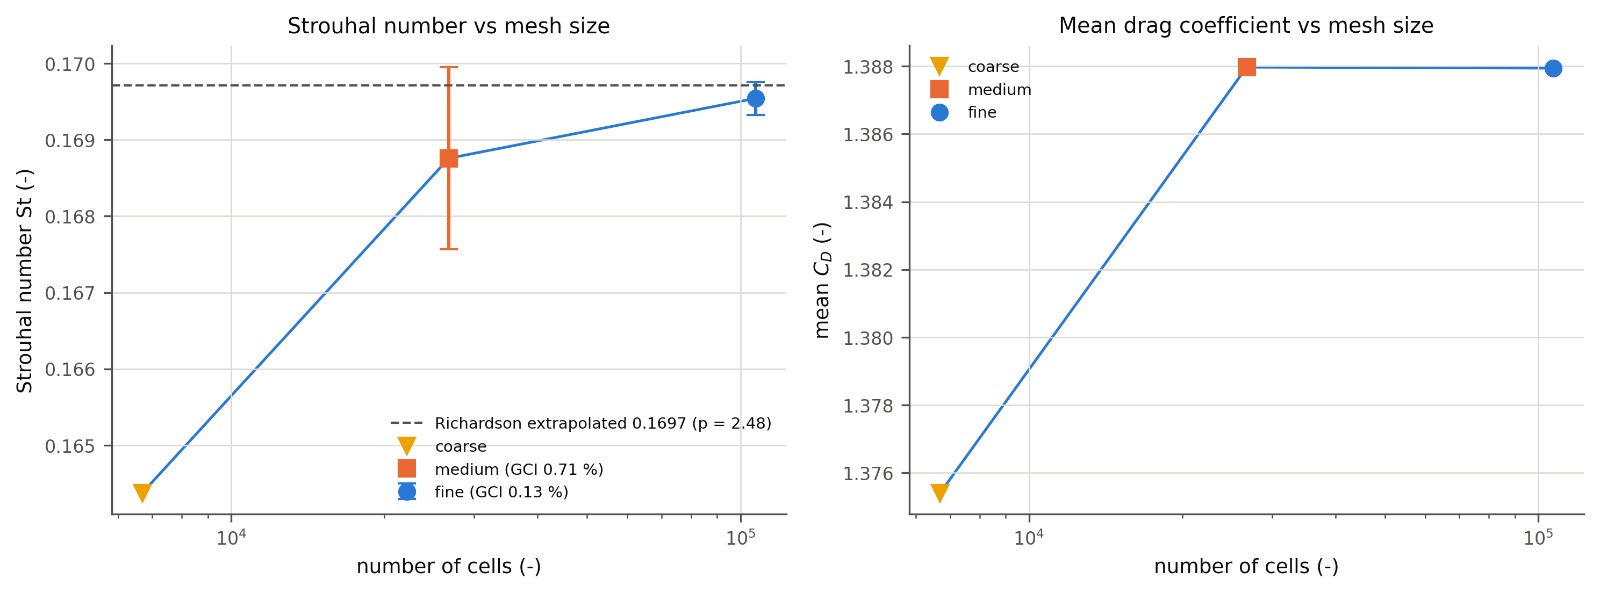
\includegraphics[width=\linewidth]{img/c_st.png}
\caption{Strouhal number and mean drag vs number of cells; error bars on St are the GCI; dashed line the Richardson-extrapolated value.}\end{figure}

\begin{itemize}
\item \textbf{St converges monotonically}: the change falls from 2.67\,\% to 0.46\,\% per refinement. The observed order $p=2.48$ is close to the nominal second order of the schemes, the extrapolated value is 0.1697 and the fine-mesh GCI is 0.13\,\%. The asymptotic ratio 1.005 ($\approx1$) shows the three meshes are in the asymptotic range.
\item \textbf{Mean drag and lift amplitude converge already on the medium mesh} (changes 0.00\,\% and 0.01\,\%). With $e_{21}\approx0$ the observed order is undefined (the ratio $e_{32}/e_{21}$ blows up), so no Richardson value is reported: the medium--fine difference is below the resolution of the time averaging.
\item The \textbf{coarse mesh} under-predicts both St and the lift amplitude (0.322 vs 0.345): with a 0.022\,$D$ first cell it under-resolves the boundary layer and the separation.
\end{itemize}

\begin{figure}[H]\centering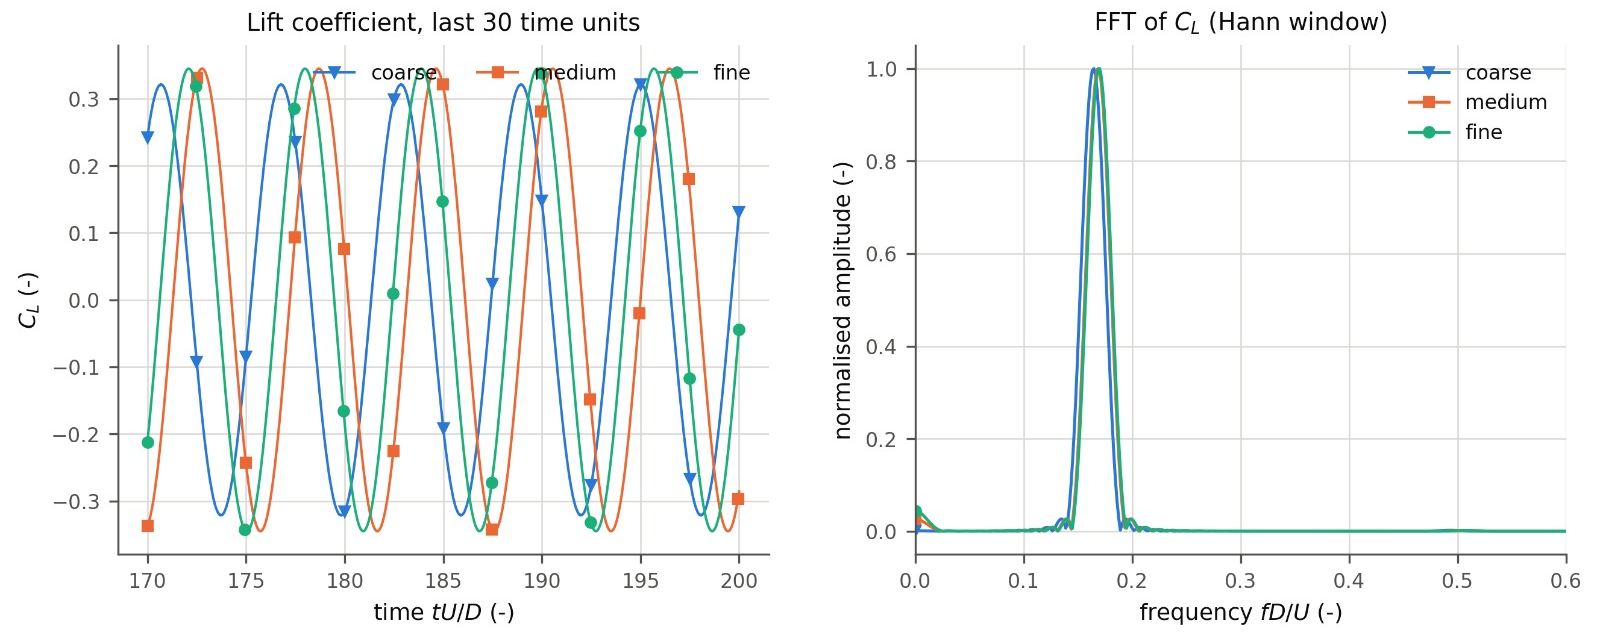
\includegraphics[width=\linewidth]{img/c_clfft.png}
\caption{Lift coefficient over the last 30 time units for the three meshes, and its spectrum (Hann window). The single sharp peak at $fD/U\approx0.17$ is the shedding frequency.}\end{figure}

\subsection{Residuals and periodicity}
\begin{figure}[H]\centering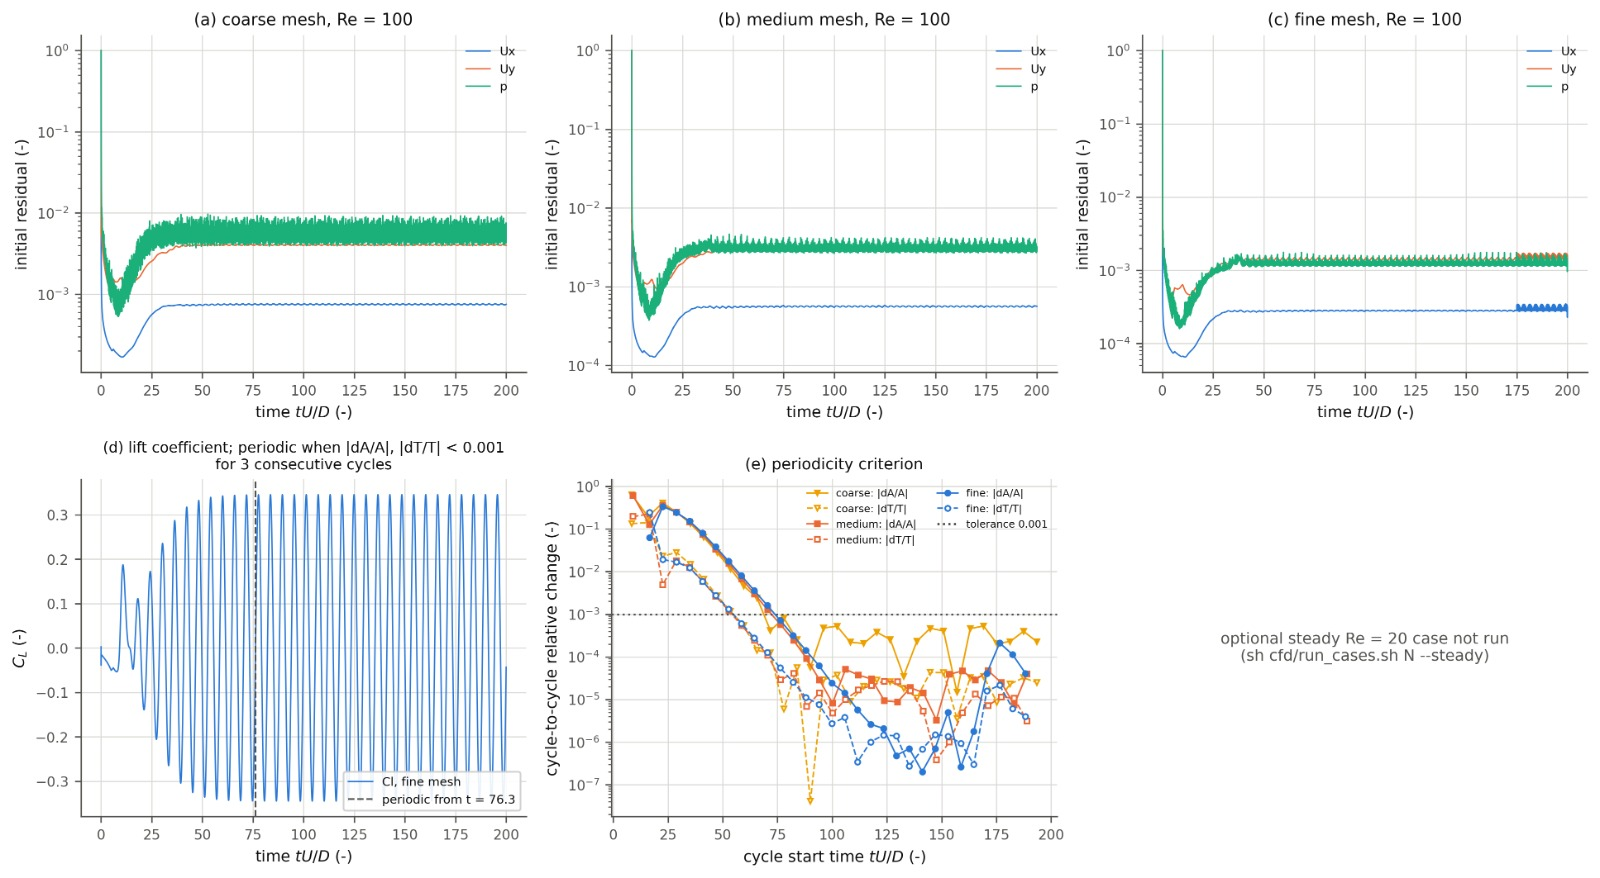
\includegraphics[width=\linewidth]{img/c_resid.png}
\caption{(a)--(c) Initial residuals of $U_x$, $U_y$ and $p$ for the three meshes; (d) fine-mesh lift, periodic from $t=76.3$; (e) cycle-to-cycle relative change of the lift amplitude and period.}\end{figure}
\begin{itemize}
\item \textbf{Residuals level off} (fine mesh: about $10^{-3}$ for $p$ and $U_y$, $3\times10^{-4}$ for $U_x$) instead of falling to zero. This is expected for a periodic flow: every time step starts from a changed flow (Section~12.4.2). Finer meshes level off lower. The small step on the fine mesh after $t=175$ coincides with the start of window sampling, which also caps the time step to hit the sample times.
\item \textbf{The wake is periodic from $t=76.3$} on the fine mesh: the cycle-to-cycle change of amplitude and period stays below $10^{-3}$. The PIV window ($t=175$--200) is therefore fully developed. The coarse mesh hovers around the tolerance, another sign of under-resolution.
\end{itemize}

\subsection{Pressure reconstructed from the CFD velocity}
\begin{figure}[H]\centering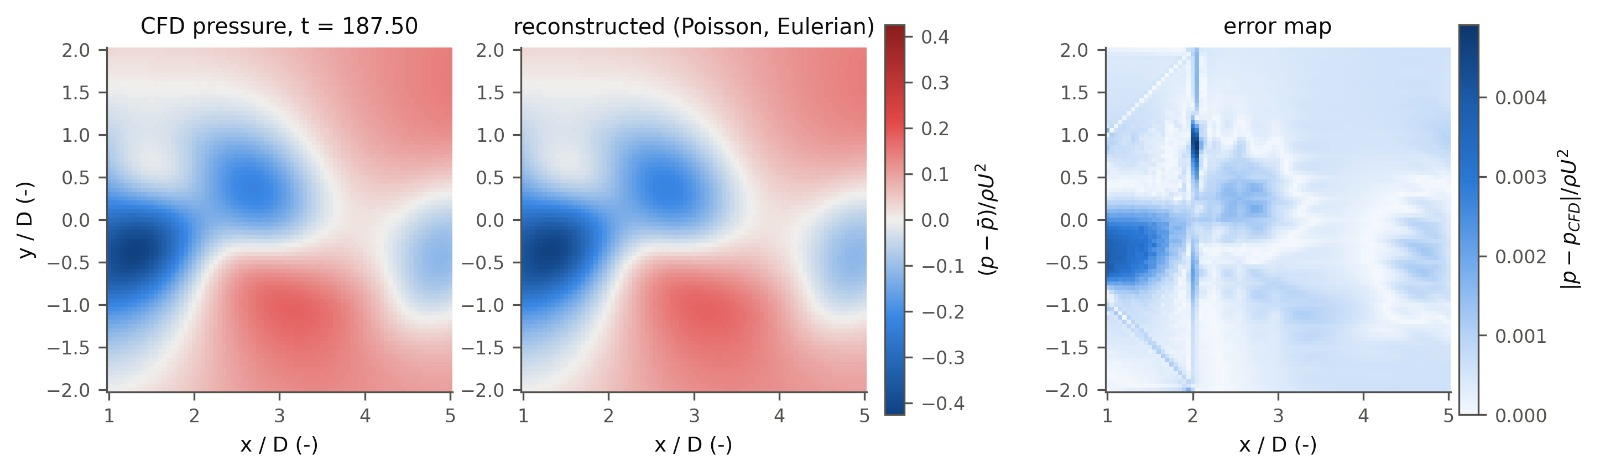
\includegraphics[width=\linewidth]{img/c_fields.png}
\caption{At $t=187.5$: CFD pressure in the window, pressure reconstructed from the CFD velocity samples (Poisson, Eulerian, no noise, $h=0.05D$), and the error map.}\end{figure}
\begin{figure}[H]\centering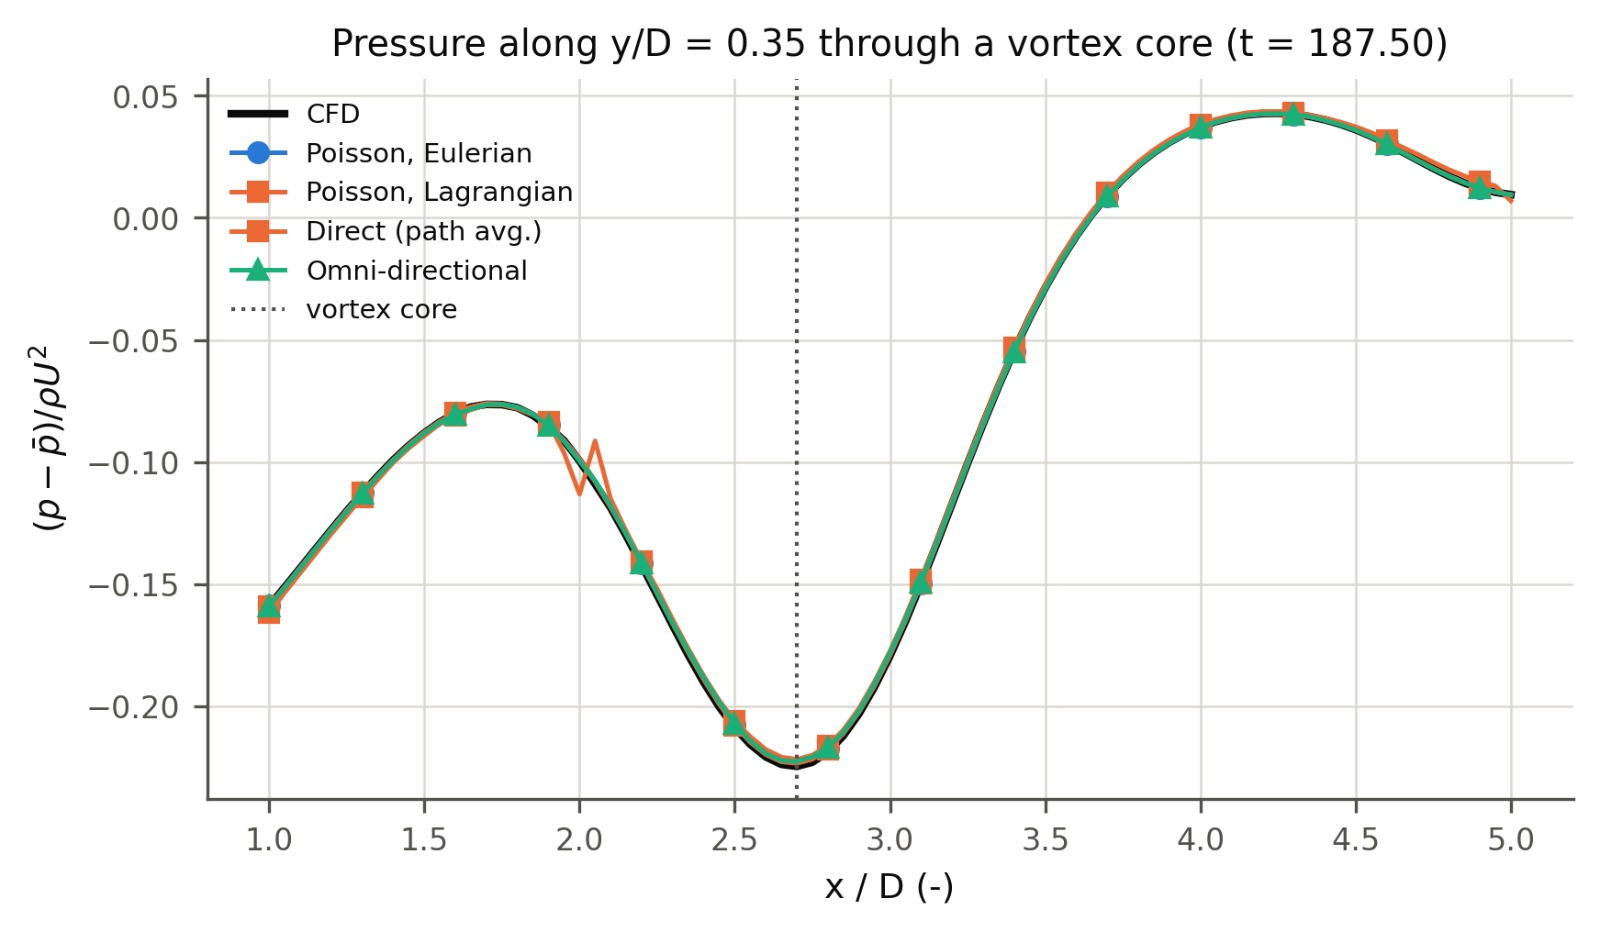
\includegraphics[width=0.75\linewidth]{img/c_line.png}
\caption{Pressure along $y/D=0.35$, through a shed vortex core: CFD and four reconstructions.}\end{figure}

\begin{enumerate}
\item \textbf{The wake pressure is recovered}: without noise the Poisson error is $\eps_{L2}=0.5$--0.75\,\% over a shedding period. All methods reproduce the vortex-core suction ($-0.22\rho U^2$ at $x/D\approx2.7$) within about 1\,\%.
\item \textbf{The error lies on the CFD mesh's block boundaries}: the vertical line $x/D=2$ and the diagonals towards $(2,\pm2)$ are exactly the edges of the O-grid around the cylinder, which extends to the square $[-2,2]^2$. The sampled velocity (interpolated from cell values) has small slope discontinuities across these block edges, where cell size and orientation change; differentiation turns these kinks into steps in $\G$. Direct integration, which carries every error along its path, shows a visible kink at $x/D=2$. This is a systematic error of the ``measured'' data, analogous to a calibration error in real PIV, and it is amplified by exactly the mechanism of Chapter~4.
\item \textbf{The largest error is near the inflow edge of the window} ($x/D\approx1$--1.7, $y<0$), where a new vortex is forming close to the cylinder and gradients are steepest.
\end{enumerate}

\subsection{Time step, scheme and noise on the wake}
\begin{figure}[H]\centering
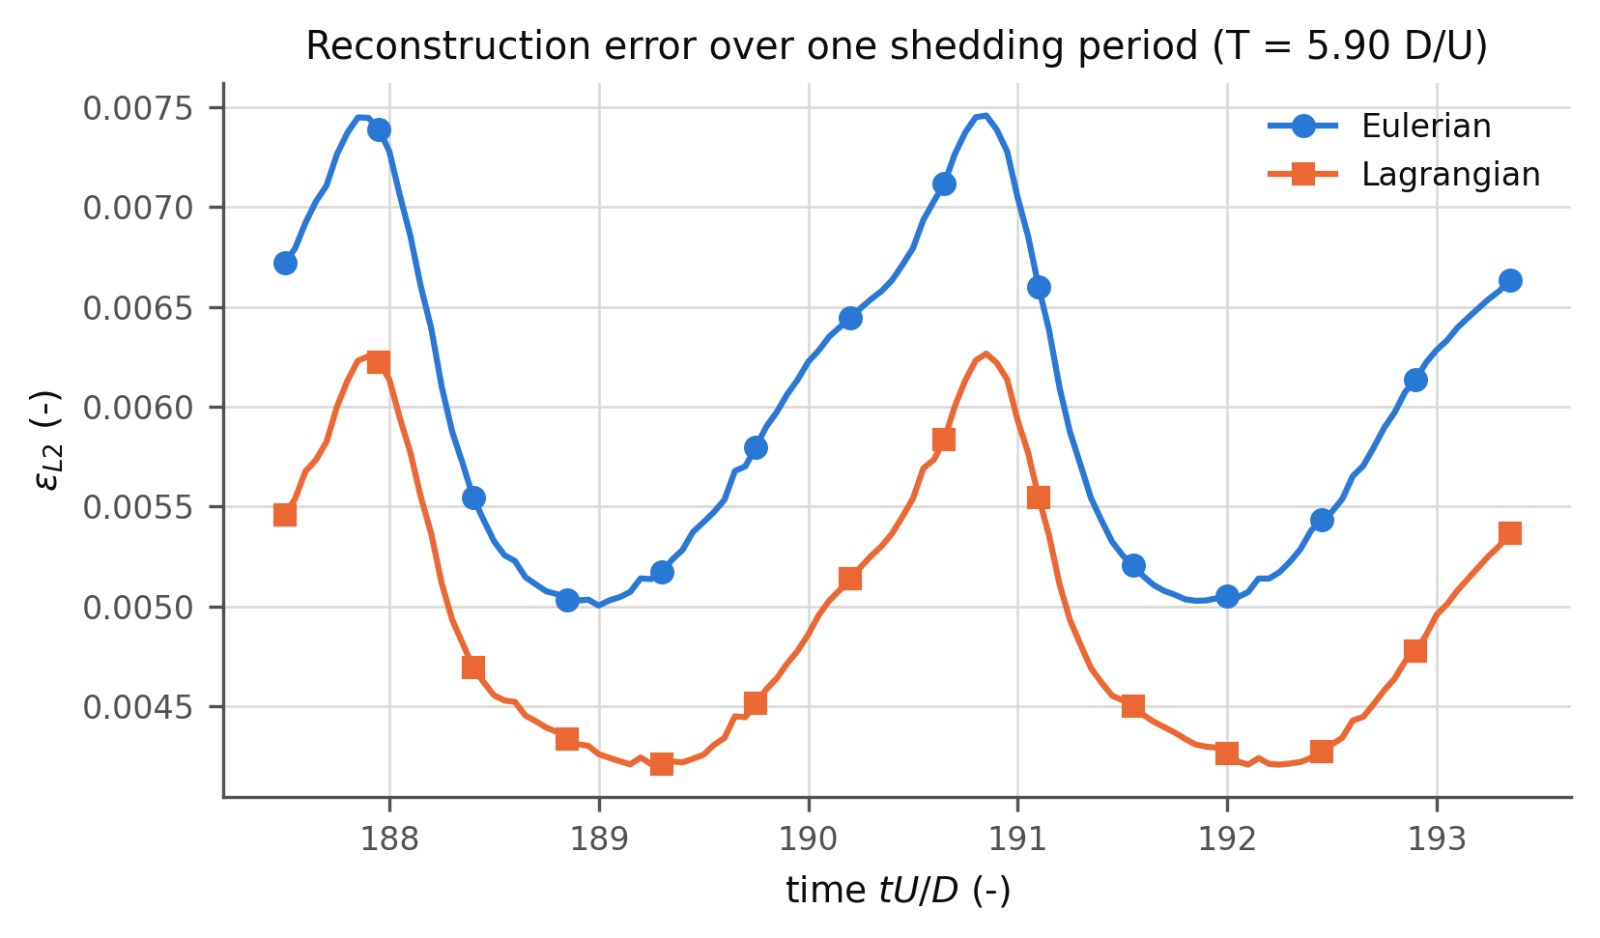
\includegraphics[width=0.62\linewidth]{img/c_period.png}\hfill
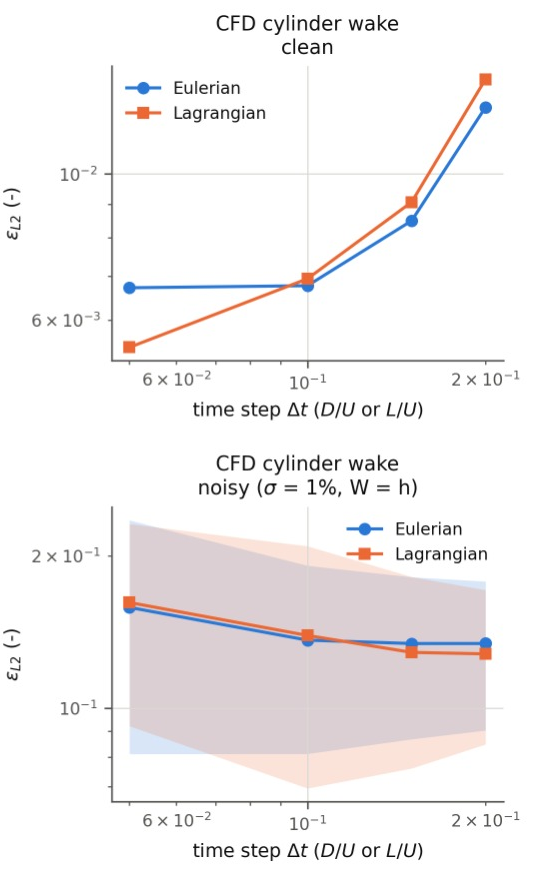
\includegraphics[width=0.3\linewidth]{img/c_dt_cfd.png}
\caption{Left: reconstruction error over one shedding period ($T=5.90$, clean, $\Delta t=0.05$). Right: error vs time step on the wake, clean (top) and with $\sigma=1\,\%$ noise (bottom).}\end{figure}

\begin{enumerate}
\item \textbf{The error pulses twice per shedding period} ($T=5.90$, so $St=1/T=0.1695$, consistent with the FFT). Each peak occurs as a new vortex forms on one side of the cylinder, near the inflow edge of the window.
\item \textbf{At $\Delta t=0.05$ the Lagrangian scheme is 15--18\,\% better} throughout the period ($\eps\approx0.0042$--0.0063 vs 0.0050--0.0075), as predicted for structures carried through the window.
\item \textbf{At $\Delta t\ge0.1$ the Eulerian scheme is slightly better} (e.g.\ $8.4\times10^{-3}$ vs $9.1\times10^{-3}$ at $\Delta t=0.15$), unlike the convected Taylor--Green vortex. The theory of Section~3.2 assumes a pattern simply carried along ($w\ll c$). In the near wake ($x/D=1$--5) the vortices are still forming: they move slower than $U_\infty$ and rotate quickly ($w$ comparable to $c$), so particle paths curve strongly and the straight-line tracking error grows quickly with $\Delta t$. More tracked points also leave the $4D\times4D$ window at larger $\Delta t$ and fall back to the Eulerian estimate. Both are plausible contributors; separating them would need the fallback fraction and a longer window.
\item \textbf{With 1\,\% noise} the error is $\eps\approx0.13$--0.15 for both schemes and almost flat in $\Delta t$: noise amplification dominates truncation. It is larger than on Taylor--Green (0.08) because the wake's pressure variations are only about $\pm0.2\rho U^2$, so the same velocity noise is larger relative to the signal.
\end{enumerate}

\begin{keyidea}[What the CFD case adds]
The analytic tests isolate each error source; the wake combines them on a realistic unsteady flow. The reconstruction recovers the wake pressure to better than 1\,\% from clean data, the Lagrangian advantage holds only at small $\Delta t$ in the vortex-formation region, and systematic kinks in the data (here from the CFD mesh) are amplified just like random noise.
\end{keyidea}

% ------------------------------------------------------------------
\chapter{Comparison with published studies}
The project's controlled synthetic experiments can be checked against the conclusions of the PIV-pressure literature.

\begin{table}[H]\centering\small
\begin{tabularx}{\linewidth}{@{}>{\raggedright\arraybackslash}X>{\raggedright\arraybackslash}Xl@{}}\toprule
This project & Published finding & Match\\\midrule
Exact $p$ on 2 edges: $\eps$ 0.044 vs 0.082 all-Neumann ($\approx2\times$) & Pan et al.\ (2016): Dirichlet boundaries give less error than Neumann (about 2$\times$ for large domains with boundary error); avoid pure Neumann where possible & Agrees\\
Bernoulli edges: $\eps$ 0.30--0.81 in rotational flow & Pan et al.\ (2016): Bernoulli-based Dirichlet data are valid only in irrotational regions & Agrees\\
Errors from 0.002\,\% (clean, fine) to $>100$\,\% (direct, $\sigma\ge2\,\%$); depend on method, spacing, filtering & Charonko et al.\ (2010), as summarised by Pan et al.: errors from $<1\,\%$ to $>100\,\%$, sensitive to all these factors, no single best method & Agrees\\
Lagrangian 3$\times$ better at large $\Delta t$ in convected flow; noise $\propto1/\Delta t$ & Violato et al.\ (2011): the Eulerian approach is limited to short $\Delta t$; short $\Delta t$ amplifies precision error, long $\Delta t$ adds truncation error & Agrees\\
Omni and Poisson recover the main features; direct integration very noise-sensitive & van Gent et al.\ (2017): all methods tested recover the main features; noise lowers accuracy but no method was critically sensitive at their noise levels & Partly\\
Cylinder wake (fine mesh): $St=0.1695$, $\bar C_D=1.388$, $C_L$ amplitude 0.345 & 2-D simulations at Re = 100 (e.g.\ Park et al.\ 1998): $St\approx0.164$--0.165, $\bar C_D\approx1.33$; experiments $St\approx0.164$ (Williamson 1996) & Agrees\\\bottomrule
\end{tabularx}\end{table}

\textbf{Why ``partly'' for van Gent et al.} Their comparison used tomographic PIV and Lagrangian particle tracking data with more advanced methods (least-squares pseudo-tracking, vortex-in-cell, FlowFit); simple single-path direct integration was not among them. Our direct-integration result does not contradict them, it covers a method they did not test.

\textbf{Why the wake values are 3--4\,\% high.} The $\pm10D$ symmetry sides block 5\,\% of the channel. The flow accelerates past the cylinder, which raises the drag and the shedding frequency; a few per cent is a plausible size for 5\,\% blockage, though we did not run a wider domain to confirm it. The literature values are for (nearly) unbounded domains and are quoted approximately; confirm them in the papers before quoting exact numbers.

\textbf{What the literature adds that we did not test.} Pan et al.\ show that the error also depends on the domain size and shape (for Dirichlet domains of fixed area, a square is the worst case). Our windows are all square, so this is a natural next study.

% ------------------------------------------------------------------
\chapter{Conclusions}

\section{Key findings}
\begin{enumerate}
\item \textbf{The code is verified.} All three algorithms are second-order accurate on exact Navier--Stokes solutions (slopes 1.8--2.1), including the boundaries.
\item \textbf{Noise, not discretisation, limits PIV pressure.} The error grows linearly with the velocity noise, and there is an optimum vector spacing ($h\approx0.03$ here) below which noise amplification by the derivatives dominates.
\item \textbf{The integration method matters.} Poisson and omni-directional integration are 5--7$\times$ more robust than direct integration because they average errors over many paths; Poisson is about 27$\times$ faster than omni.
\item \textbf{Boundary data matter.} Known pressure on two opposite edges halves the error; Bernoulli edges are valid only in irrotational flow; with pure Neumann data, a zero-mean constraint beats pinning a node.
\item \textbf{The time step is a trade-off.} The Lagrangian material derivative tolerates larger $\Delta t$ in convected flow; with noisy data a larger $\Delta t$ helps both schemes.
\item \textbf{Smoothing trades noise for bias.} Denoising cuts the noisy error about 3$\times$ but hurts clean data.
\item \textbf{The CFD wake.} The OpenFOAM solution is grid-independent (St = 0.1695, GCI 0.13\,\%) and periodic from $t=76$. From its velocity the pressure is reconstructed to 0.5--0.75\,\%; the remaining error sits on the CFD mesh's block edges, where kinks in the data are amplified like noise. The Lagrangian advantage holds only at small $\Delta t$ in the near wake.
\item \textbf{Solvers.} SOR (at the Neumann-corrected $\omega_{opt}$) and CG need 80--140$\times$ fewer iterations than Jacobi; classic Jacobi stalls on the all-Neumann problem; a small change per iteration is not proof of convergence.
\end{enumerate}

\section{Objectives}
All four objectives are met: the algorithms are implemented, verified on exact flows, studied parametrically, and compared with a CFD simulation and with published studies.

\begin{keyidea}[Main takeaway]
PIV pressure is limited by how velocity noise is amplified by differentiation. The choice of method, boundary data, vector spacing and time separation decides whether that noise is averaged out or accumulated.
\end{keyidea}

\section{Recommended practice}
Use a Poisson solver; impose Dirichlet values only where pressure is genuinely known (taps, free stream); use the Lagrangian material derivative with the largest $\Delta t$ that keeps truncation error small; choose the vector spacing near the noise--truncation optimum rather than the finest possible; apply light denoising above $\sigma\approx0.5\,\%$.

\section{Limitations and future work}
\begin{itemize}
\item \textbf{Noise model:} $\sigma$ is independent of the window size and uncorrelated between neighbouring vectors. Real PIV has less random error for larger windows and spatially correlated errors from overlapping windows.
\item \textbf{Two-dimensional data:} planar PIV of 3-D turbulence misses $-\rho w\,\partial\uu/\partial z+\mu\,\partial^2\uu/\partial z^2$, an $O(1)$ error that refinement cannot remove. The project includes a loader and out-of-plane term calculator for turbulence-database slices (JHTDB) but no data were analysed.
\item \textbf{Omni-directional method:} a rotating-ray variant of Liu \& Katz (2006), not a line-by-line copy.
\item \textbf{Domain shape:} only square windows were tested.
\item \textbf{CFD window:} the $4D\times4D$ window sits in the vortex-formation region and crosses mesh block edges; a window further downstream on a uniform-mesh region would separate the two effects.
\item \textbf{Next steps:} window-dependent noise; correlated noise; a downstream CFD window; 3-D time-resolved data.
\end{itemize}

% ================================================================== APPENDICES
\appendix

\chapter{Viva preparation: questions and short answers}
The questions below collect the ones already given in the chapters plus those an examiner is likely to ask about the whole project.

\section*{Big picture}
\begin{description}[style=nextline,leftmargin=0pt]
\item[Why is pressure from PIV an ill-posed / sensitive problem?] The data must be differentiated before being integrated, and differentiation amplifies noise as $1/h$, $1/h^2$ and $1/\Delta t$.
\item[What is the single most important result?] There is an optimum vector spacing: finer PIV grids can give worse pressure.
\item[Which method would you use in practice, and why?] Poisson: as robust as omni (both average errors), 27$\times$ faster, and well understood (least-squares projection).
\item[Why use synthetic data instead of a real experiment?] The true pressure must be known everywhere to measure the error. Exact solutions and CFD give it; one can also control each error source separately.
\end{description}

\section*{Physics}
\begin{description}[style=nextline,leftmargin=0pt]
\item[Derive the pressure gradient from Navier--Stokes.] Rearrange momentum: $\nabla p=-\rho D\uu/Dt+\mu\nabla^2\uu$.
\item[Why is Taylor--Green an exact solution?] $\nabla^2\uu=-2\uu$, so the unsteady and viscous terms cancel with $F=e^{-2\nu t}$, and the convective term is a gradient balanced by pressure.
\item[Why is the convected Taylor--Green exact?] Galilean invariance: $\uu'=\mathbf c+\uu(\mathbf x-\mathbf ct)$ has the same material derivative.
\item[What sets $\lambda$ in Kovasznay flow?] Substituting the ansatz gives $\lambda^2-Re\,\lambda-4\pi^2=0$; the negative root gives a decaying wake.
\item[When does the Lagrangian derivative beat the Eulerian one?] When structures are convected faster than their own velocity ($w<c$): errors scale as $w^3$ vs $c^3$.
\item[Why does Bernoulli fail here?] Both flows are rotational everywhere; Bernoulli holds across the field only in irrotational flow.
\end{description}

\section*{Numerics}
\begin{description}[style=nextline,leftmargin=0pt]
\item[Derive the one-sided first-derivative stencil.] Taylor-expand $f_1,f_2$; cancel $f_0$ and $f''$; get $(-3f_0+4f_1-f_2)/2h$.
\item[How are Neumann conditions imposed?] Ghost points eliminated with a central difference of the condition; corners use both conditions.
\item[Why is the all-Neumann system singular, and how do you fix it?] $A\mathbf1=0$; pin a node or add a zero-mean constraint (default).
\item[What is the compatibility residual?] $\iint\nabla\cdot\G-\oint\n\cdot\G$; non-zero when $\G$ is not an exact gradient.
\item[Why does Poisson filter noise?] It is the least-squares projection of $\G$ onto gradient fields; the curl is discarded.
\item[Why is direct integration path dependent?] Measured $\G$ has a curl; errors along a path add like a random walk.
\item[Why is the velocity-source Poisson form worse with noise?] Its source and its boundary data no longer come from one vector field, and it multiplies noisy derivatives.
\item[Why does an $O(h)$ boundary row still give $O(h^2)$ global error?] The error acts on an $O(h)$ strip; the scaled scheme is a second-order finite-volume scheme.
\end{description}

\section*{Solvers and convergence}
\begin{description}[style=nextline,leftmargin=0pt]
\item[Show Jacobi is pseudo-time marching.] $p^{k+1}=p^k+\Delta\tau(\nabla^2_hp^k-f)$, $\Delta\tau=\omega h^2/4$.
\item[Why does classic Jacobi stall?] The Neumann checkerboard mode has amplification $-1$.
\item[What is $\omega_{opt}$ for SOR here?] $2/(1+\sqrt{1-\rho_J^2})$ with $\rho_J=\cos^2(\pi h/2L)$ for Neumann walls: 1.932 at $64^2$.
\item[Why does SOR diverge for $\omega\ge2$?] Kahan: $\rho_{SOR}\ge|\omega-1|$.
\item[Is a small change per iteration enough to stop?] No; check the residual too. With slow convergence the true error is $\Delta/(1-\rho)$.
\item[Why normalise norms?] So the same physical imbalance gives the same number on any grid.
\end{description}

\section*{CFD}
\begin{description}[style=nextline,leftmargin=0pt]
\item[Why is a 2-D simulation valid at Re = 100?] The wake stays two-dimensional below Re $\approx$ 190.
\item[Why an O-grid?] Body-fitted, near-orthogonal cells, clustered at the wall for the boundary layer.
\item[Why the inlet kick?] A symmetric set-up delays shedding; the kick breaks symmetry and is removed at $t=6$.
\item[How is St computed?] FFT of $C_L(t)$ after uniform resampling and a Hann window; $St=fD/U$.
\item[Why might St and $C_D$ be higher than literature?] 5\,\% blockage from the $\pm10D$ symmetry sides.
\item[What does GCI = 0.5\,\% mean?] The fine-mesh value lies within about 0.5\,\% of the grid-converged value (safety factor 1.25).
\item[Why don't residuals fall to zero?] The flow is periodic; each step starts from a changed flow. Use a periodicity check instead.
\item[How does PISO relate to this project?] It solves a pressure Poisson equation from velocity every time step: the same mathematical step as the reconstruction.
\end{description}

% ------------------------------------------------------------------
\chapter{File map and how to run}

\section{Files}
\begin{table}[H]\centering\small
\begin{tabularx}{\linewidth}{@{}l>{\raggedright\arraybackslash}X@{}}\toprule
File & Role\\\midrule
\code{fields/field.py} & \code{FlowField}, the common data interface\\
\code{fields/analytic.py} & Taylor--Green (incl.\ convected) and Kovasznay solutions\\
\code{fields/cfd\_loader.py}, \code{jhtdb\_loader.py} & CFD window and turbulence-database loaders\\
\code{piv/degrade.py}, \code{denoise.py} & synthetic PIV model; Gaussian and Savitzky--Golay filters\\
\code{core/derivatives.py} & finite-difference stencils (order 1 or 2)\\
\code{core/material\_derivative.py} & Eulerian/Lagrangian $D\uu/Dt$ and $\G$\\
\code{core/poisson.py} & matrix assembly, ghost points, compatibility, direct/CG solve\\
\code{core/iterative.py} & Jacobi, Gauss--Seidel, SOR, CG with residual histories\\
\code{core/direct\_integration.py}, \code{omni\_integration.py} & the other two integration methods\\
\code{core/pipeline.py} & \code{reconstruct()}, the single entry point\\
\code{analysis/metrics.py}, \code{norms.py} & error metrics and residual norms\\
\code{analysis/plots.py}, \code{summary.py} & shared plot style; \code{SUMMARY.md} generator\\
\code{studies/run\_*.py} & one script per parameter sweep\\
\code{cfd/generate\_cases.py} & writes the OpenFOAM cases and \code{mesh\_info.json}\\
\code{cfd/cases/*/Allrun} & mesh and run one case (serial or parallel)\\
\code{cfd/export\_window.py} & window samples $\to$ \code{cylinder\_re100\_window.npz}\\
\code{cfd/grid\_independence.py} & St, $C_D$, $C_L$, Richardson/GCI\\
\code{cfd/parse\_log.py}, \code{change\_norm.py} & solver residuals; periodicity check\\
\code{tests/} & 87 unit tests\\
\code{run\_all.py} & runs every study and the summary\\\bottomrule
\end{tabularx}\end{table}

\section{Commands}
Analytic studies (any OS, from \code{piv\_pressure/}):
\begin{lstlisting}
python -m pip install -r requirements.txt
python -m pytest -q            # 87 passed
python run_all.py --quick      # ~40 s check
python run_all.py              # full run, ~8 min
\end{lstlisting}
\needspace{16\baselineskip}
CFD on native Windows with the OpenFOAM MinGW build (OpenFOAM terminal for the runs, PowerShell for Python):
\begin{lstlisting}
python cfd/generate_cases.py                              # PowerShell
sed -i 's/\r$//' cfd/cases/*/Allrun                       # OpenFOAM terminal
sed -i 's/mpirun -np/mpiexec -n/' cfd/cases/*/Allrun      # MS-MPI only has mpiexec
sh cfd/cases/coarse/Allrun 4
sh cfd/cases/medium/Allrun 4
sh cfd/cases/fine/Allrun 4
python cfd/grid_independence.py                           # PowerShell, after the runs
python cfd/export_window.py
python cfd/parse_log.py
python cfd/change_norm.py
python run_all.py
\end{lstlisting}

% ------------------------------------------------------------------
\chapter{Notation}
\begin{table}[H]\centering\small
\begin{tabular}{@{}ll@{}}\toprule
Symbol & Meaning\\\midrule
$\uu=(u,v)$ & velocity\\
$p$, $p_{ref}$ & reconstructed and true pressure (kinematic in CFD, $\rho=1$)\\
$\rho,\ \mu,\ \nu=\mu/\rho$ & density, dynamic and kinematic viscosity\\
$\G$ & pressure gradient estimated from velocity, $-\rho D\uu/Dt+\mu\nabla^2\uu$\\
$h$ ($\Delta x,\Delta y$) & PIV vector spacing\\
$W$ & interrogation-window width\\
$\sigma$ & velocity noise level, fraction of $U$\\
$\Delta t$ & time between PIV snapshots\\
$\eps_{L2},\ \eps_{max}$ & relative $L_2$ error; max error over $\tfrac12\rho U^2$\\
$R$ & compatibility residual\\
$A,\ b,\ w$ & Poisson matrix, right-hand side, trapezoidal weights\\
$\omega$ & relaxation factor (Jacobi, SOR)\\
$\rho_J,\ \rho_{SOR}$ & spectral radii of the iteration matrices\\
$St,\ C_D,\ C_L$ & Strouhal number, drag and lift coefficients\\
$p$ (Richardson), GCI & observed order; grid convergence index\\\bottomrule
\end{tabular}\end{table}

% ------------------------------------------------------------------
\chapter*{References}
\addcontentsline{toc}{chapter}{References}
\begin{enumerate}[label={[\arabic*]},leftmargin=*]
\item B.\,W.\ van Oudheusden, PIV-based pressure measurement, \emph{Meas.\ Sci.\ Technol.}\ 24 (2013) 032001.
\item J.\,J.\ Charonko, C.\,V.\ King, B.\,L.\ Smith, P.\,P.\ Vlachos, Assessment of pressure field calculations from particle image velocimetry measurements, \emph{Meas.\ Sci.\ Technol.}\ 21 (2010) 105401.
\item Z.\ Pan, J.\ Whitehead, S.\ Thomson, T.\ Truscott, Error propagation dynamics of PIV-based pressure field calculations: how well does the pressure Poisson solver perform inherently?, \emph{Meas.\ Sci.\ Technol.}\ 27 (2016) 084012. \url{https://arxiv.org/abs/1602.00037}
\item P.\,L.\ van Gent et al., Comparative assessment of pressure field reconstructions from particle image velocimetry measurements and Lagrangian particle tracking, \emph{Exp.\ Fluids} 58 (2017).
\item X.\ Liu, J.\ Katz, Instantaneous pressure and material acceleration measurements using a four-exposure PIV system, \emph{Exp.\ Fluids} 41 (2006) 227--240.
\item D.\ Violato, P.\ Moore, F.\ Scarano, Lagrangian and Eulerian pressure field evaluation of rod--airfoil flow from time-resolved tomographic PIV, \emph{Exp.\ Fluids} 50 (2011) 1057--1070.
\item R.\ de Kat, B.\,W.\ van Oudheusden, Instantaneous planar pressure determination from PIV in turbulent flow, \emph{Exp.\ Fluids} 52 (2012).
\item J.\ Park, K.\ Kwon, H.\ Choi, Numerical solutions of flow past a circular cylinder at Reynolds numbers up to 160, \emph{KSME Int.\ J.}\ 12 (1998) 1200--1205.
\item C.\,H.\,K.\ Williamson, Vortex dynamics in the cylinder wake, \emph{Annu.\ Rev.\ Fluid Mech.}\ 28 (1996) 477--539.
\item L.\,I.\,G.\ Kovasznay, Laminar flow behind a two-dimensional grid, \emph{Proc.\ Camb.\ Philos.\ Soc.}\ 44 (1948) 58--62.
\item I.\,B.\ Celik et al., Procedure for estimation and reporting of uncertainty due to discretization in CFD applications, \emph{J.\ Fluids Eng.}\ 130 (2008) 078001.
\item D.\,M.\ Young, \emph{Iterative Solution of Large Linear Systems}, Academic Press, 1971.
\end{enumerate}
\textit{Notes.} The findings attributed to [3], [4] and [6] were checked against the papers' abstracts or text; [2] as summarised in [3]. Literature values for the cylinder wake ([8]) are approximate and should be confirmed from the paper before quoting.


\end{document}
